%%%%%%%%%%%%%%%%%%%%%%%%%%%%%%%%%%%%%%%%%%%%%%%%%%%%%%%%%%%%%%%%%%%%%%%%%%%%%%%%%%%%%%%%%%%%%%%%%%%%%%%%%%%%%%%%%%%%%%%%%%%%%%%%%%%%%%%%%%%%%%%%%%%%%%%%%%%%%%%%%%%%%%%%%%%%%%%%%%%%%%%%%%%%%%%%%%%%%%%%%%%%%%%%%%%%%%%%%%%%%%%%%%%%%%%%%%%
%%%%%%%%%%%%%%%%%%%%%%%%%%%%%%%%%%%%%%%%%%%%%%%%%%%%%%%%%%%%%%%%%%%%%%%%%%%%%%%%%%%%%%%%%%%%%%%%%%%%%%%%%%%%%%%%%%%%%%%%%%%%%%%%%%%%%%%%%%%%%%%%%%%%%%%%%%%%%%%%%%%%%%%%%%%%%%%%%%%%%%%%%%%%%%%%%%%%%%%%%%%%%%%%%%%%%%%%%%%%%%%%%%%%%%%%%%%
%%%%%%%%%%%%%%%%%%%%%%%%%%%%%%%%%%%%%%%%%%%%%%%%%%%%%%%%%%%%%%%%%%%%%%%%%%%%%%%%%%%%%%%%%%%%%%%%%%%%%%%%%%%%%%%%%%%%%%%%%%%%%%%%%%%%%%%%%%%%%%%%%%%%%%%%%%%%%%%%%%%%%%%%%%%%%%%%%%%%%%%%%%%%%%%%%%%%%%%%%%%%%%%%%%%%%%%%%%%%%%%%%%%%%%%%%%%
\chapter{Introduction}
\label{res:ch:Introduction}

The determination and quantification of the quality of the jet transverse-momentum measurement is of crucial interest for many analyses with jet final states, \eg the measurement of the dijet cross section~\cite{bib:CMS:QCD_measurements} or \ttbar production cross sections~\cite{bib:CMS:TopCrossSection_8TeV}. 
Also searches for physics beyond the standard model with missing transverse momentum, \PTm, in the final state need a good knowledge of \PTm originating from wrongly measured jets~\cite{bib:CMS:RA2_8TeV,bib:CMS:MT2_8TeV,bib:CMS:AlphaT_8TeV}.
For analyses relying on information from simulation it is very important to correct the simulated resolution to the resolution actually present in data.
Therefore, scale factors will be presented to adjust the resolution in simulation to the resolution of the real detector.  
  
In the following sections, a data-based method to measure the jet \pt resolution in \GAMJET events will be presented. 
A similar method was already accomplished in earlier analyses~\cite{bib:CMS:JERCPaper_2011,bib:CMS-AN-2010-076,bib:CMS-AN-2010-141,bib:CMS-AN-2011-004} of 7\tev data.  
It is further developed here and applied to 8\tev data.

The method is based on the transverse-momentum balance in the \GAMJET system. 
It takes advantage of the high resolution of the electromagnetic calorimeter and hence the excellent measurement of the photon energy and momentum.
Without initial and final state radiation, the photon and the jet are balanced in the transverse plane. 
Thus, measuring the photon \pt with high accuracy leads to an estimate of the true jet transverse momentum offering a possibility to quantify the resolution of jet \pt measurements.


%%%%%%%%%%%%%%%%%%%%%%%%%%%%%%%%%%%%%%%%%%%%%%%%%%%%%%%%%%%%%%%%%%%%%%%%%%%%%%%%%%%%%%%%%%%%%%%%%%%%%%%%%%%%%%%%%%%%%%%%%%%%%%%%%%%%%%%%%%%%%%%%%%%%%%%%%%%%%%%%%%%%%%%%%%%%%%%%%%%%%%%%%%%%%%%%%%%%%%%%%%%%%%%%%%%%%%%%%%%%%%%%%%%%%%%%%%%
%%%%%%%%%%%%%%%%%%%%%%%%%%%%%%%%%%%%%%%%%%%%%%%%%%%%%%%%%%%%%%%%%%%%%%%%%%%%%%%%%%%%%%%%%%%%%%%%%%%%%%%%%%%%%%%%%%%%%%%%%%%%%%%%%%%%%%%%%%%%%%%%%%%%%%%%%%%%%%%%%%%%%%%%%%%%%%%%%%%%%%%%%%%%%%%%%%%%%%%%%%%%%%%%%%%%%%%%%%%%%%%%%%%%%%%%%%%
%%%%%%%%%%%%%%%%%%%%%%%%%%%%%%%%%%%%%%%%%%%%%%%%%%%%%%%%%%%%%%%%%%%%%%%%%%%%%%%%%%%%%%%%%%%%%%%%%%%%%%%%%%%%%%%%%%%%%%%%%%%%%%%%%%%%%%%%%%%%%%%%%%%%%%%%%%%%%%%%%%%%%%%%%%%%%%%%%%%%%%%%%%%%%%%%%%%%%%%%%%%%%%%%%%%%%%%%%%%%%%%%%%%%%%%%%%%
\FloatBarrier
\chapter{General approach of the resolution measurement using photon+jet events}
\label{res:ch:GeneralApproach}

The jet transverse-momentum resolution is defined as the standard deviation of the jet transverse-momentum response distribution with the response defined as the ratio of the reconstructed to the generator-level jet transverse momentum 
\begin{equation}\label{res:eq:responseFormula}
\mathcal{R} =  \frac{\ptrecojet}{\ptgenjet}.
\end{equation}
For each reconstructed jet, the underlying generator-level jet is hereby found by matching the closest generator-level jet to the reconstructed jet with $\Delta R = \sqrt{(\Delta \phi)^2 + (\Delta \eta)^2}$ with a maximal $\Delta R_{\text{max}}=0.25$.
Furthermore, the transverse momentum of the generator-level jet is defined as the sum of all particles' transverse momenta that are clustered into the jet cone.
It can therefore differ to the momentum of the original final state quark or gluon by out-of-cone showering effects.
Out-of-cone showering refers to particles from the hadronisation process that are not clustered into the jet cone.
Throughout the following sections, the jet transverse-momentum resolution will be abbreviated JER\footnote{This abbreviation is a historical relic from experiments where the momentum of jets were only measured in the calorimeters and therefore JER refered to jet energy resolution.}.
The mean of the response distribution will be referred to as jet energy scale.

Figure~\ref{res:fig:TypicalResponse} shows a response distribution for jets in the barrel region.
\begin{figure}[b]
  \centering
      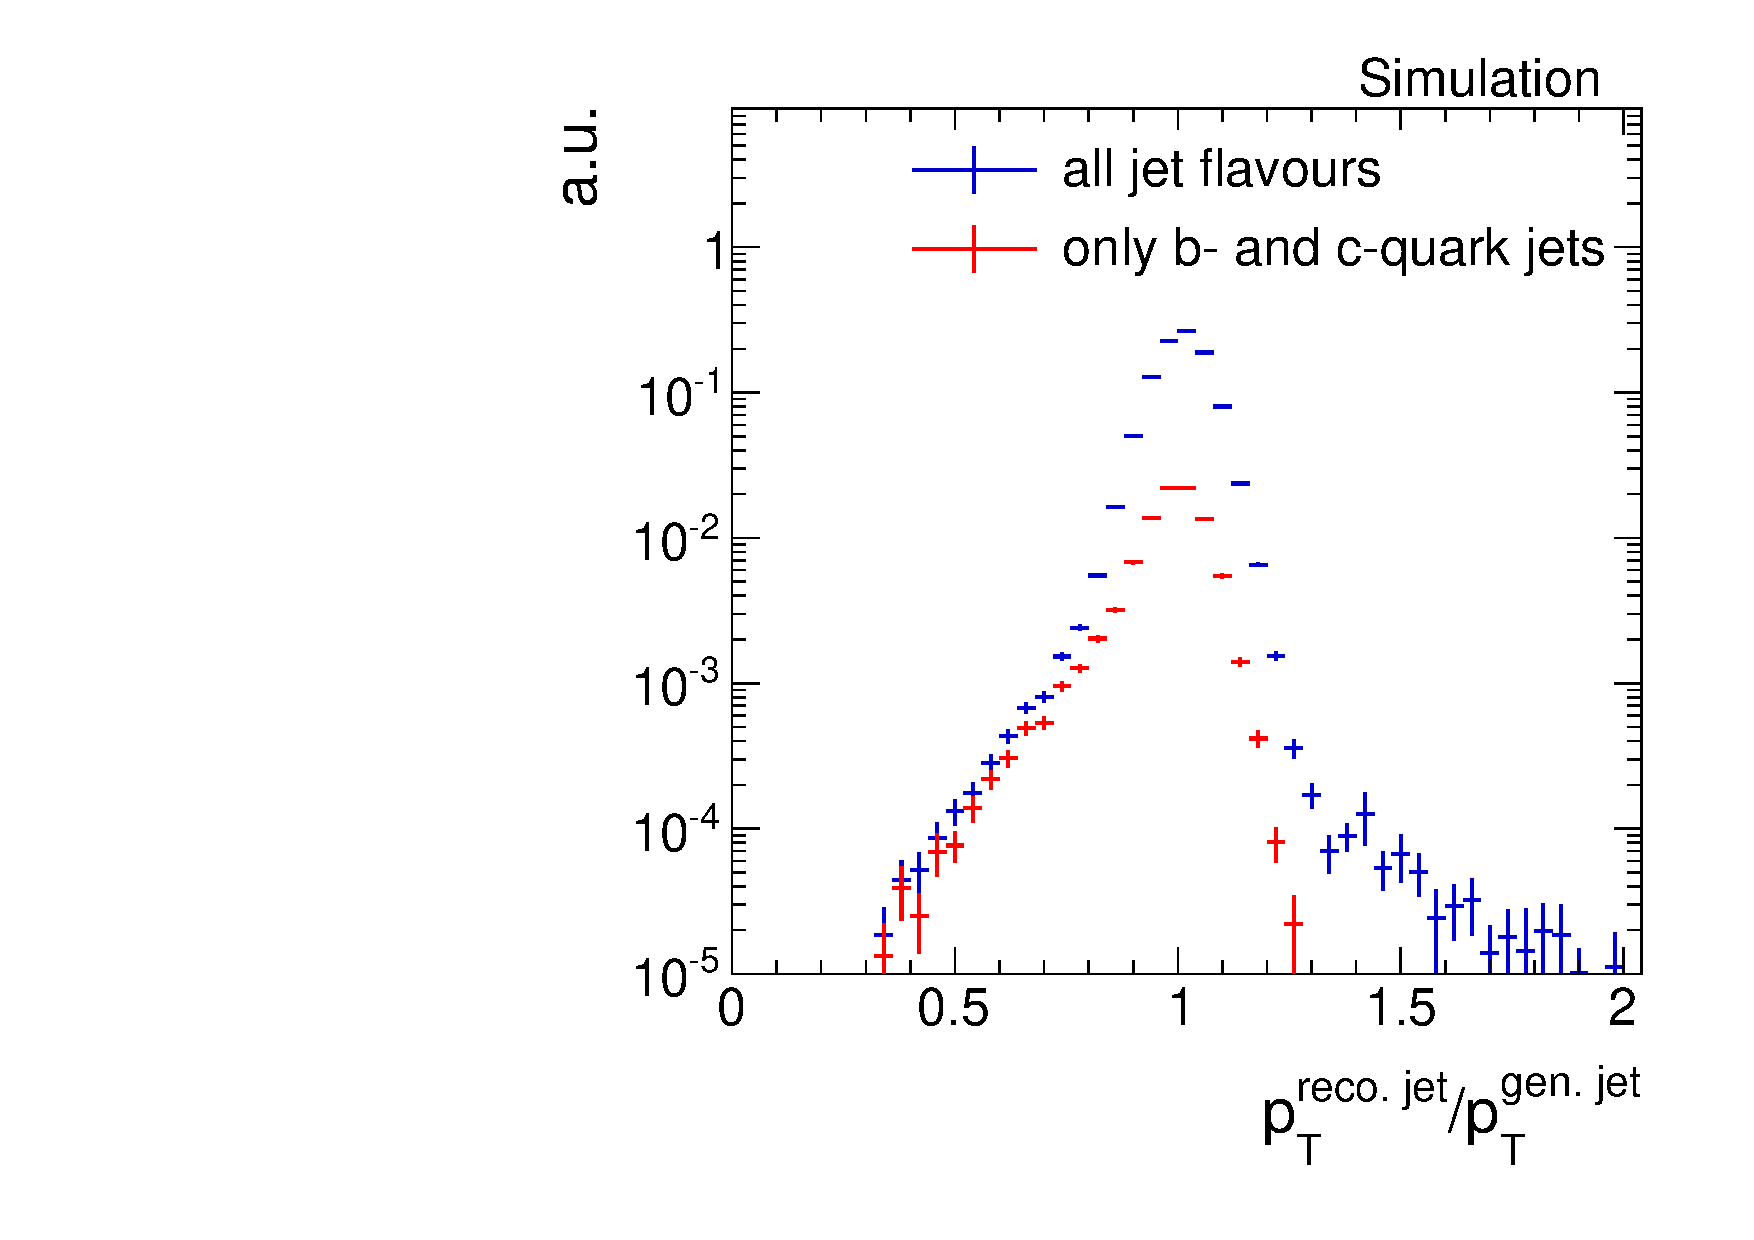
\includegraphics[width=0.49\textwidth]{figures/resolution/generalApproach/intrinsicExampleContributionofBCQuarks.pdf}
  \caption{Number of events over $\frac{\pt^{\text{reco. jet}}}{\pt^{\text{gen. jet}}}$ from a simulated \GAMJET sample. 
           The black dots show the contribution by c- and b-quark jets where the left tail originating from semi-leptonic decays of heavy quarks can be seen.}  
  \label{res:fig:TypicalResponse}
\end{figure}
The core of the response distribution shows the typical Gaussian behavior whereas the tails deviate from that functional form.
Physical reasons for the low response tail are inter alia semi-leptonic decays of heavy quarks where the neutrino cannot be detected and the reconstructed transverse momentum of the jet is too small.
This effect is visible in Fig.~\ref{res:fig:TypicalResponse} because the neutrinos are included into the generator-level jet.
Some instrumental effects, such as a non-linear response of the calorimeter, inhomogeneities of the detector material and electronic noise can contribute to both tails, 
others, like dead calorimeter channels only contribute to the left tail. 
The resolution is therefore determined using only the core of the distribution to avoid the coverage of non-Gaussian tails.
The resolution is thus defined as the standard deviation of the 99\% truncated response histogram devided by the mean of the histogram:

\begin{equation*}\label{res:eq:resolutionFormula}
\jer = \frac{\sigma_{99\%}}{\mu_{99\%}}.
\end{equation*}

The determination of the 99\% range of the histogram is done in several steps. 
First the mean of the core is found via a Gaussian fit to the histogram in a 2$\sigma$ range\footnote{The 2$\sigma$ range is defined as the range [$\mu - 2\sigma$,$\mu + 2\sigma$].}. 
This procedure is done in three iteration steps.
Then, a symmetric interval around this mean is determined with its integral equal to 99\% of the integral of the full histogram. 
The division by the mean aims to make the resolution independent of the absolute scale of the response histogram.
Since after the application of the jet energy corrections the scale is anyways very close to one, this is only a tiny effect.

%The division by the mean is done to make the resolution measurement more insensitive to a variation of the jet energy scale (= mean of the response distribution)
%which has also an effect on the measured width of the distribution. 
%because response distributions with a scale smaller than one are typically narrower while distributions with scales larger than one are broader.

The evaluation of the response distribution as reconstructed over generator-level jet transverse momentum (Eq.~\eqref{res:eq:responseFormula})
is only possible for simulated events where generator-level information is accessible. 
A determination of the resolution in data, however, has to rely on a different approach.\\

The main idea of a resolution measurement using \GAMJET events is based on the transverse-momentum balance of the \GAMJET system and the excellent electromagnetic calorimeter resolution
(which was estimated between 1.1 \% and 3.8\% in the barrel region for photons for $\sqrt{s}=8\tev$ data~\cite{bib:CMS:PhotonResolution_8TeV}).

In Fig~\ref{res:fig:FeynmanDiagrams}, all tree-level processes contributing to an event topology with one photon and one jet in the final state are depicted. 
\begin{figure}[b]
  \centering
      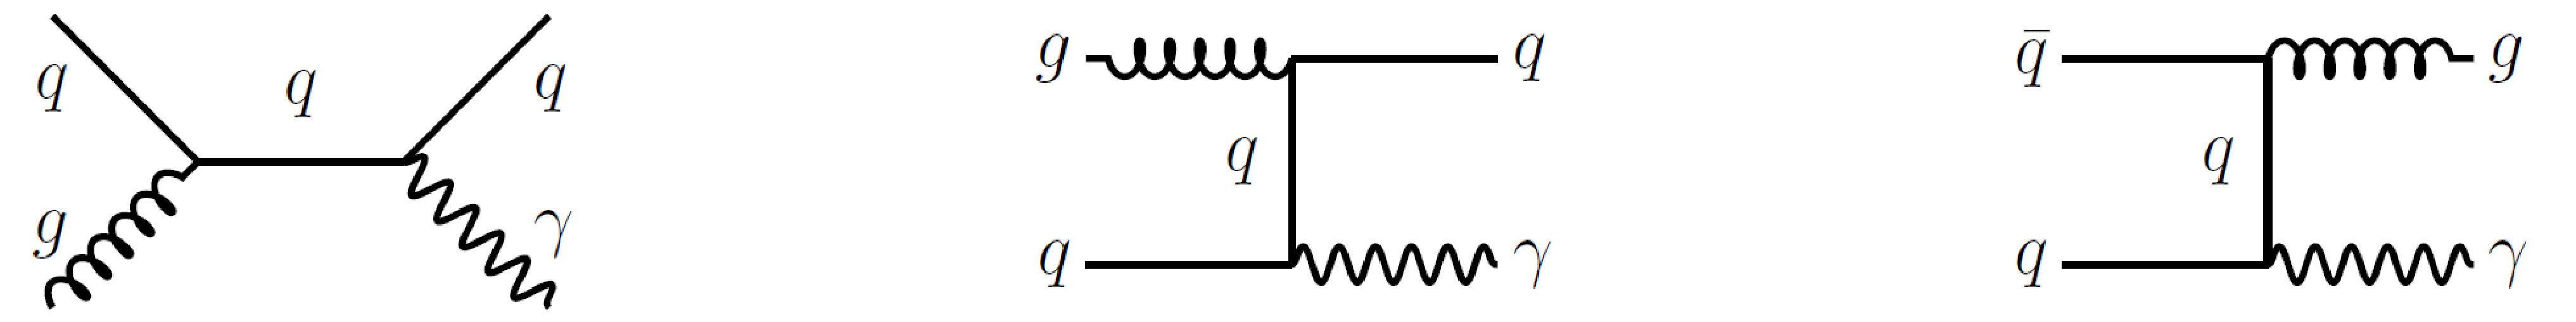
\includegraphics[width=0.99\textwidth]{figures/resolution/generalApproach/FeynmanDiagram.pdf}
  \caption{Tree-level Feynman diagrams of processes at the LHC in pp collisions with one photon and one jet in the final state.}  
  \label{res:fig:FeynmanDiagrams}
\end{figure}
Due to momentum conversation, the jet and the photon are back to back in the transverse plane, and therefore, $\ptvec^{\,\gamma} = -\ptvec^{\,\text{jet}}$. 
Because of the good resolution of the electromagnetic calorimeter, photon momenta can be very well measured 
and thus can serve as an excellent estimator for the true jet momentum.


Unfortunately, such clean events are very rare processes, and usually, the momentum balance is spoiled by initial and final state radiation, which lead to further jets in the event 
(see Fig.~\ref{res:fig:FeynmanDiagramsWithRadiation}). 
However, in order to select events that are balanced to a large extent, a lower bound 
on the angular distance in the transverse plane between the photon and the jet with the highest transverse momentum (leading jet) is required: $\Delta\Phi \left(\text{\nth{1} jet, } \gamma \right)>2.95\,\unit{rad}$. 

Additionally, the variable 
\begin{equation*}\label{res:eq:alphaDef}
\alpha \doteq \frac{\ptsecondrecojet}{\ptgamma}
\end{equation*} 
is defined as a measure of further jet activity in an event. 
It is, however, not sufficient to require only an upper bound on $\alpha$. 
Instead, the jet energy resolution is measured in bins of $\alpha$ (with max($\alpha$) = 0.2), 
and the extrapolated value to zero further jet energy ($\alpha=0$) is taken as the measured resolution of the jet energy in the absence of further jets.
\begin{figure}[t]
  \centering
      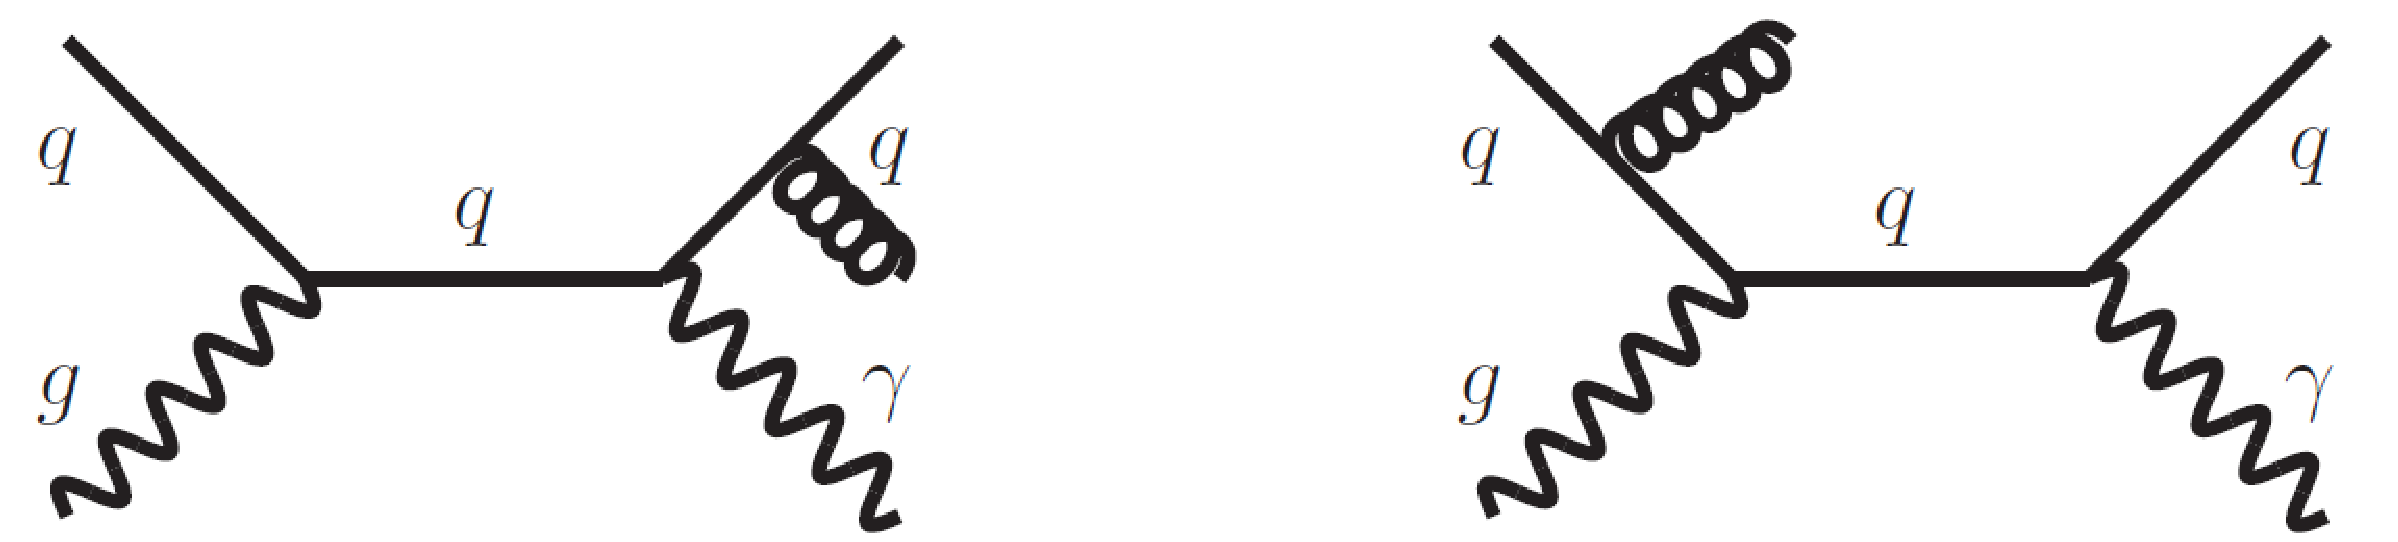
\includegraphics[width=0.60\textwidth]{figures/resolution/generalApproach/FeynmanDiagramsWithRadiation.pdf}
  \caption{Tree-level Feynman diagrams with initial and final state radiation.}  
  \label{res:fig:FeynmanDiagramsWithRadiation}
\end{figure}

Measuring the transverse momentum of the photon instead of taking the generator-level jet \pt leads to the fact that the measured resolution consists out of two parts
\begin{equation*}\label{res:eq:splitting}
\frac{\ptrecojet}{\ptgamma} = \underbrace{\frac{\ptrecojet}{\ptgenjet}}_{\text{intrinsic}} \cdot \underbrace{\frac{\ptgenjet}{\ptgamma}}_{\text{imbalance}}.
\end{equation*}
The intrinsic part is the resolution of interest which is independent of further jets in the event whereas the imbalance is strongly dependent on $\alpha$.

To extract the intrinsic resolution out of the measured one, the residual imbalance $q$ (the imbalance at $\alpha = 0$) is subtracted from the total resolution in the 
limit of vanishing additional jet activity. 
As that information is only available from simulation, the measured resolution in data is corrected by the residual imbalance taken from the simulated dataset.
%%%%%%%%%%%%%%%%%%%%%%%%%%%%%%%%%%%%%%%%%%%%%%%%%%%%%%%%%%%%%%%%%%%%%%%%%%%%%%%%%%%%%%%%%%%%%%%%%%%%%%%%%%%%%%%%%%%%%%%%%%%%%%%%%%%%%%%%%%%%%%%%%%%%%%%%%%%%%%%%%%%%%%%%%%%%%%%%%%%%%%%%%%%%%%%%%%%%%%%%%%%%%%%%%%%%%%%%%%%%%%%%%%%%%%%%%%%

%%%%%%%%%%%%%%%%%%%%%%%%%%%%%%%%%%%%%%%%%%%%%%%%%%%%%%%%%%%%%%%%%%%%%%%%%%%%%%%%%%%%%%%%%%%%%%%%%%%%%%%%%%%%%%%%%%%%%%%%%%%%%%%%%%%%%%%%%%%%%%%%%%%%%%%%%%%%%%%%%%%%%%%%%%%%%%%%%%%%%%%%%%%%%%%%%%%%%%%%%%%%%%%%%%%%%%%%%%%%%%%%%%%%%%%%%%%
%%%%%%%%%%%%%%%%%%%%%%%%%%%%%%%%%%%%%%%%%%%%%%%%%%%%%%%%%%%%%%%%%%%%%%%%%%%%%%%%%%%%%%%%%%%%%%%%%%%%%%%%%%%%%%%%%%%%%%%%%%%%%%%%%%%%%%%%%%%%%%%%%%%%%%%%%%%%%%%%%%%%%%%%%%%%%%%%%%%%%%%%%%%%%%%%%%%%%%%%%%%%%%%%%%%%%%%%%%%%%%%%%%%%%%%%%%%
\FloatBarrier
\chapter{Datasets and event selection}

The measurement of the jet energy resolution is carried out with \GAMJET data recorded during the year 2012 at the CMS experiment.
The datasets and triggers that are exploitet for this measurement are introduced in the following Section~\ref{res:sec:DatasetsAndTriggers}.
In order to select \GAMJET events that are well suited for the resolution measurement, an event selection is applied on top. % to ensure \GAMJET events that show already the disired back-to-back signatures.
This event selection is described in Section~\ref{res:sec:EventSelection}.

\section{Datasets and triggers}
\label{res:sec:DatasetsAndTriggers}
This analysis exploits several triggers which were active during the year 2012 at the CMS experiment.
Because of the high production cross section of \GAMJET events, especially for low photon \pt, almost all of these triggers were highly prescaled, \ie only a fraction of events were actually recorded when the triggers fired.
All triggers that are utilised in this measurement are listed in Table~\ref{res:tab:triggers} together with their recorded luminosity.
\renewcommand{\arraystretch}{1.5}
\begin{table}[!hbt]
\centering
\caption{Single-photon triggers together with the recorded luminosity taking the prescales of the triggers into consideration.}
\label{res:tab:triggers}
\makebox[0.99\textwidth]{
\begin{tabular}{lr}
\multicolumn{2}{c}{} \\
\toprule
Trigger                       & Luminosity [\fbinv]   \\
\midrule
HLT\_Photon20\_CaloIdVL\_IsoL & 0.0008\\
HLT\_Photon30\_CaloIdVL\_IsoL & 0.0029\\
HLT\_Photon50\_CaloIdVL\_IsoL & 0.0607\\
HLT\_Photon75\_CaloIdVL\_IsoL & 0.123\\
HLT\_Photon90\_CaloIdVL\_IsoL & 0.373\\
HLT\_Photon135\               & 13.77\\
HLT\_Photon150\               & 19.71\\
\bottomrule
\multicolumn{2}{c}{} \\
\end{tabular}}
\end{table}  
The triggers rely on level one on single-photon triggers, such as L1SingleEG12 and L1SingleEG30.
The L1 triggers require at least one photon that is above a certain \pt threshold, \eg 12\gev or 30\gev.
The high-level triggers require a photon with a certain \pt (as indicated in the name) and, in case of thresholds below 135\gev also additional quality and isolation criteria. 
All triggers with threshold below 150\gev were prescaled.

The events that are selected by the above mentioned triggers are contained in the datasets listed in Table~\ref{res:tab:datasets}.
\renewcommand{\arraystretch}{1.5}
\begin{table}[!hbt]
\centering
\caption{Single-photon data samples used for the resolution measurement with the contained integrated luminosity.}
\label{res:tab:datasets}
\makebox[0.99\textwidth]{
\begin{tabular}{l r}
\multicolumn{2}{c}{} \\
\toprule
Dataset                                          & Luminosity [\fbinv]   \\
\midrule
 /Photon/Run2012A-22Jan2013-v1/AOD               &  0.876   \\
 /SinglePhoton/Run2012B-22Jan2013-v1/AOD         &  4.412  \\
 /SinglePhoton/Run2012C-22Jan2013-v1/AOD         &  7.055  \\
 /SinglePhotonParked/Run2012D-22Jan2013-v1/AOD   &  7.354  \\ 
\bottomrule
\multicolumn{2}{c}{} \\
\end{tabular}}
\end{table}  

\section{Simulated samples}
\label{res:sec:SimulatedSamples}

FIXME: What about QCD multijet sample -  maybe mentione here.
In order to compare the measured resolution in data to the resolution in simulation, a single-photon sample simulated with \pythiaSix is used.
This sample was generated flat in the photon \pt to have a good statistical precision also for the high photon \pt region.
In order to recover a physical \pt spectrum, all simulated events are reweighted.
Figure~\ref{res:fig:PhotonPtSpectrum} shows the photon \pt spectrum in simulation before and after the reweighting. 

All simulated samples come with a pileup scenario which does not necessarily match the pileup scenario in data. 
To match the measured distribution of primary vertices, the events are weighted according to their number of primary vertices. 
Because almost all of the used triggers are differently prescaled, the distributions of primary vertices differ among the various events triggered by the corresponding trigger.
Thus the reweighing has to be done separately for the events falling in the photon \pt range of the several triggers (see Table~\ref{res:tab:PhotonPtBins}).
A comparison between the number of primary vertices can be found in Appendix~\ref{res:app:pileup} for all triggers.
\begin{figure}[h]
  \centering
      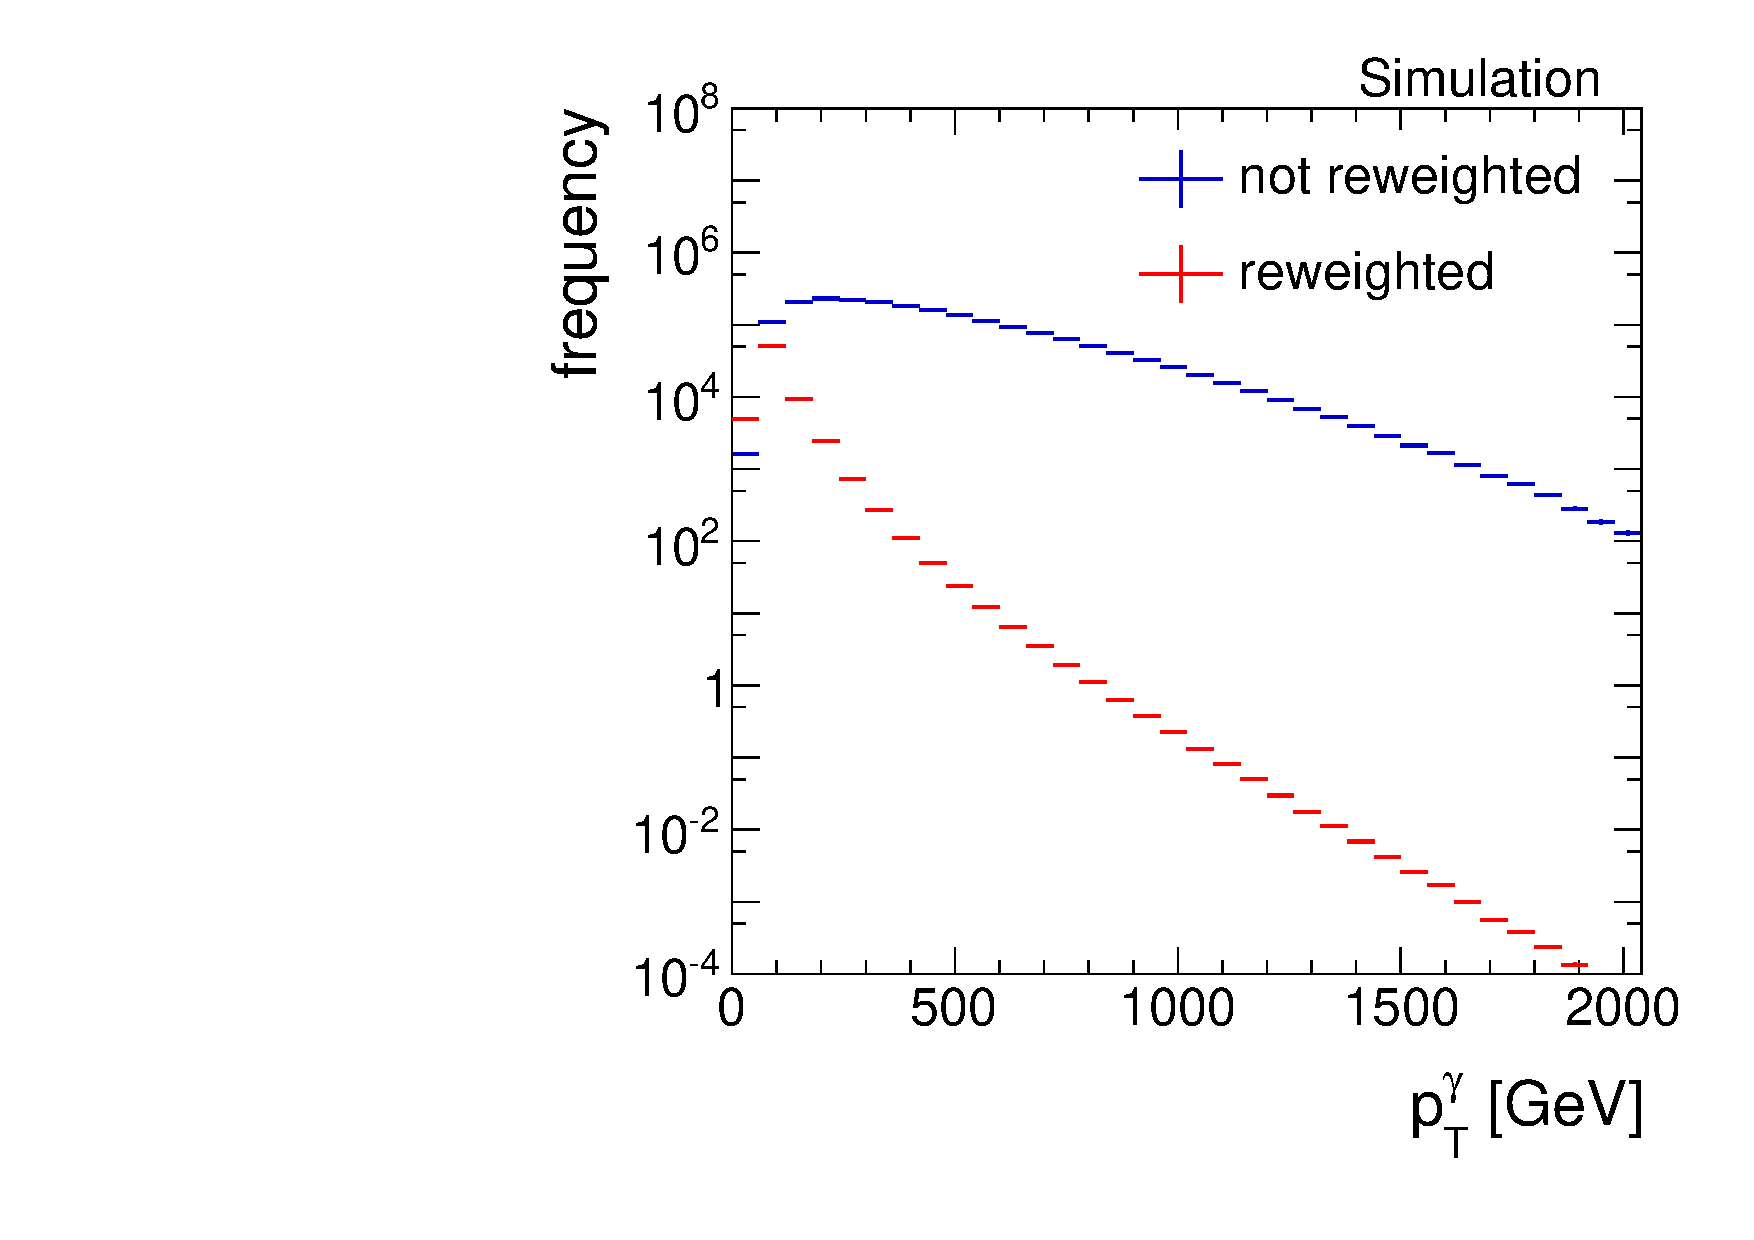
\includegraphics[width=0.49\textwidth]{figures/resolution/eventSelection/PhotonPtComparison_reweighted.pdf} 
  \caption{The photon \pt spectrum before (blue) and after (red) reweighing.}  
  \label{res:fig:PhotonPtSpectrum}
\end{figure}


\section{Event selection}
\label{res:sec:EventSelection}
Events are reconstructed with the particle-flow reconstruction algorithm, which uses information of all detector components to reconstruct individual particles~\cite{CMS-PAS-PFT-09-001}.
Furthermore, particles belonging to a jet are clustered with the Anti-k$_{\text{t}}$ jet clustering algorithm with a radius of R=0.5~\cite{Cacciari:2008gp}.

To select clean \GAMJET events, it is required that the leading jet meets the following requirements (these criteria correspond to a 'tight ID' in~\cite{website:JetIdentification,bib:CMS-AN-2010-003}):
\begin{itemize}

 \item Neutral hadron fraction $<$ 0.90
 \item Neutral electromagnetic fraction $<$ 0.90
 \item Number of constituents $>$ 1
\end{itemize}

 And for jets in the pseudorapidity range $|\eta^{\text{jet}}| < 2.4 $ :
\begin{itemize}
 \item Charged hadron fraction $>$ 0
 \item Charged hadron multiplicity $>$ 0
 \item Charged electromagnetic fraction $<$ 0.99
\end{itemize}
To mitigate effects from pileup, the first and second jet are required to have a transverse momentum greater 10\gev.

Concerning the photon, a maximal pseudorapidity of the photon of $|\eta^{\gamma}| < 1.3$ is demanded to exploit the high resolution of the ECAL in the barrel region.

Furthermore, the resolution is determined for different ranges in photon \pt to avoid mixing of different prescales of the various triggers. 
In Table~\ref{res:tab:PhotonPtBins} the applied binning is shown with the respective triggers contributing to each $\pt^{\gamma}$ bin.


\renewcommand{\arraystretch}{1.5}
\begin{table}[htb]
\centering
\caption{Photon \pt bins and corresponding triggers.}
\label{res:tab:PhotonPtBins}
\makebox[0.99\textwidth]{
\begin{tabular}{lc}
\multicolumn{2}{c}{} \\
\toprule
$\pt^{\gamma}$-bins           & Trigger         \\
\midrule
22\gev    & HLT\_Photon20\_CaloIdVL\_IsoL\_v* \\
36\gev    & HLT\_Photon30\_CaloIdVL\_IsoL\_v* \\
60\gev    & HLT\_Photon50\_CaloIdVL\_IsoL\_v* \\
88\gev    & HLT\_Photon75\_CaloIdVL\_IsoL\_v* \\
105\gev   & HLT\_Photon90\_CaloIdVL\_IsoL\_v* \\
149\gev   & HLT\_Photon135\_v*                \\
165\gev   & HLT\_Photon150\_v*                \\
\bottomrule
\multicolumn{2}{c}{} \\
\end{tabular}}
\end{table}

QCD multijets events constitute an important background to the \GAMJET events: A photon can be faked by a $\pi^{0}$ decaying into two close-by photons. 
Therefore, a very clean selection of the photons is necessary to suppress this background.
The following variables are used (see~\cite{CMS-PAS-EGM-10-006} for further explanation of the variables):

\begin{itemize}
 \item $\frac{\textbf{H}}{\textbf{E}}$ : The ratio of the measured energy in the hadronic calorimeter over the energy measured in the electromagnetic calorimeter. 
                                                    For photons, this is supposed to be very small as they deposit their energy predominantly in the ECAL.
 \item $\mathbold{\sigma_{i\eta i \eta}}$: The energy weighted spatial width of the photon energy deposition. The electromagnetic shower of a photon has a small lateral size 
                                           resulting in small $\sigma_{i\eta i \eta}$ for prompt photons while showers from fake photons, \eg $\pi^{0} \rightarrow \gamma \gamma$
                                           have a larger lateral size.
 \item \textbf{Jurassic ECAL isolation}: This isolation criterion uses the information of reconstructed hits ``RecHits'' (coming from the local reconstruction of the digital signals) 
                                         in a cone around the photon supercluster of R=0.4. Those are summed up and an upper criterion is identified to discriminate against 
                                         background which is typically spatially broader.  
 \item \textbf{Tower-based HCAL isolation}: The isolation criterion requires the energy deposited in all HCAL towers around the photon in cone of R=0.4 to be small compared to the 
                                            photon's energy. 
 \item \textbf{Hollow cone track isolation}: Requires absence of high-energetic tracks around the photon.
 \item \textbf{Pixel seed veto}: In order to reduce the background from electrons and positrons, the absence of a pixel-seed in the pixel tracker along the photons 
                                 trajectory is required.
\end{itemize}

The upper and lower bounds that are set on these observables can be found in Table~\ref{res:tab:PhotonIsolation}. 
\renewcommand{\arraystretch}{1.5}
\begin{table}[htb]
\centering
\caption{Upper and lower bounds for all photon isolation criteria in the barrel $\left( |\eta^{\gamma}|<1.4442 \right)$.}
\label{res:tab:PhotonIsolation}
\makebox[0.99\textwidth]{
\begin{tabular}{lc}
\multicolumn{2}{c}{} \\
\toprule
                              & Barrel                          \\
\midrule
$\frac{\text{H}}{\text{E}}$   & $<$ 0.05                        \\
$\sigma_{i\eta i \eta}$           & $<$ 0.013                       \\
ECAL isolation                & $<4.2 + 0.0060 \cdot \pt^{\gamma}$   \\
HCAL isolation                & $<2.2 + 0.0025 \cdot \pt^{\gamma}$   \\
Track Isolation               & $<2.0 + 0.0010 \cdot \pt^{\gamma}$   \\
Pixel seed veto               & yes                              \\
\bottomrule
\multicolumn{2}{c}{} \\
\end{tabular}}
\end{table}
%\begin{table}[bt]
%\caption{Upper and lower bounds for all photon isolation criteria in the barrel $\left( |\eta^{\gamma}|<1.4442 \right)$ and endcap $\left(1.4442 <|\eta^{\gamma}|<2.5 \right)$ .}
%\renewcommand{\arraystretch}{1.5}
%\begin{center}
%\begin{tabular}{ l| c | c |}
%                              & Barrel                                  & Endcap                                  \\\hline
%$\frac{\text{H}}{\text{E}}$   & $<$ 0.05                                & $<$ 0.05                                \\\hline
%$\sigma_{i\eta i \eta}$       & $<$ 0.013                               & $<$ 0.03                                \\\hline
%ECAL isolation                & $<4.2 + 0.0060 \, \pt^{\gamma}$   & $<4.2 + 0.0060 \, \pt^{\gamma}$    \\\hline
%HCAL isolation                & $<2.2 + 0.0025 \, \pt^{\gamma}$   & $<2.2 + 0.0025 \, \pt^{\gamma}$   \\\hline
%Track Isolation               & $<2.0 + 0.0010 \, \pt^{\gamma}$   & $<2.0 + 0.0010 \, \pt^{\gamma}$    \\\hline
%Pixel seed veto               & yes                                     & yes                                     \\\hline
%\end{tabular}
%\end{center}
%\label{tab:PhotonIsolation}
%\end{table}


Besides the mentioned requirements concerning the objects' attributes, two further criteria related to the event topology are crucial for this analysis:\\
An upper threshold on $\Delta \Phi$ between the leading jet and the photon and a maximal value for $\alpha$
\begin{itemize}
 \item $\Delta \Phi \left(\text{1st jet}, \gamma \right) > 2.95\,\unit{rad}$
 \item $\frac{\pt^{\text{2nd jet}}}{\pt^{\gamma}} < 0.20$.
\end{itemize}
These requirements are important to suppress events with too much further hadronic activity.

A summary of all selection criteria can be found in Appendix~\ref{res:app:eventselection}.
%%%%%%%%%%%%%%%%%%%%%%%%%%%%%%%%%%%%%%%%%%%%%%%%%%%%%%%%%%%%%%%%%%%%%%%%%%%%%%%%%%%%%%%%%%%%%%%%%%%%%%%%%%%%%%%%%%%%%%%%%%%%%%%%%%%%%%%%%%%%%%%%%%%%%%%%%%%%%%%%%%%%%%%%%%%%%%%%%%%%%%%%%%%%%%%%%%%%%%%%%%%%%%%%%%%%%%%%%%%%%%%%%%%%%%%%%%%

%%%%%%%%%%%%%%%%%%%%%%%%%%%%%%%%%%%%%%%%%%%%%%%%%%%%%%%%%%%%%%%%%%%%%%%%%%%%%%%%%%%%%%%%%%%%%%%%%%%%%%%%%%%%%%%%%%%%%%%%%%%%%%%%%%%%%%%%%%%%%%%%%%%%%%%%%%%%%%%%%%%%%%%%%%%%%%%%%%%%%%%%%%%%%%%%%%%%%%%%%%%%%%%%%%%%%%%%%%%%%%%%%%%%%%%%%%%
%%%%%%%%%%%%%%%%%%%%%%%%%%%%%%%%%%%%%%%%%%%%%%%%%%%%%%%%%%%%%%%%%%%%%%%%%%%%%%%%%%%%%%%%%%%%%%%%%%%%%%%%%%%%%%%%%%%%%%%%%%%%%%%%%%%%%%%%%%%%%%%%%%%%%%%%%%%%%%%%%%%%%%%%%%%%%%%%%%%%%%%%%%%%%%%%%%%%%%%%%%%%%%%%%%%%%%%%%%%%%%%%%%%%%%%%%%%
\FloatBarrier
\chapter{Methodology of the measurement}
%\interfootnotelinepenalty=10000

The basic methodology of measuring the jet transverse-momentum resolution by exploiting the \pt balance in $\GAMJET$ events and extrapolating the result to small $\alpha$ that was already used in earlier analyses~\cite{bib:CMS:JERCPaper_2011}, 
is extended in this measurment in order to explicitly distinguish the case of parton radiation in different event hemispheres.

As already described in Section~\ref{res:ch:GeneralApproach}, the idea behind a resolution measurement with $\GAMJET$ events is the usage of the photon energy instead of the true jet energy.
This results in a twofold contribution to the measured response, the intrinsic response and the imbalance:

\begin{equation}\label{eq:splittedResolution}
\frac{\ptrecojet}{\ptgamma} = \underbrace{\frac{\ptrecojet}{\ptgenjet}}_{\text{intrinsic}} \cdot \underbrace{\frac{\ptgenjet}{\ptgamma}}_{\text{imbalance}}.
\end{equation}

Taking the photon \pt as true jet \pt estimator instead of the generator jet \pt, and thus measuring the response defined as \ptrecojet/\ptgamma, results in a different shape of the response function as shown in Fig.~\ref{fig:responseExamples}. 
The figure compares the intrinsic response, the imbalance, and the measured total response in simulation. 

\begin{figure}[t]
 \centering
     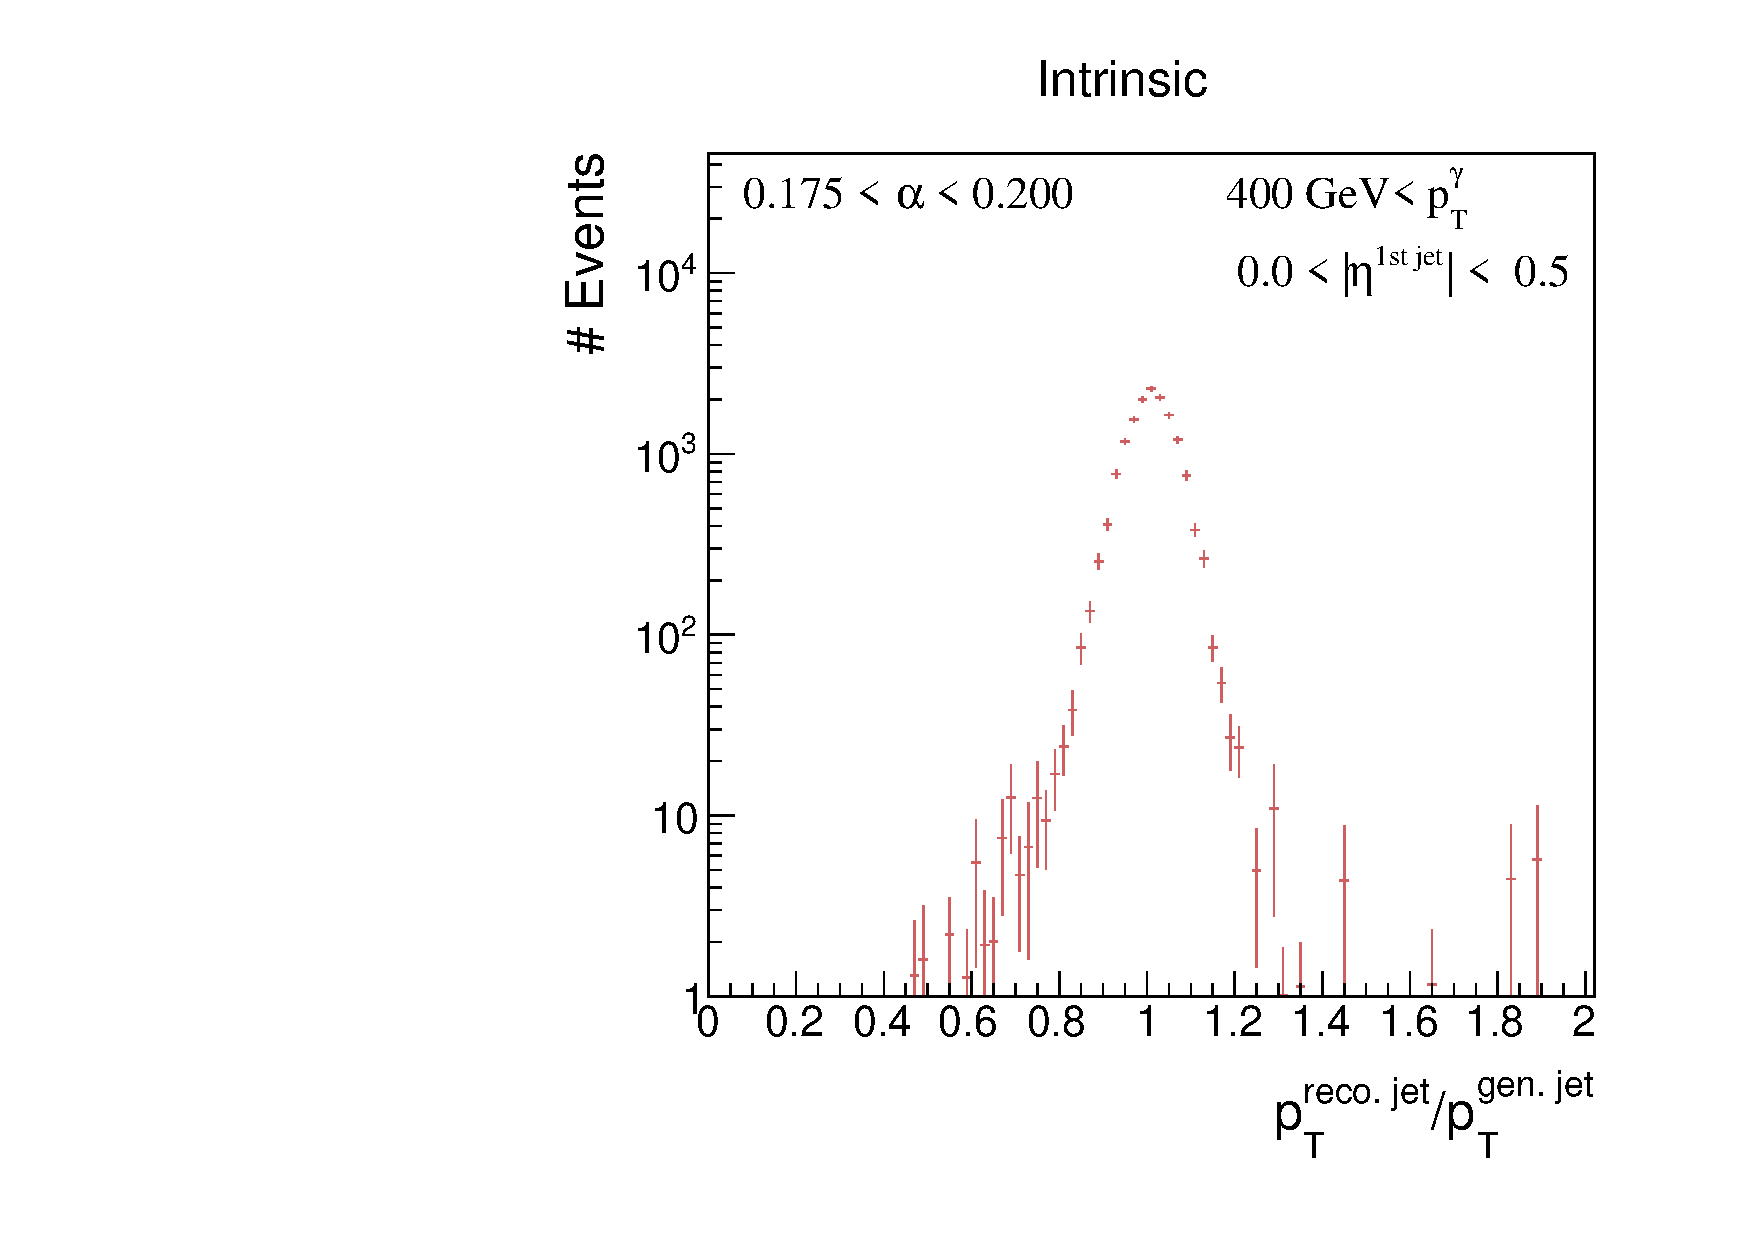
\includegraphics[width=0.49\textwidth]{figures/resolution/methodology/intrinsicExample.pdf}
     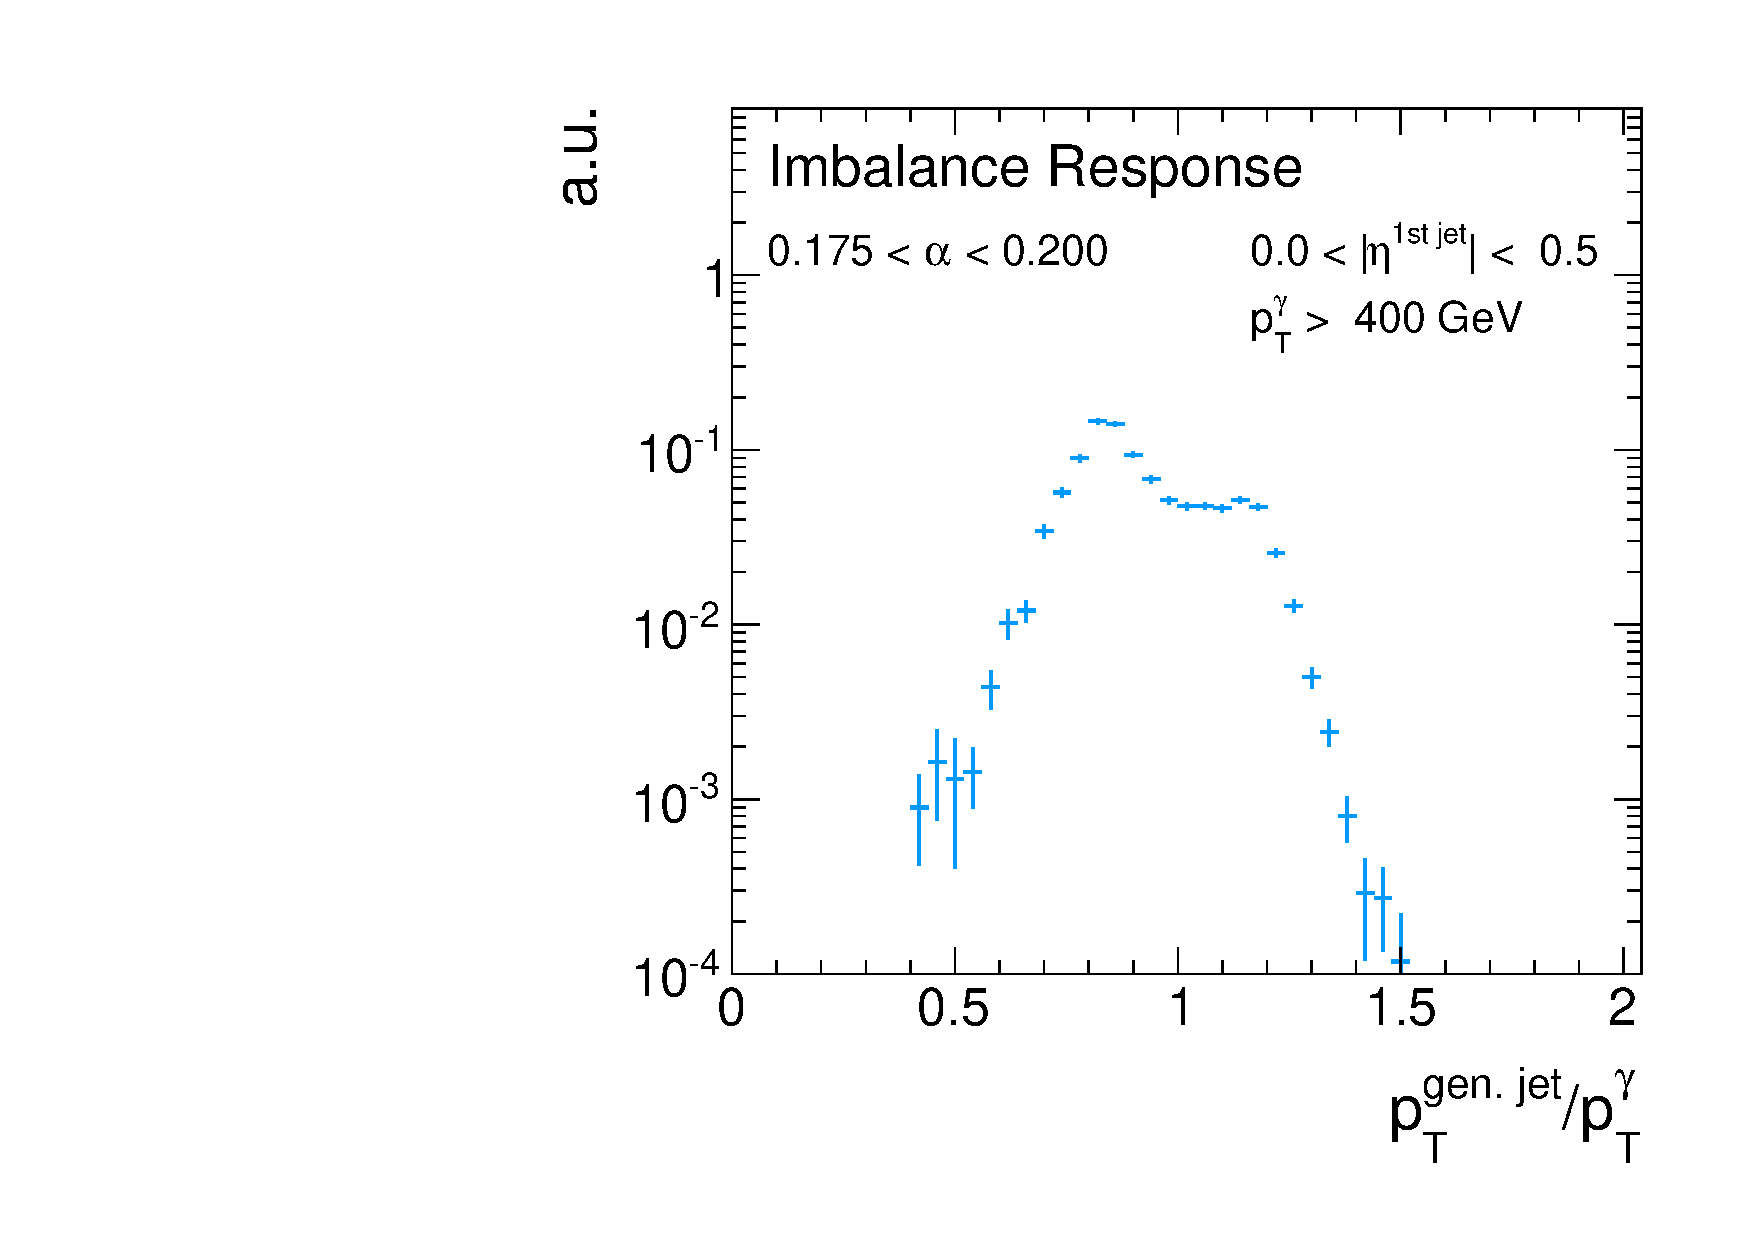
\includegraphics[width=0.49\textwidth]{figures/resolution/methodology/imbalanceExample.pdf}

     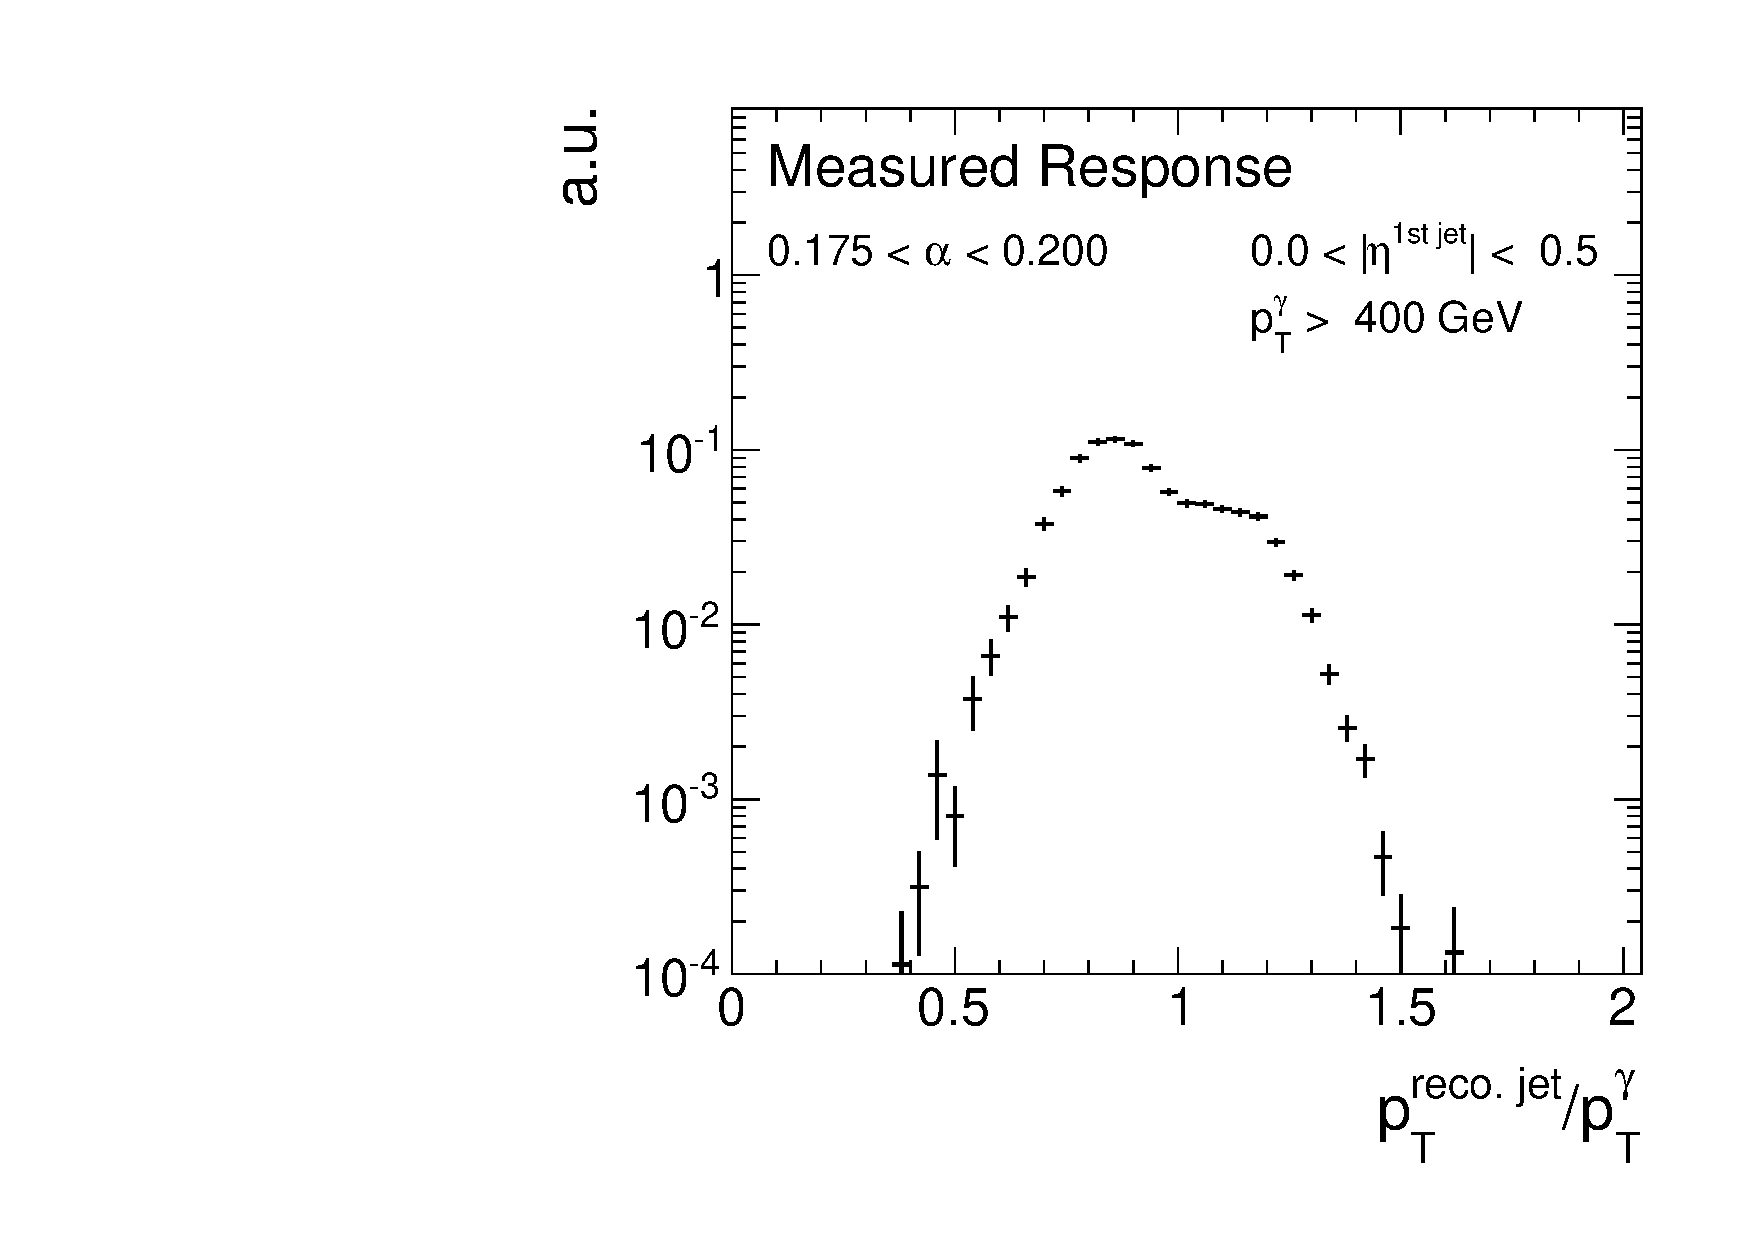
\includegraphics[width=0.49\textwidth]{figures/resolution/methodology/fullResponseExample.pdf}
  \caption{The two different contributions, intrinsic (top left) and imbalance (top right), to the measured response (bottom), 
           cf. \mbox{Eq.~\eqref{eq:splittedResolution}}, in simulated events.}  
 \label{fig:responseExamples}
\end{figure}


The clear difference between the intrinsic response and the imbalance is the double peak structure of the latter one. The measured response is a convolution of the two
contributions, where the double peak is consequentially less pronounced.

The occurrence of two peaks is caused by the hard selection in $\Delta \phi$ which forces the second jet to be either close to the photon or close to the leading jet 
due to \pt conservation. 
The possibility of an energetic second jet perpendicular to the leading jet-photon axis which is balanced by a third jet is very unlikely 
due to the decreasing jet multiplicity in QCD-multijet events.
The double peak structure is less pronounced for small second jet \pt (small $\alpha$) where the $\Delta \Phi$ requirement does not have such a strong effect in rejecting
events with a second jet perpendicular to the photon leading jet axis (see \mbox{Fig. \ref{fig:alphaBins}}).

\begin{figure}[bt]
 \centering
     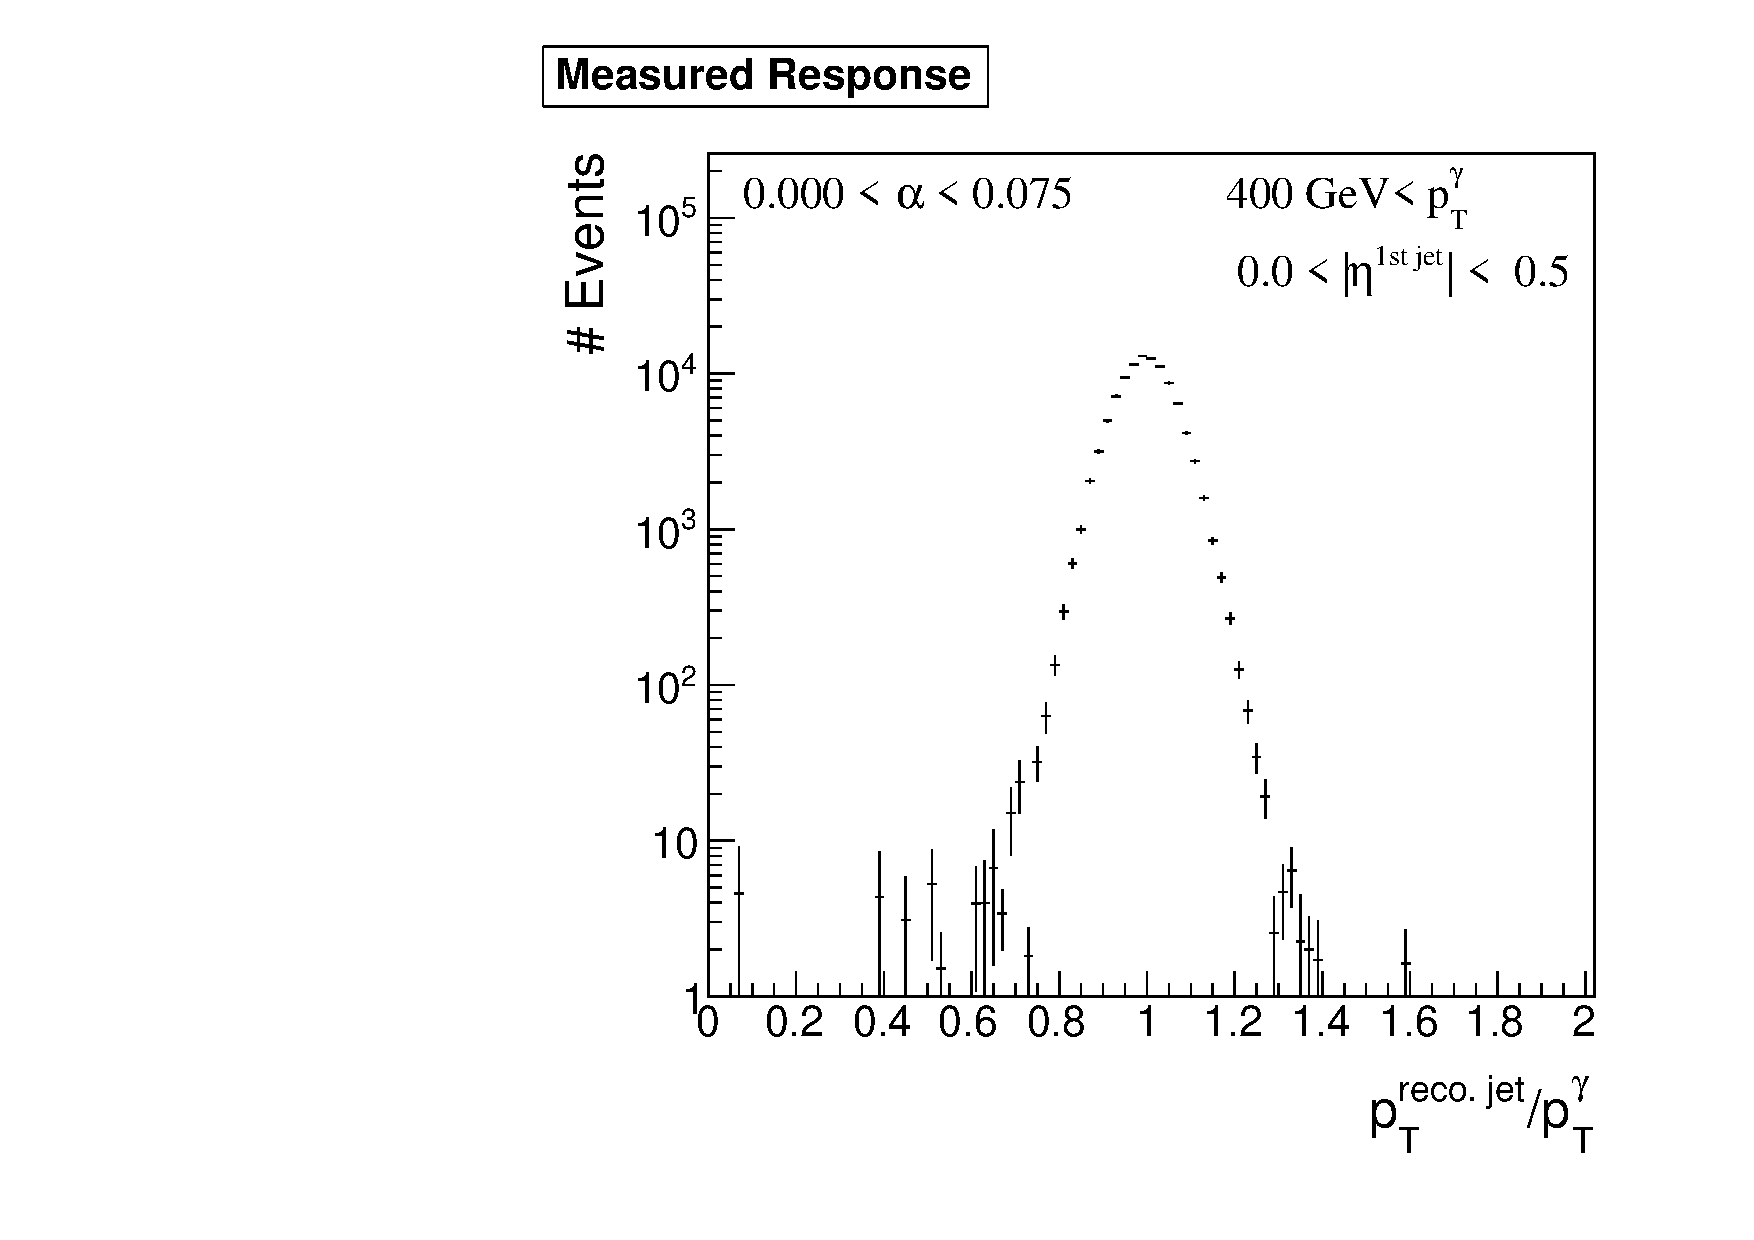
\includegraphics[width=0.33\textwidth]{figures/resolution/methodology/fullResponseExample1stBin.pdf}
     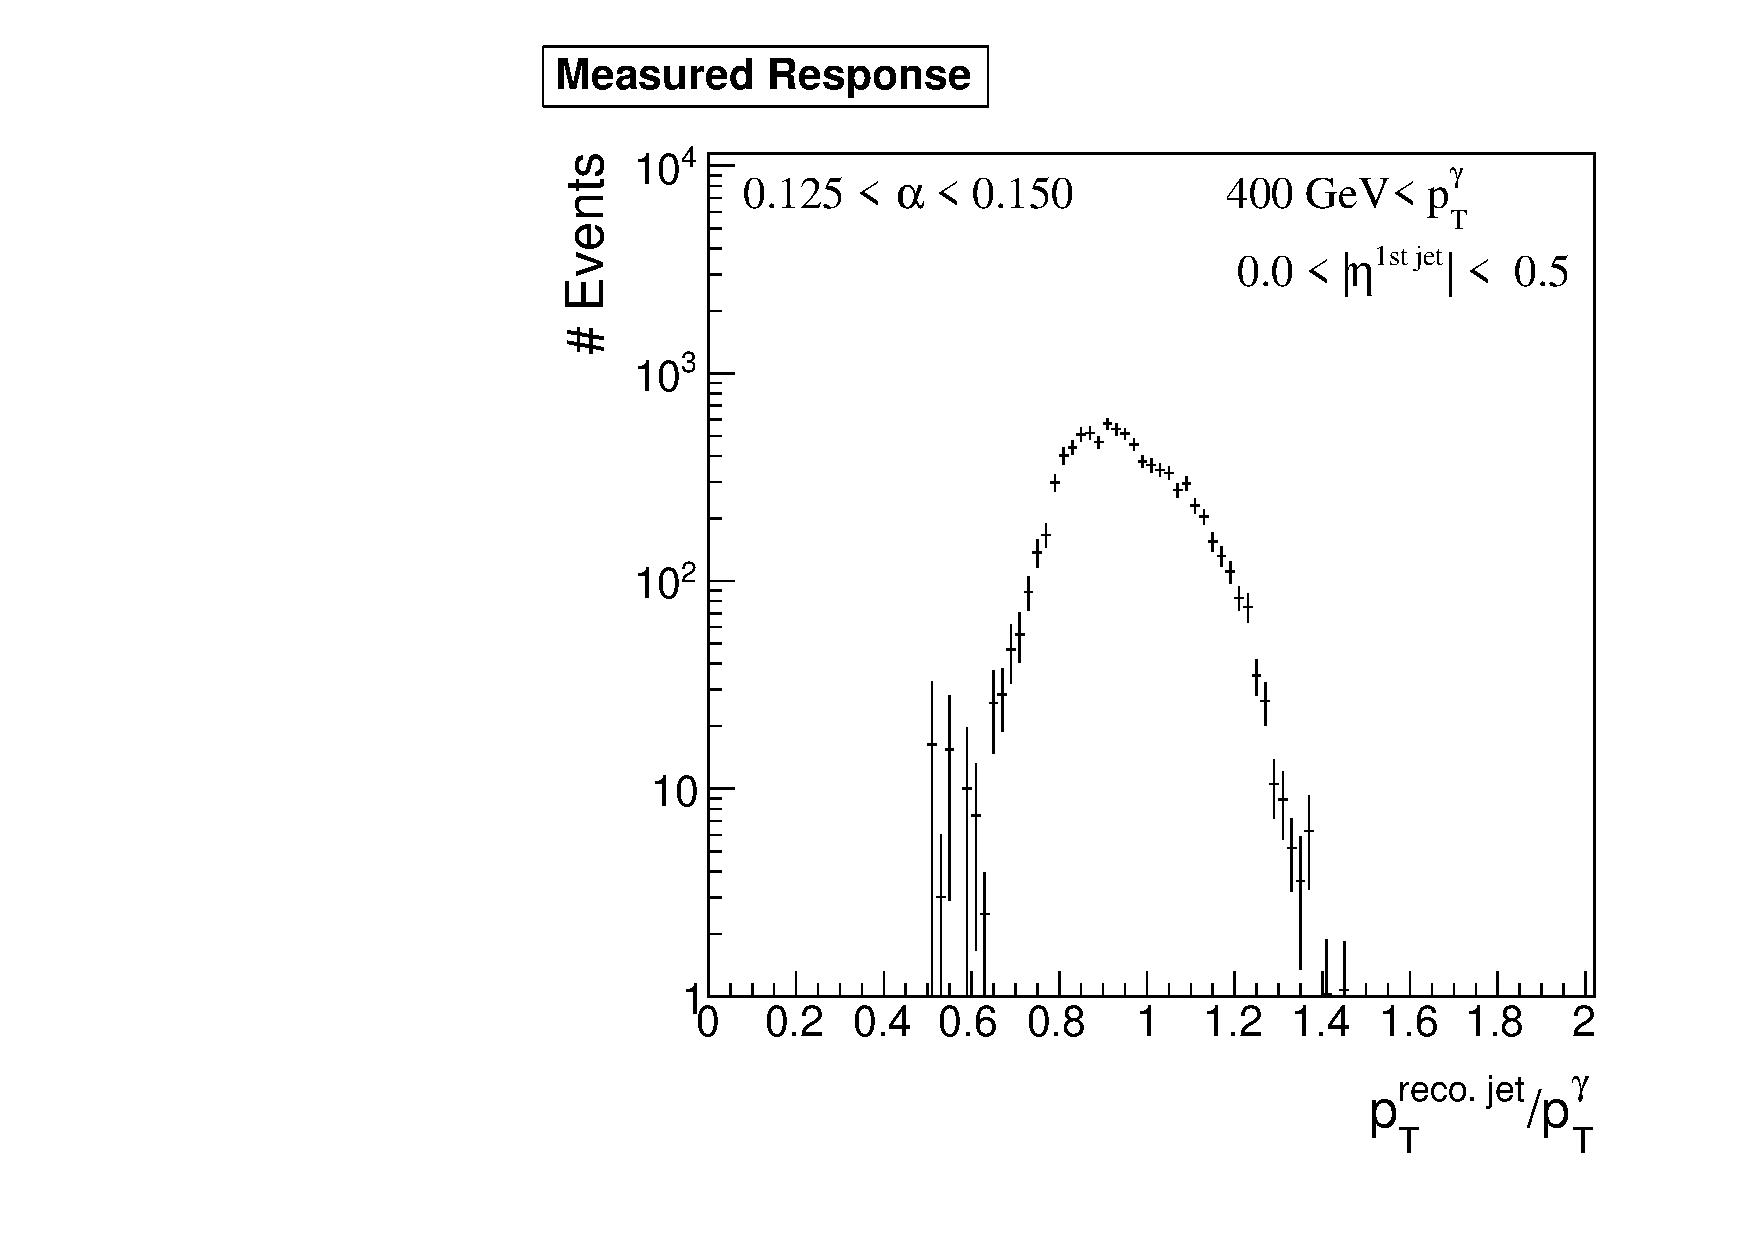
\includegraphics[width=0.33\textwidth]{figures/resolution/methodology/fullResponseExample4thBin.pdf}
     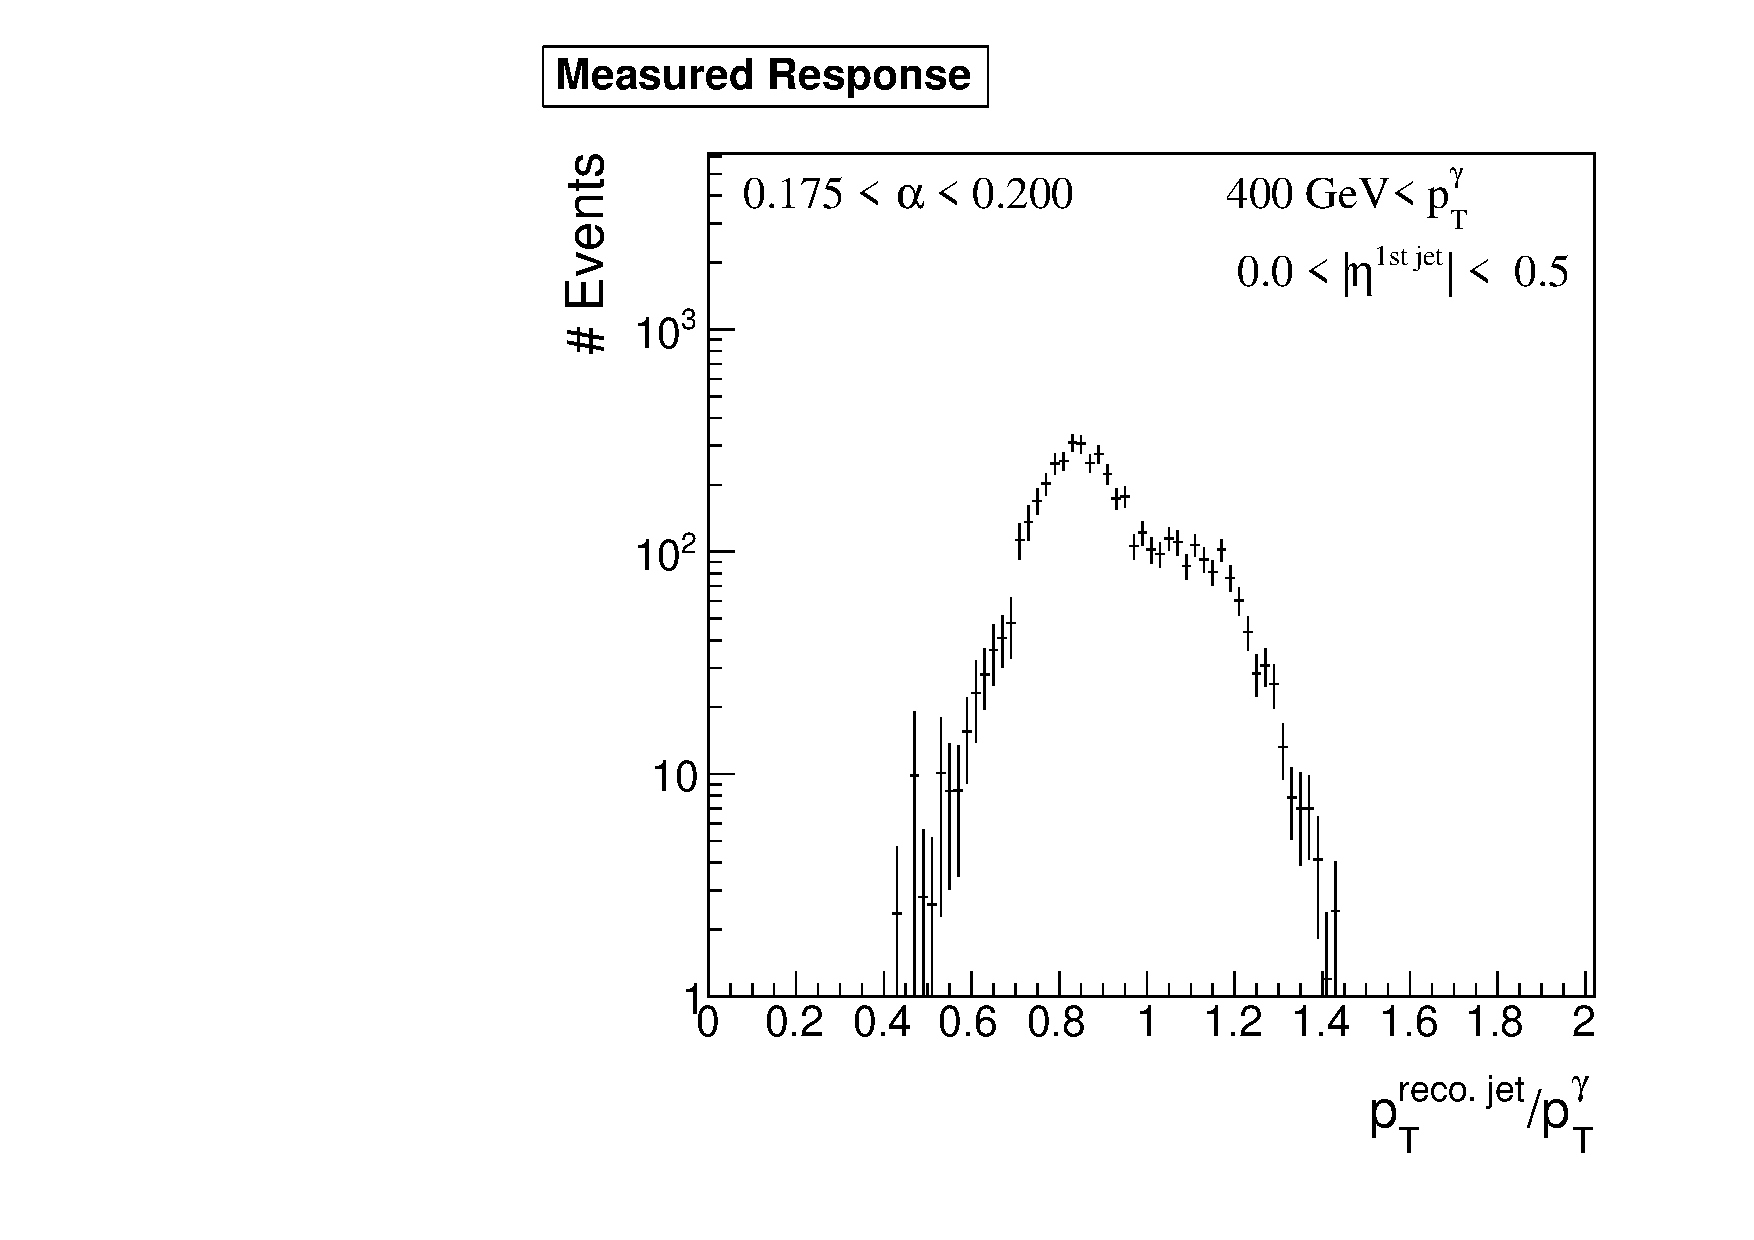
\includegraphics[width=0.33\textwidth]{figures/resolution/methodology/fullResponseExample6thBin.pdf}
  \caption{The measured response $\frac{\pt^{\text{reco. jet}}}{\pt^{\gamma}}$ in simulation for $\pt^{\gamma} < 400 \gev$ for three different $\alpha$ ranges: 
           (left) 0.0\%-7.5\%, (middle) 12.5\%-15.0\% and (right) 17.5\%-20.0 \%. 
           It can be seen that the double peak structure gets less pronounced for low $\alpha$ values.}  
 \label{fig:alphaBins}
\end{figure}

These two different contributions (second jet in photon/leading jet hemisphere) result in two separate response distribution.
A schematic sketch of the two contributions is shown in Fig.~\ref{fig:sketch}. 



The mathematical definitions of the hemispheres are as follows:
\begin{equation}\label{eq:HemisphereDefinition}
\text{Hemisphere} = \begin{cases}
  \text{Jet},    & \Delta \Phi \left( \text{\nth{1} jet,\,\nth{2} jet} \right) < \Delta \Phi \left( \gamma \text{, \nth{2} jet} \right) , \\
  \text{Photon}, & \text{else}.\\
\end{cases}
\end{equation}
The two response distributions coming from the different event topologies are separately evaluated. First, the resolution is determined for each of the configurations 
(cf. Fig.~\ref{fig:fullResponseAndContributions}), and then, the weighted mean of the two contributions is calculated.
\begin{figure}[!t]
 \centering
     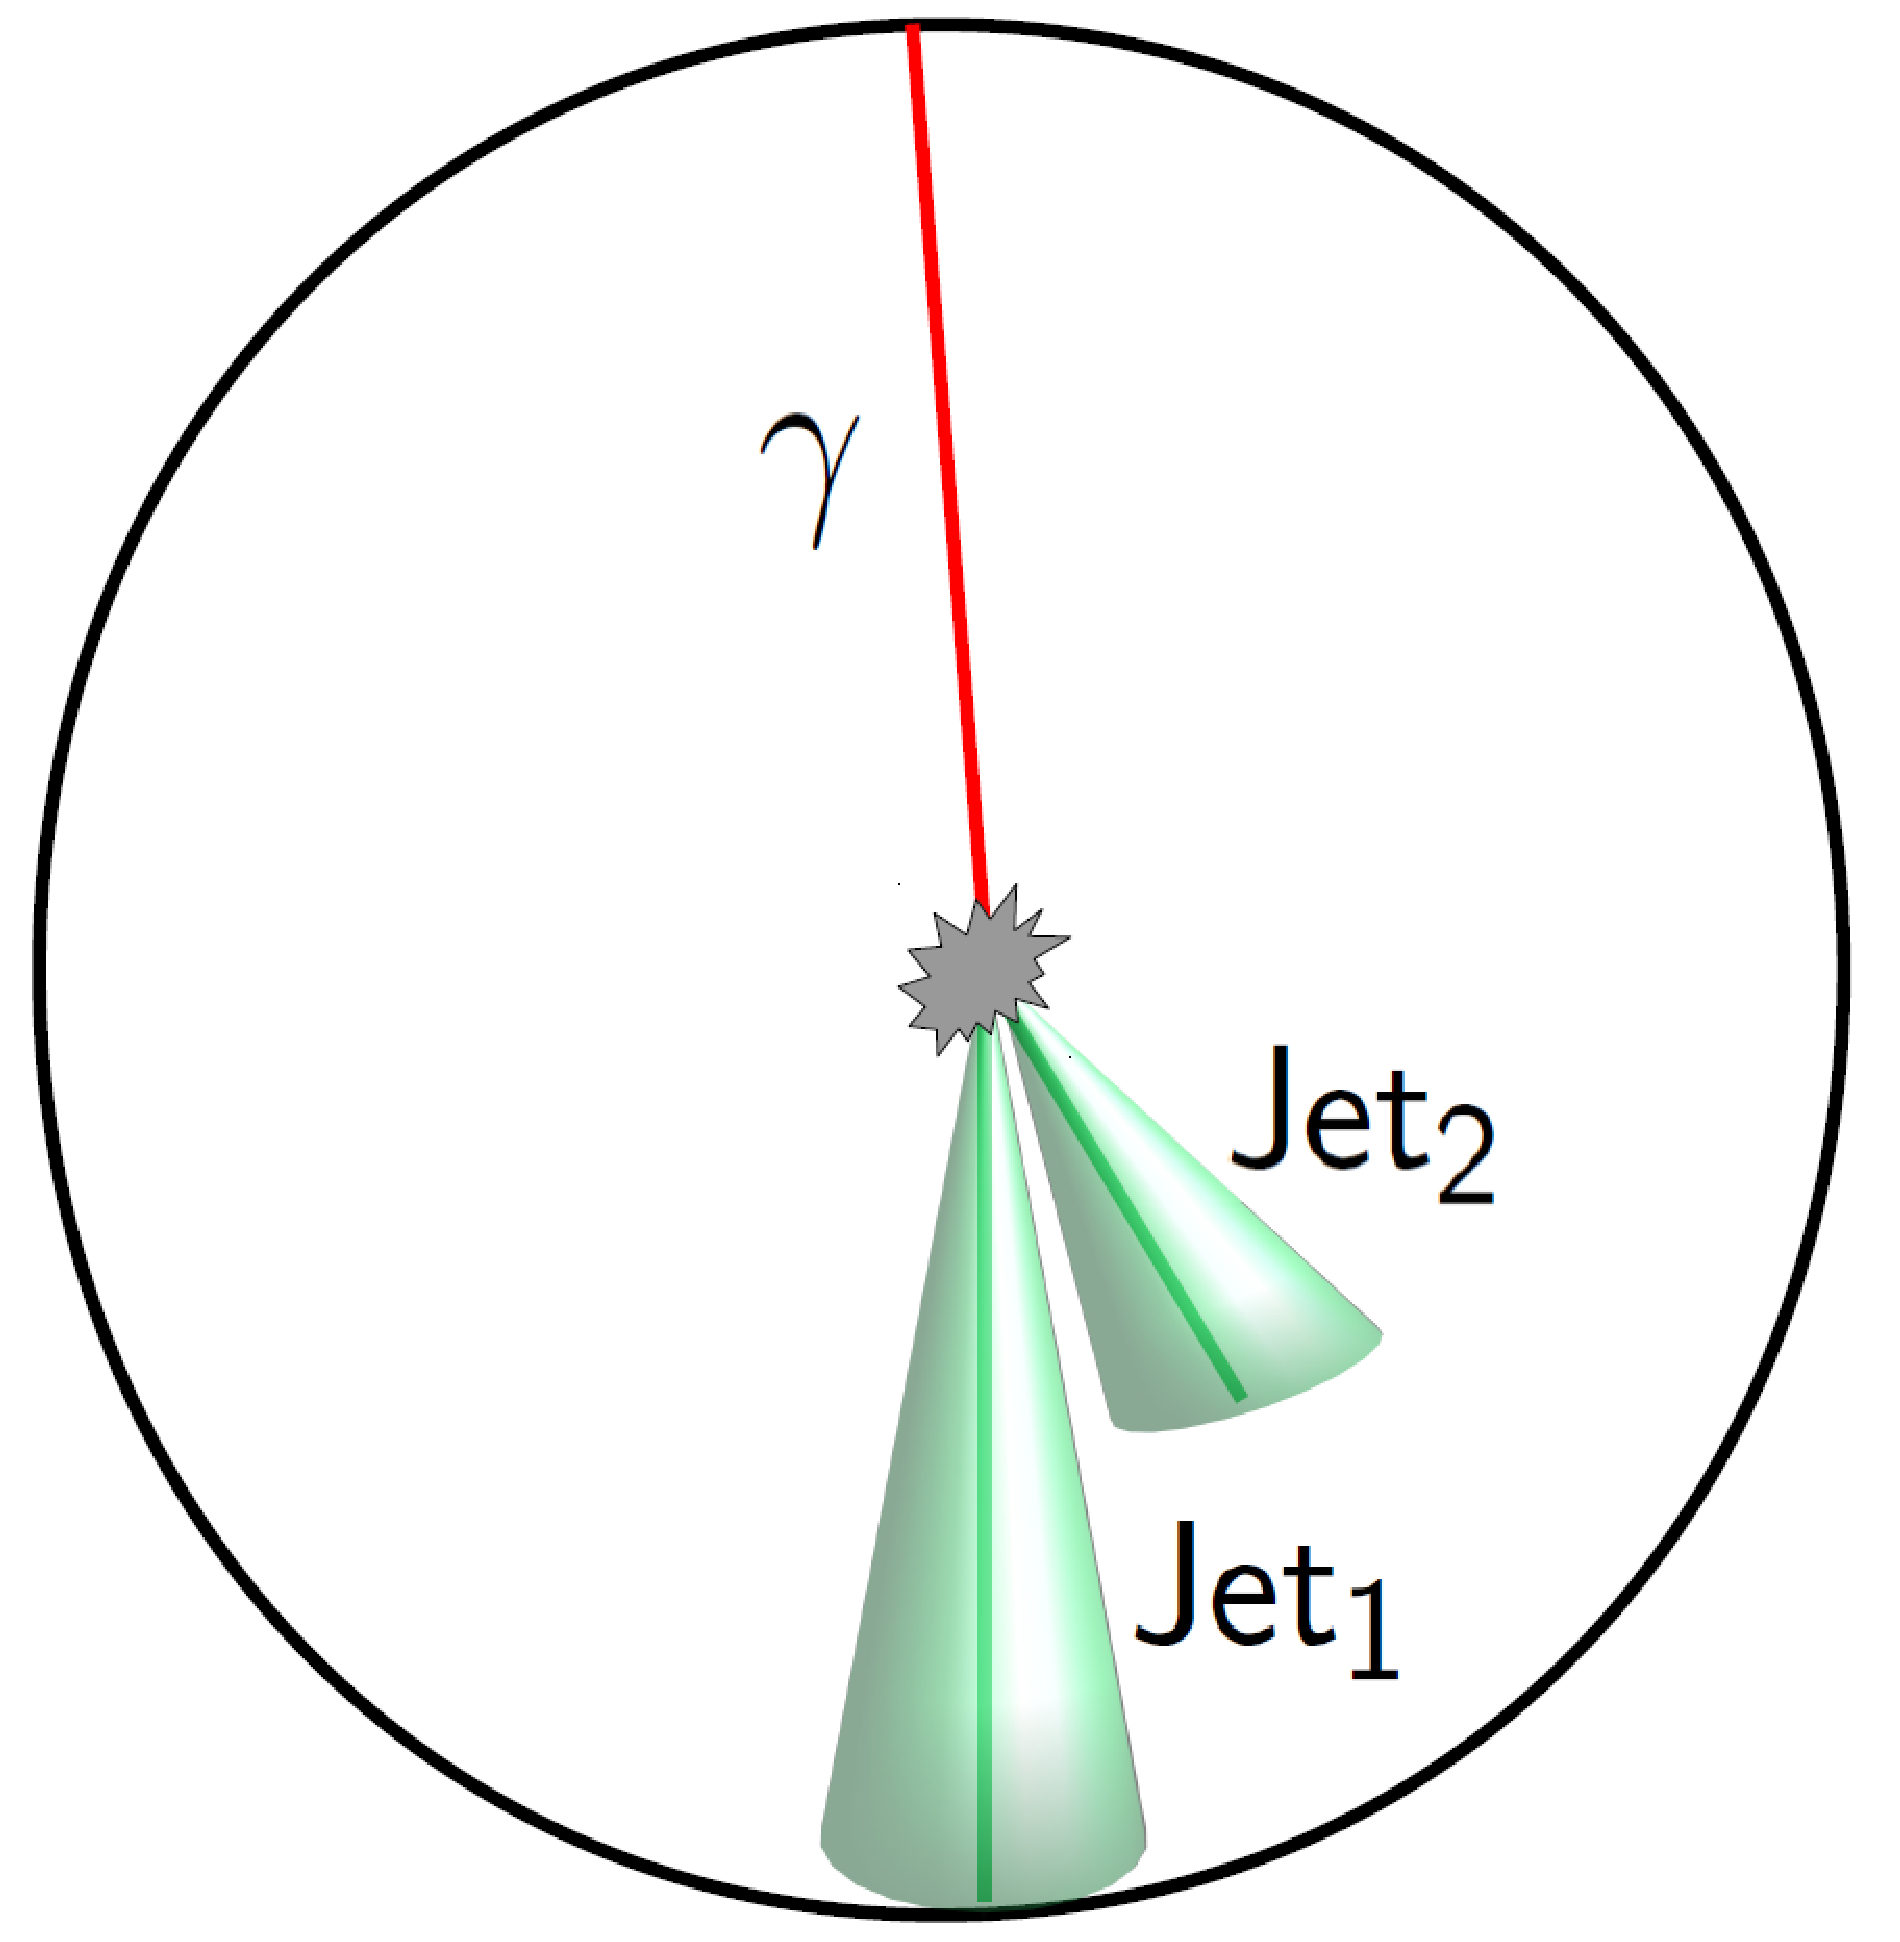
\includegraphics[width=0.49\textwidth]{figures/resolution/methodology/2ndJet_in_JetHemisphere.pdf}
     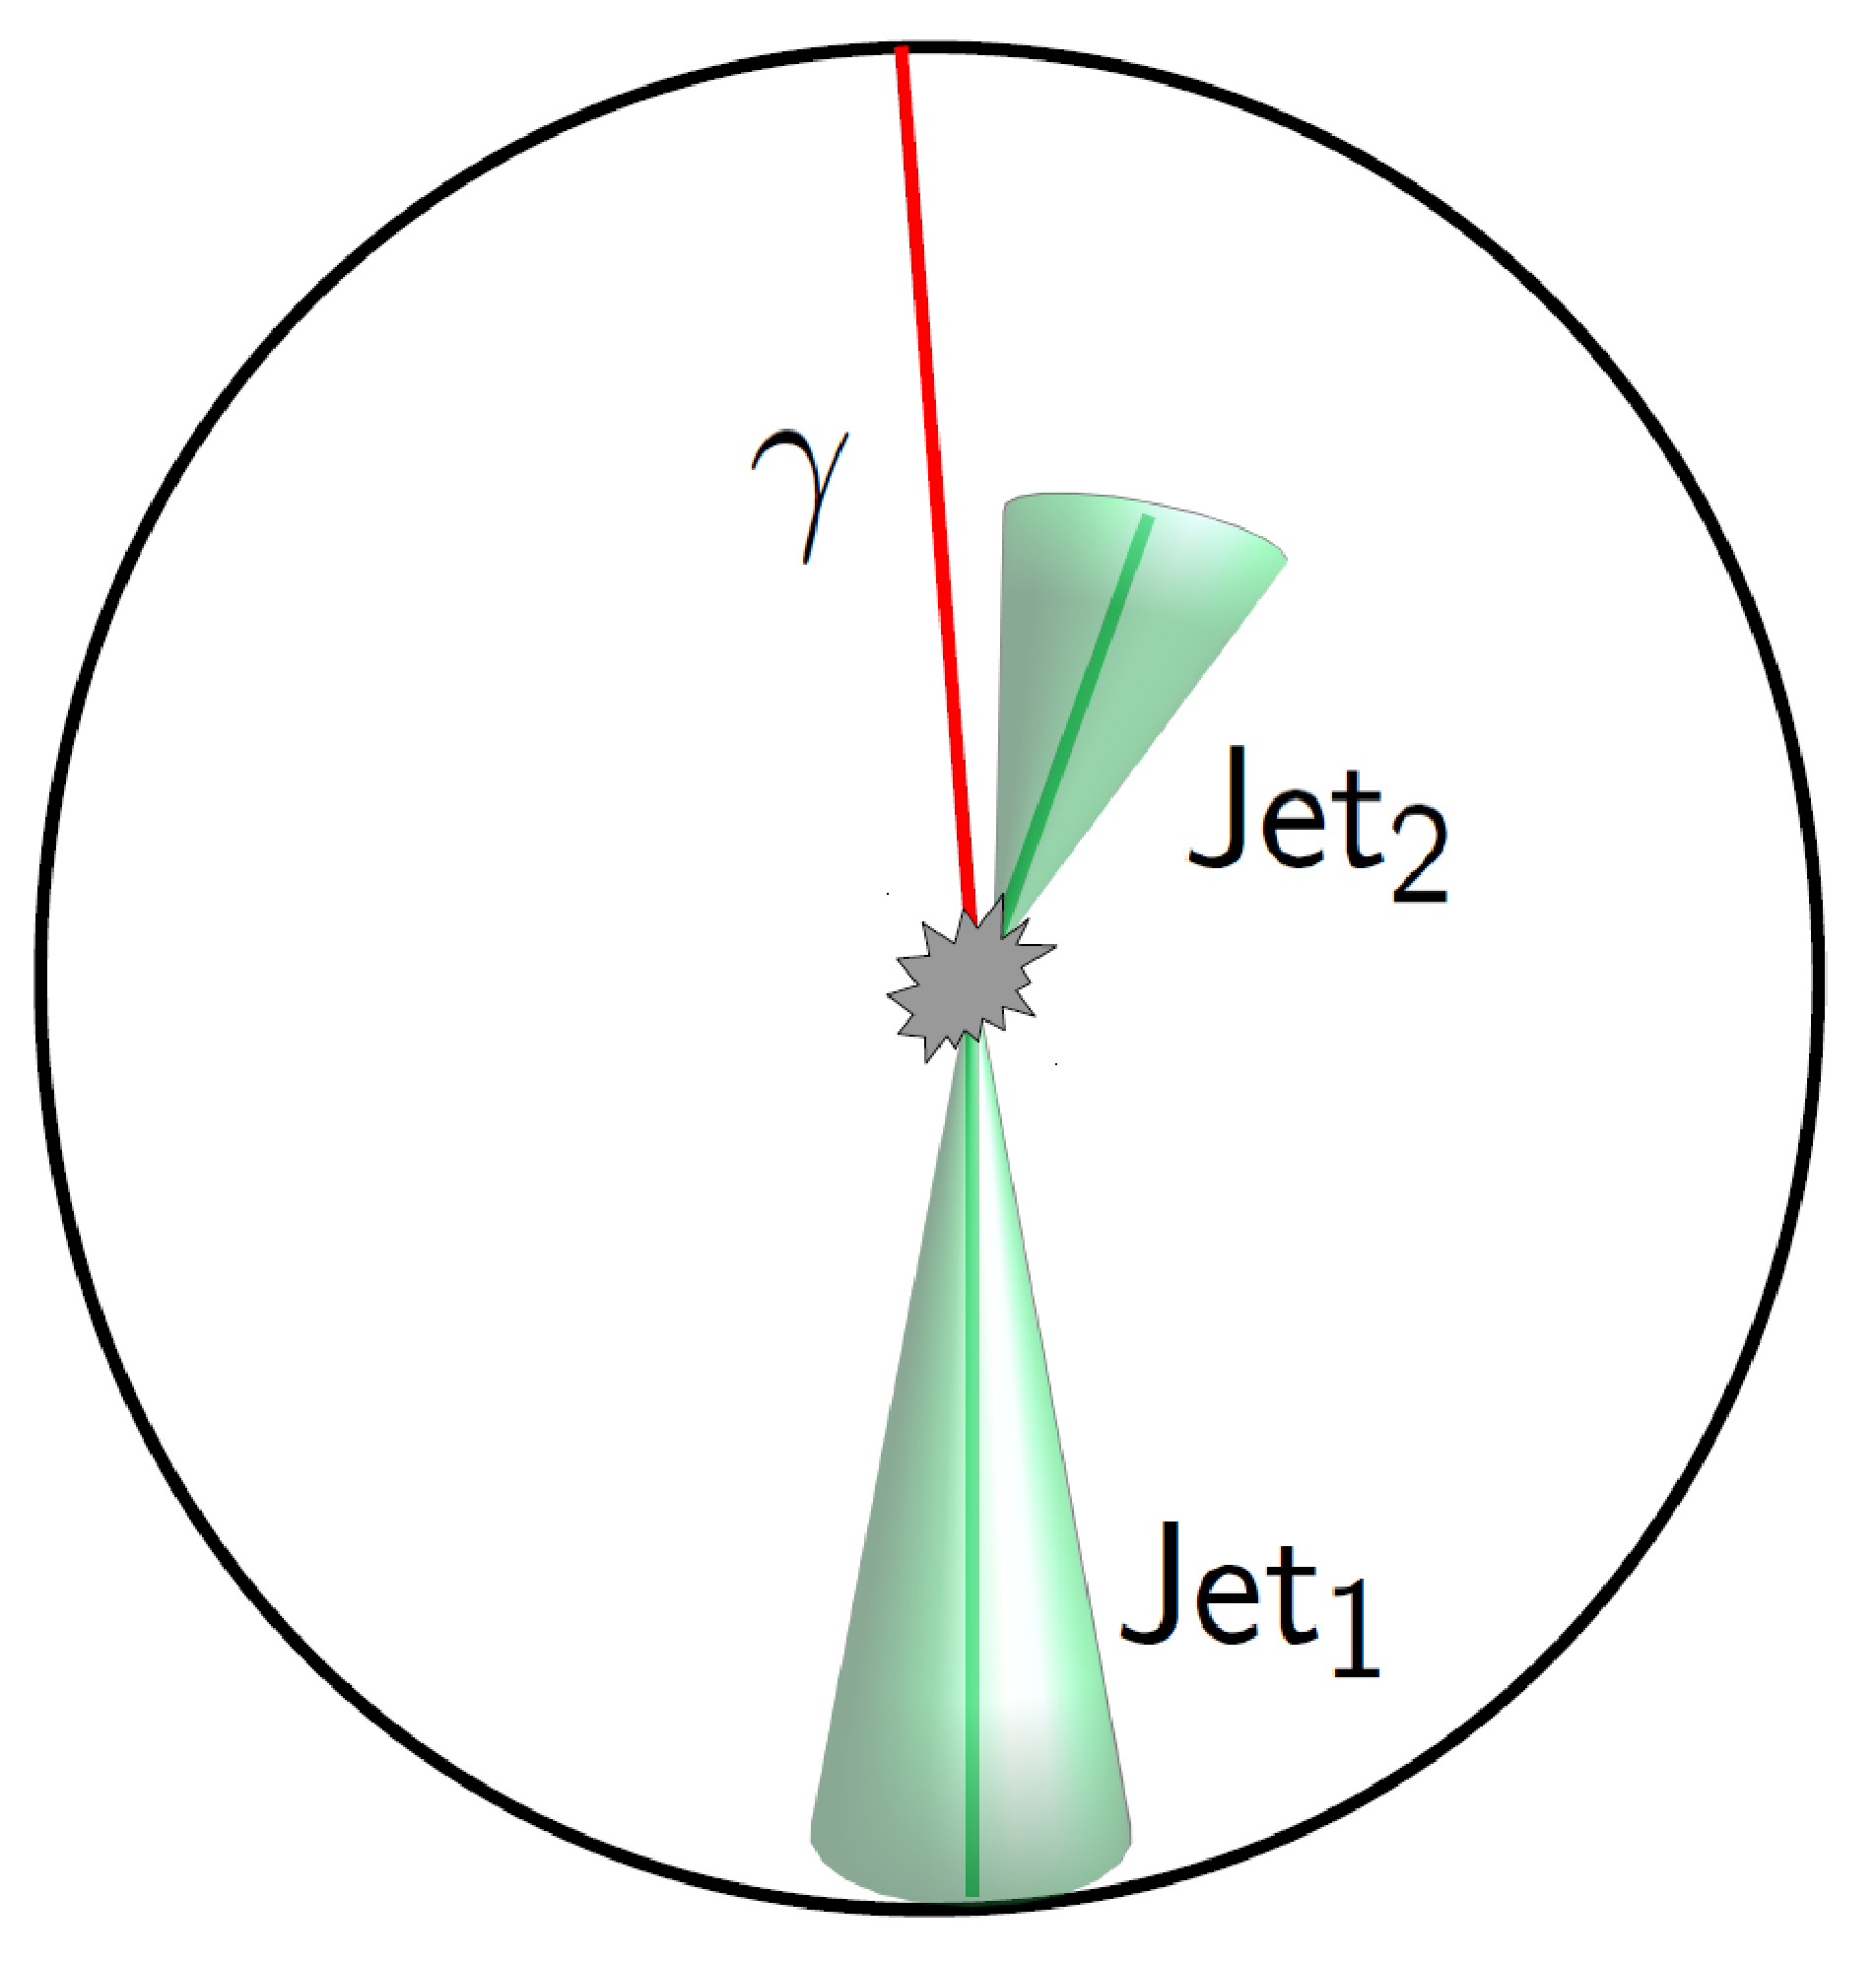
\includegraphics[width=0.49\textwidth]{figures/resolution/methodology/2ndJet_in_PhotonHemisphere.pdf}
  \caption{A schematic sketch of the two different event topologies where the second jet is in the leading jet (left) or the photon hemisphere (right)}  
 \label{fig:sketch}
\end{figure}
\begin{figure}[!b]
  \centering
  \vspace{35pt}
      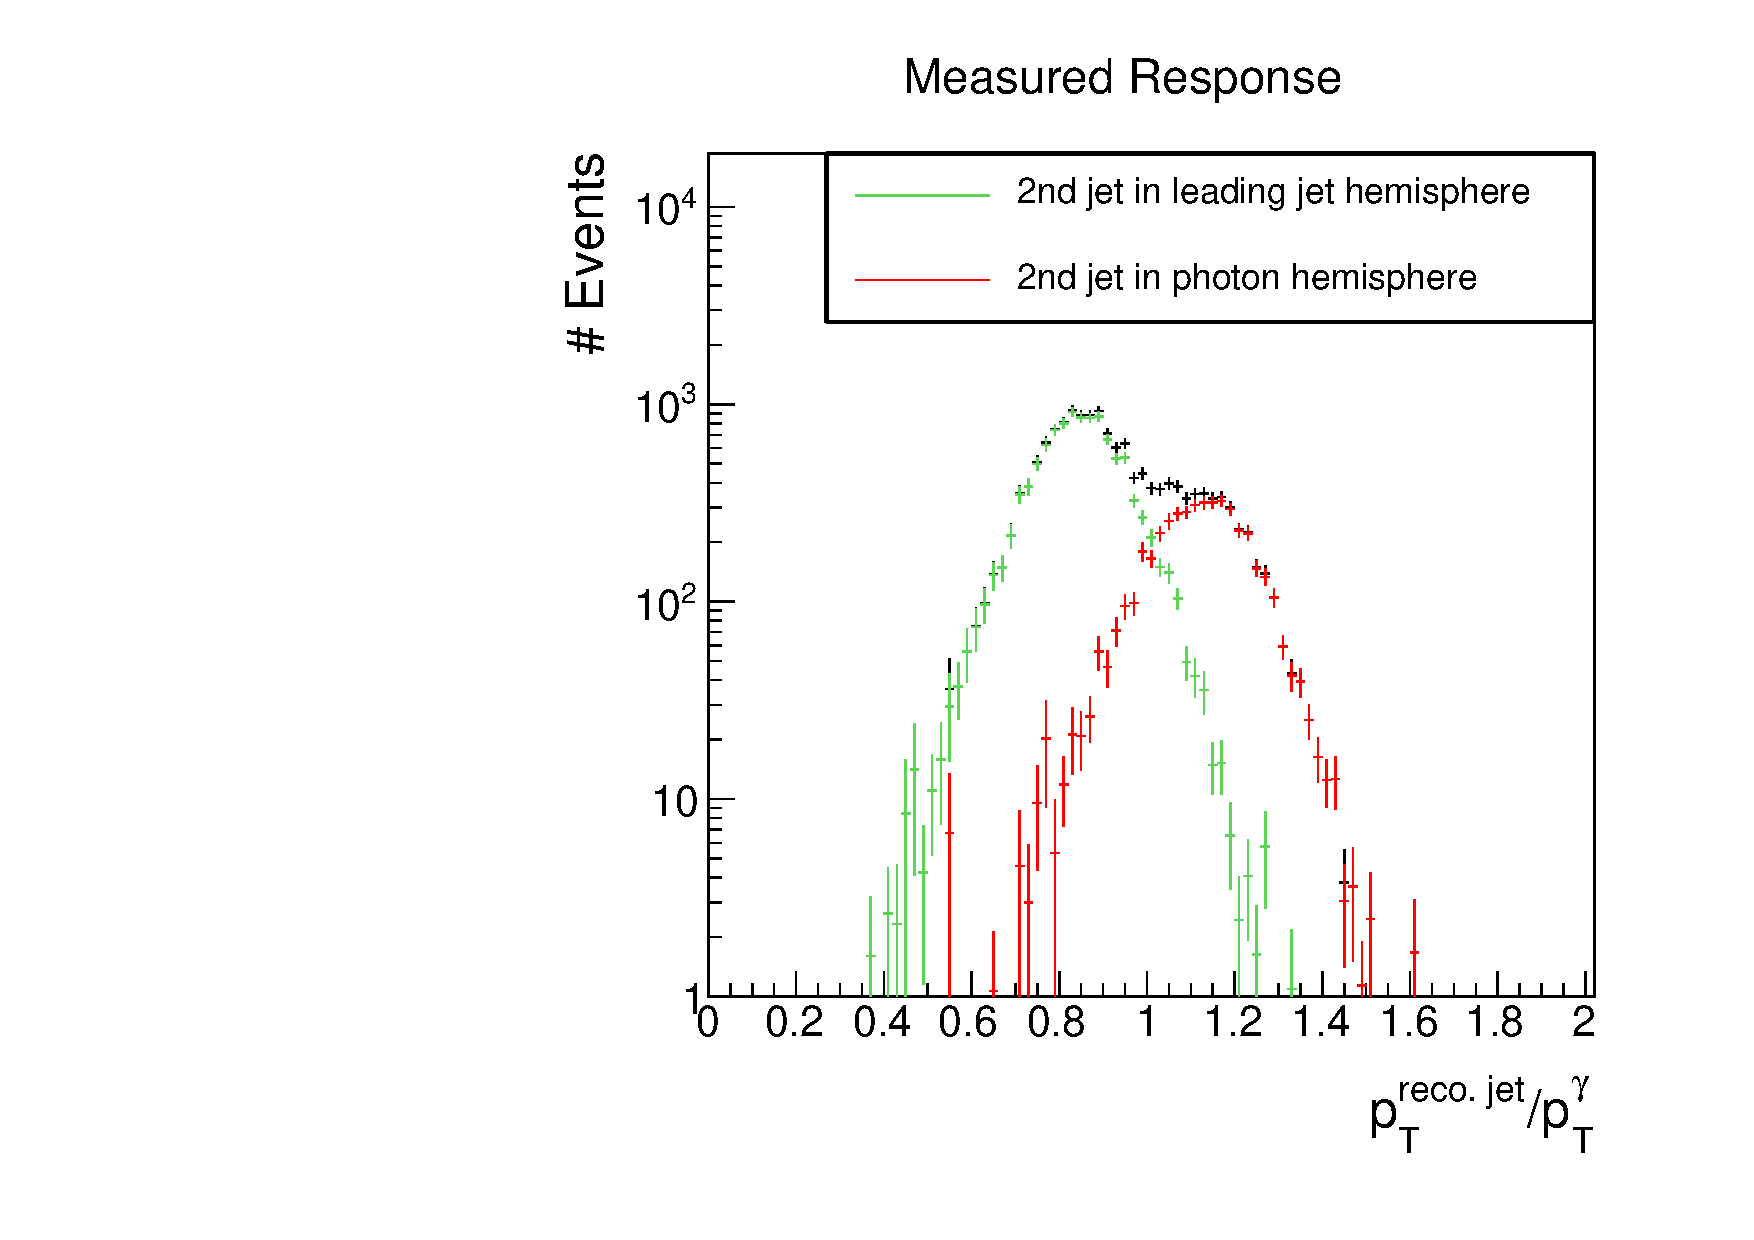
\includegraphics[width=0.49\textwidth]{figures/resolution/methodology/fullResponseAndContributionsExample.pdf}
  \caption{The measured response with the two contributions visualized. Events with a second jet in photon hemisphere (red) lead to a mean response larger one, while events with a
           second jet in the leading jet hemisphere (green) have a mean smaller one.}  
  \label{fig:fullResponseAndContributions}
\end{figure}

As can be seen in Fig.~\ref{fig:fullResponseAndContributions}, events containing a second jet in the leading jet hemisphere lead to a response histogram with mean smaller one, while events with a second jet in photon direction result in a distribution with mean larger one. 
The former occurs more frequently because it contains jets from final and initial state radiation, while the latter mainly consists only from initial state radiation.



The intrinsic part of the resolution for a given photon $\pt$ bin is independent of secondary jet energy and thus can be considered as a constant in terms of $\alpha$
\begin{equation}\label{eq:intrinsic}
 \jerintrinsic \left( \alpha\right) = c.
\end{equation}
This is not true for the imbalance part. It was found empirically that the $\alpha$ dependence of the imbalance can be described by a linear function 
\begin{equation}\label{eq:imbalance}
  \jerimbalance \left( \alpha\right) = q + m \cdot \alpha
\end{equation}
Considering these two contributions as independent and \fixme(maybe not correct) folding them,  $\jerintr\oplus\jerimb$ , result in the following formula of the total resolution
\begin{equation}\label{eq:total}
  \jertotal \left( \alpha \right) = \sqrt{ c^2 + q^2  + 2\, q\, m \cdot \alpha +m^2 \cdot \alpha^2}. 
\end{equation}
In Fig.~\ref{fig:AlphaDependenceOfResolutions}, the $\alpha$ dependence of the imbalance, the intrinsic resolution, and the total resolution is shown for two examplary \ptgamma regions in simulated events. 
\begin{figure}[!b]
 \centering
    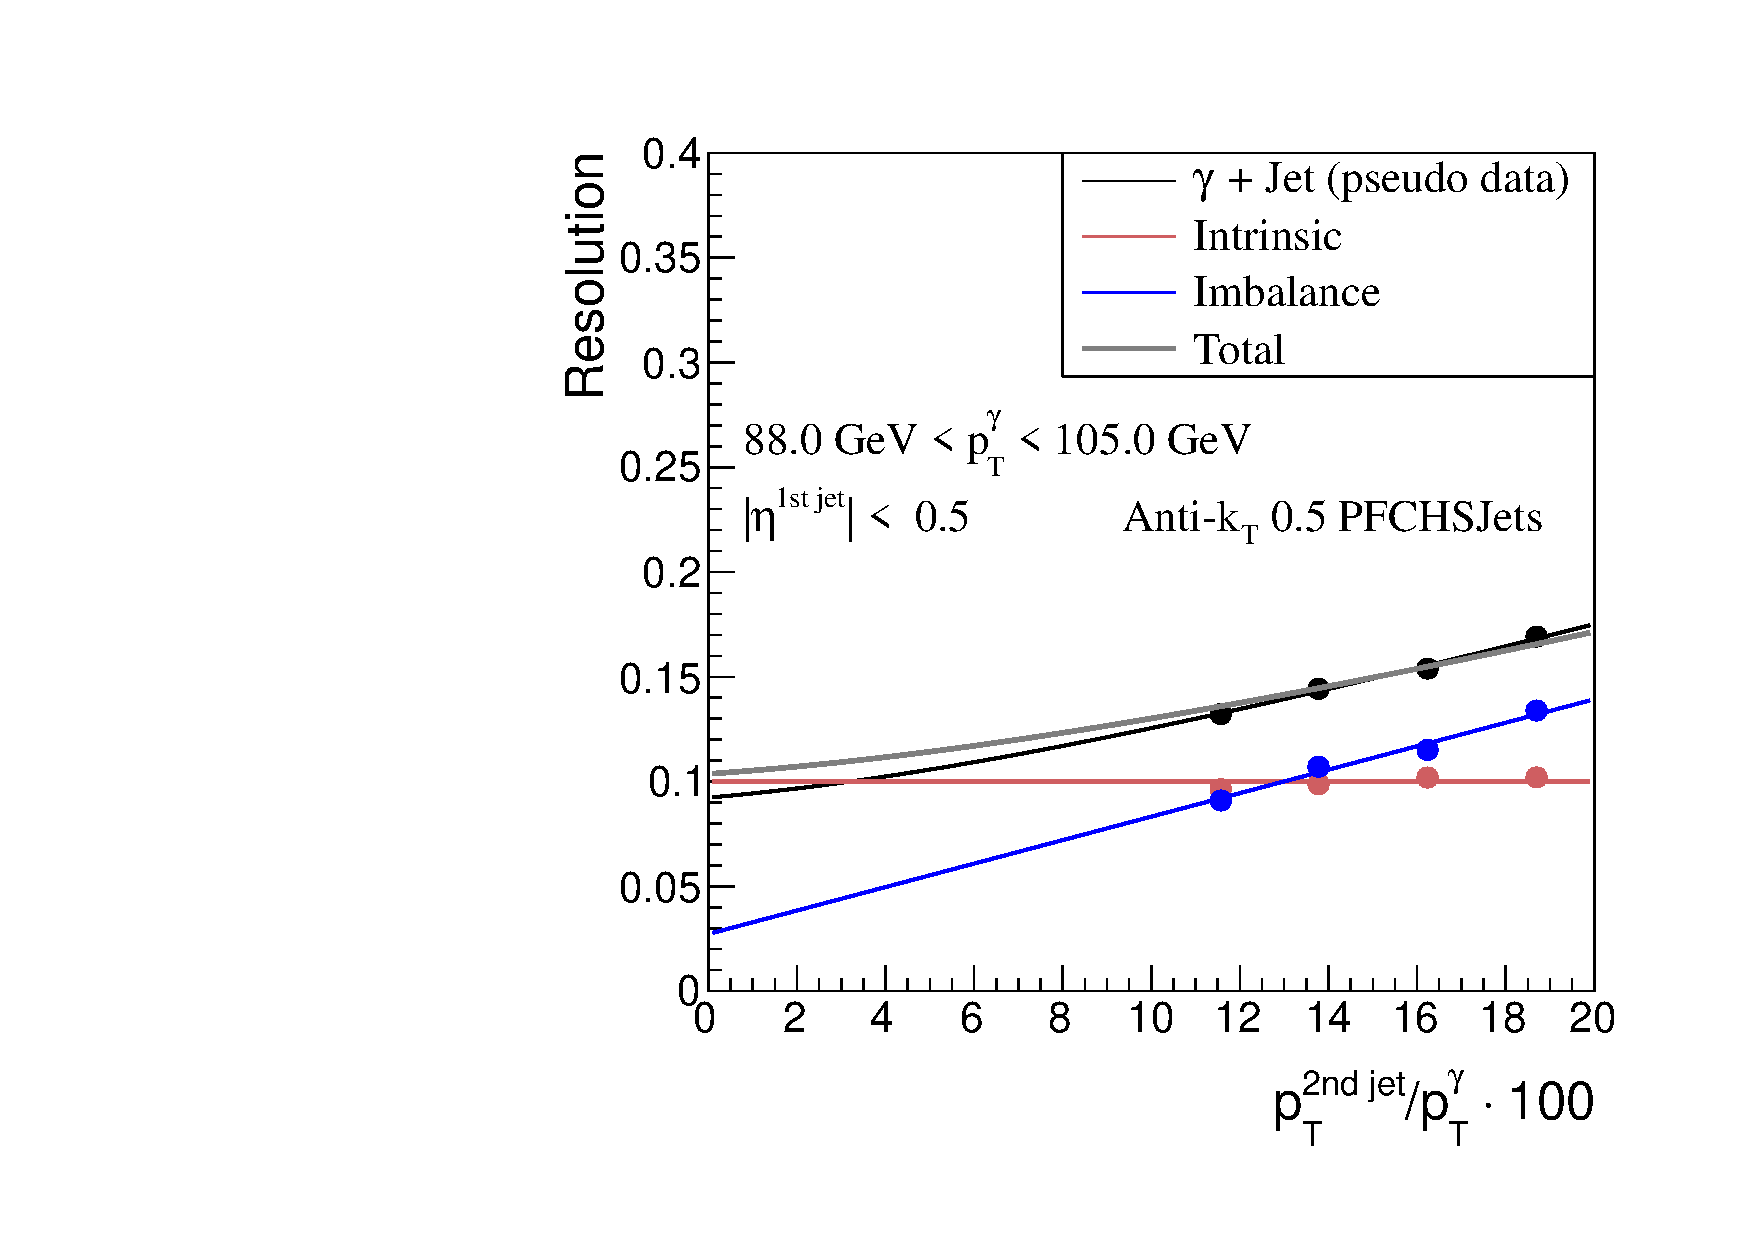
\includegraphics[width=0.49\textwidth]{figures/resolution/methodology/JER_for_1_eta_bin_4_pTGamma_bin_all_contributions_PFCHS_RMS99_mc.pdf} 
    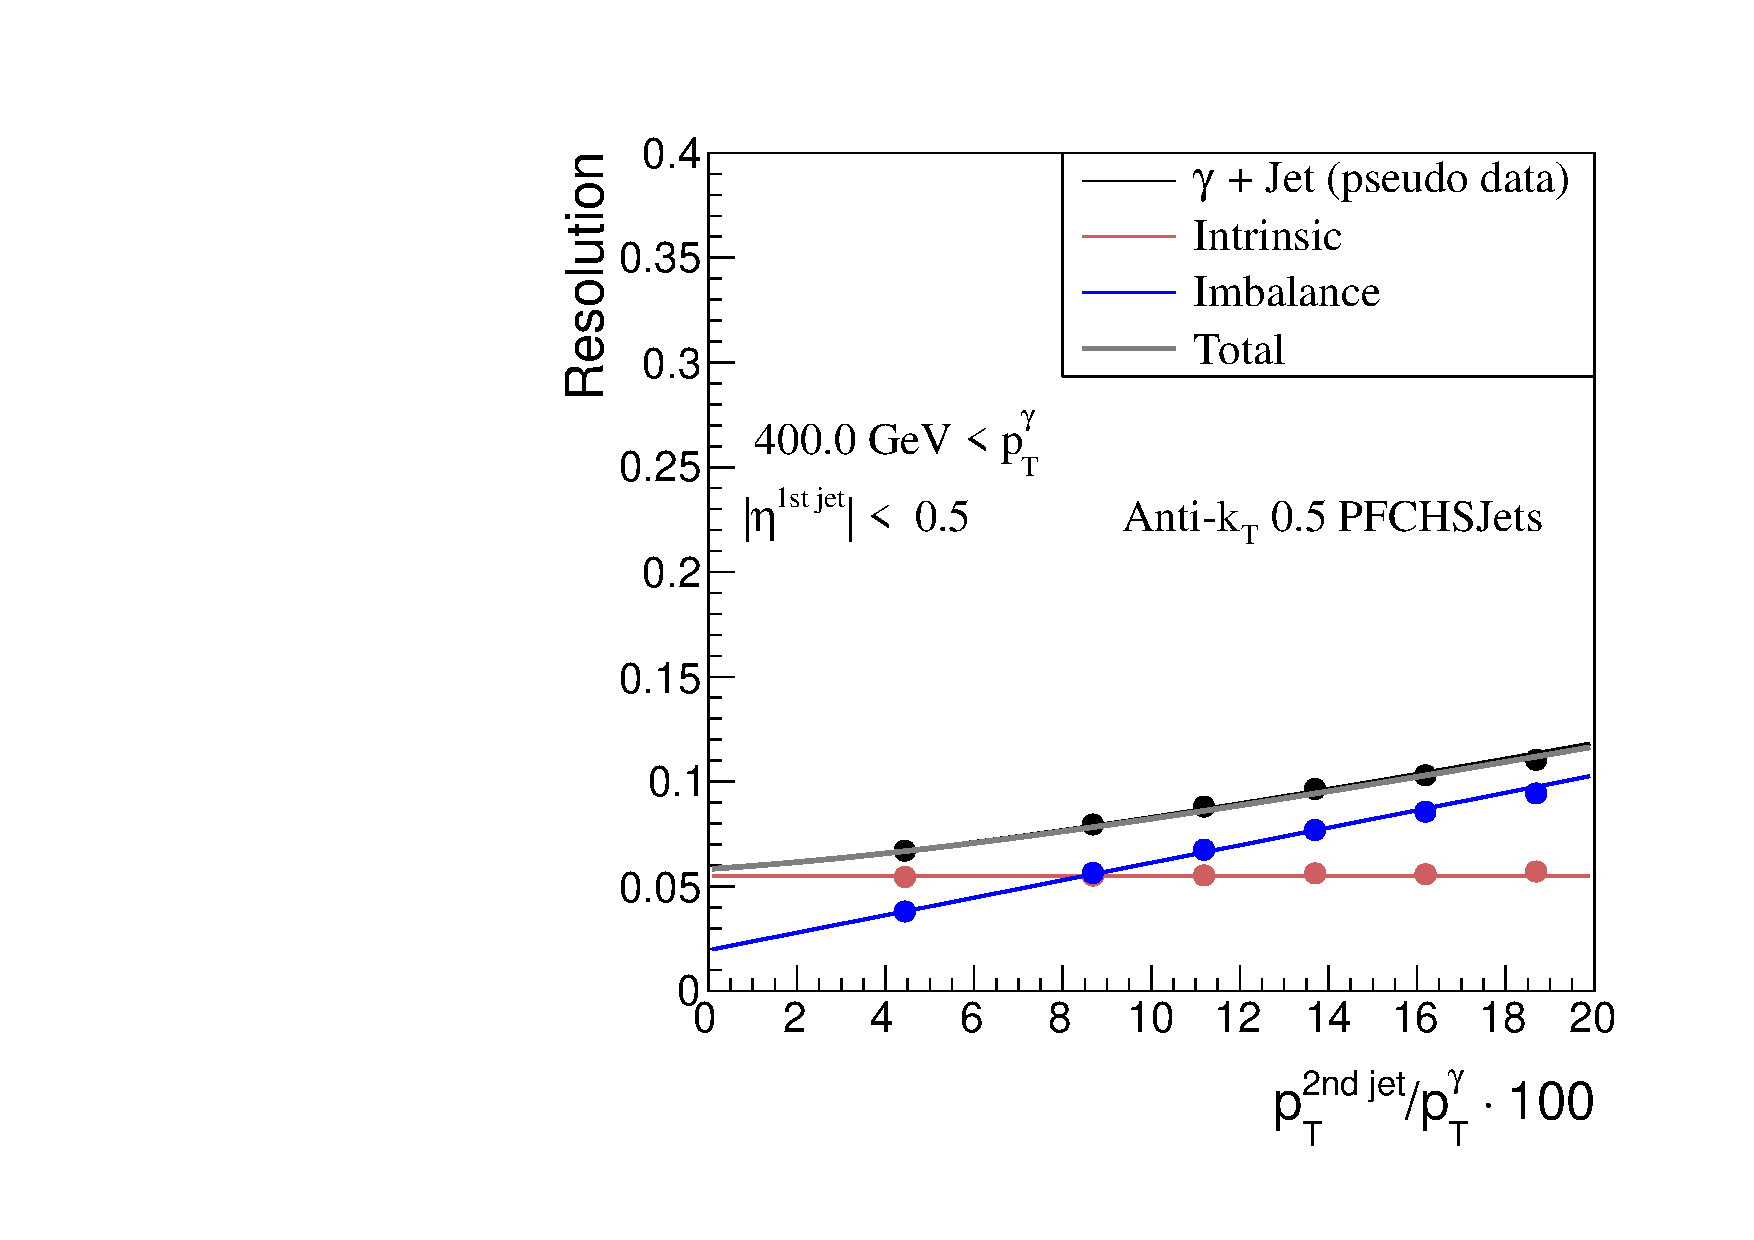
\includegraphics[width=0.49\textwidth]{figures/resolution/methodology/JER_for_1_eta_bin_12_pTGamma_bin_all_contributions_PFCHS_RMS99_mc.pdf} 
  \caption{The alpha dependency of the various parts of the resolution in the simulated events for (left) $83 \gev < \pt^{\gamma} < 99 \gev $ and (right) $400 \gev < \pt^{\gamma}$. The total resolution (Gray line) is the addition in quadrature of the imbalance (blue line) and the intrinsic (red line) 
  fit functions. It can 
  be compared to the measured pseudo data (black line).}  
 \label{fig:AlphaDependenceOfResolutions}
\end{figure}
The measured intrinsic resolution and imbalance for various $\alpha$ values are fitted with functions \eqref{eq:intrinsic} and \eqref{eq:imbalance}, respectively.
The measured total resolution (black dots) is fitted with function \eqref{eq:total}. Here, only $c$ and $m$ are free parameters, 
whereas $q$ is fixed to the value obtained from the imbalance fit. 
All contributions are well described by their fit functions. 
The gray line is the total resolution with the analytic expression of function \eqref{eq:total} with the parameters set to the fit values of the intrinsic and the imbalance fit. 

It is apparent that the imbalance is not zero for $\alpha=0$. This has two reasons.
First and most important, only the photon and the parton are balanced in the transverse plane, 
not necessarily the particles which are measured in the detector after hadronization. 
Because of the necessity of a jet reconstruction algorithm (Anti-k$_{\text{t}}$ in this analysis) with finite cone size, 
it can happen that not all particles which belong to a jet are covered by 
that algorithm (out-of-cone showering) and the photon and the particle-level jet are not balanced anymore (even for $\alpha = 0$). Second, also the photon \pt can 
be wrongly measured and spoil the residual imbalance $q$. 

These two effects lead to a small discrepancy between the measured resolution (black) and the intrinsic (red) also for zero second jet energy. 
To correct for this effect,  $q$ is fixed to the value obtained 
from fitting the imbalance part of the resolution (Eq.~\eqref{eq:imbalance}) and then only the fit parameter  $c$ is taken as the relevant resolution from the fit.
Also for measured data, $q$ is fixed to the value obtained from simulation. 
Figure~\ref{fig:ImbalanceOfPtgamma} shows the residual imbalance for two exemplary $\eta^{\text{1st jet}}$ bins. 
It is almost stable and around 2\% over the whole photon \pt range.
\begin{figure}[!b]
  \centering
    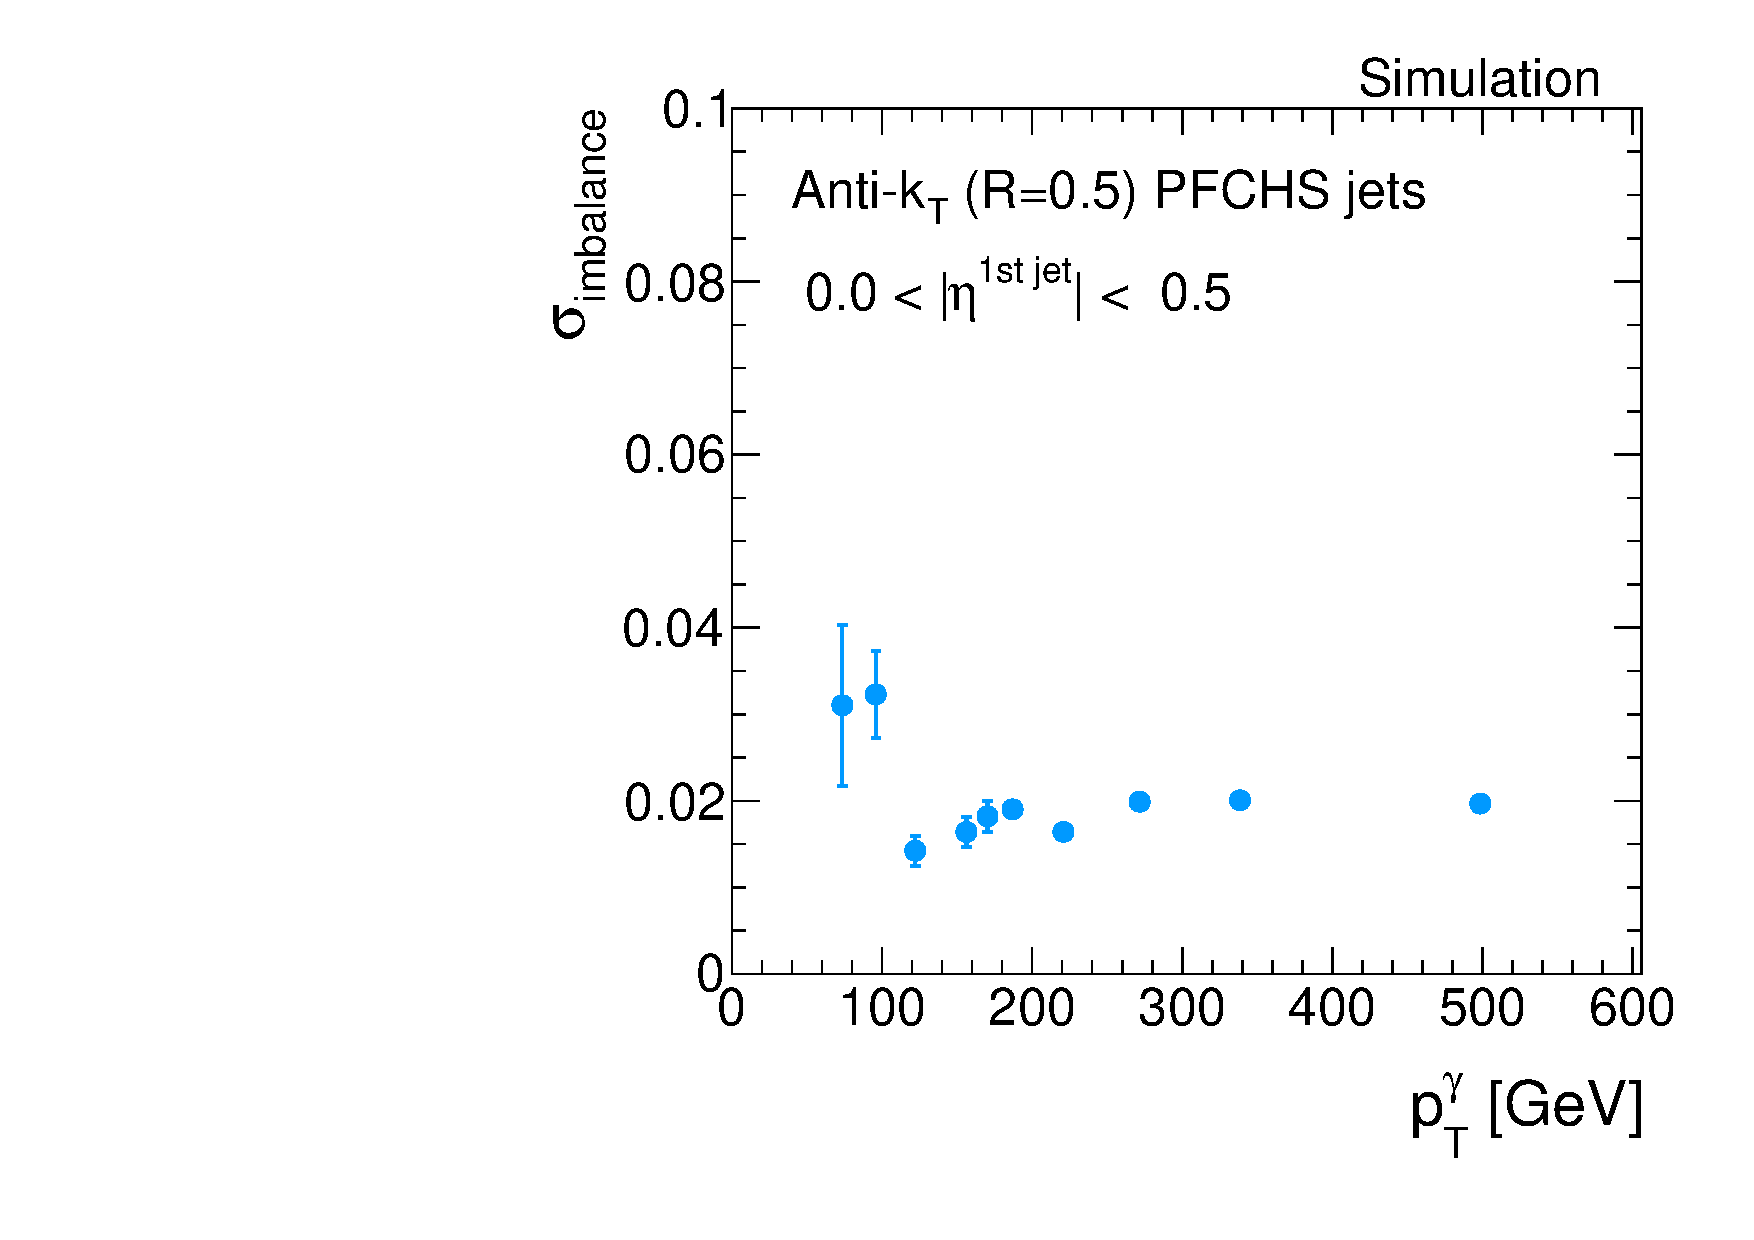
\includegraphics[width=0.49\textwidth]{figures/resolution/methodology/Imbalance_for_1_eta_bin_PFCHS_mc_RMS99.pdf}
    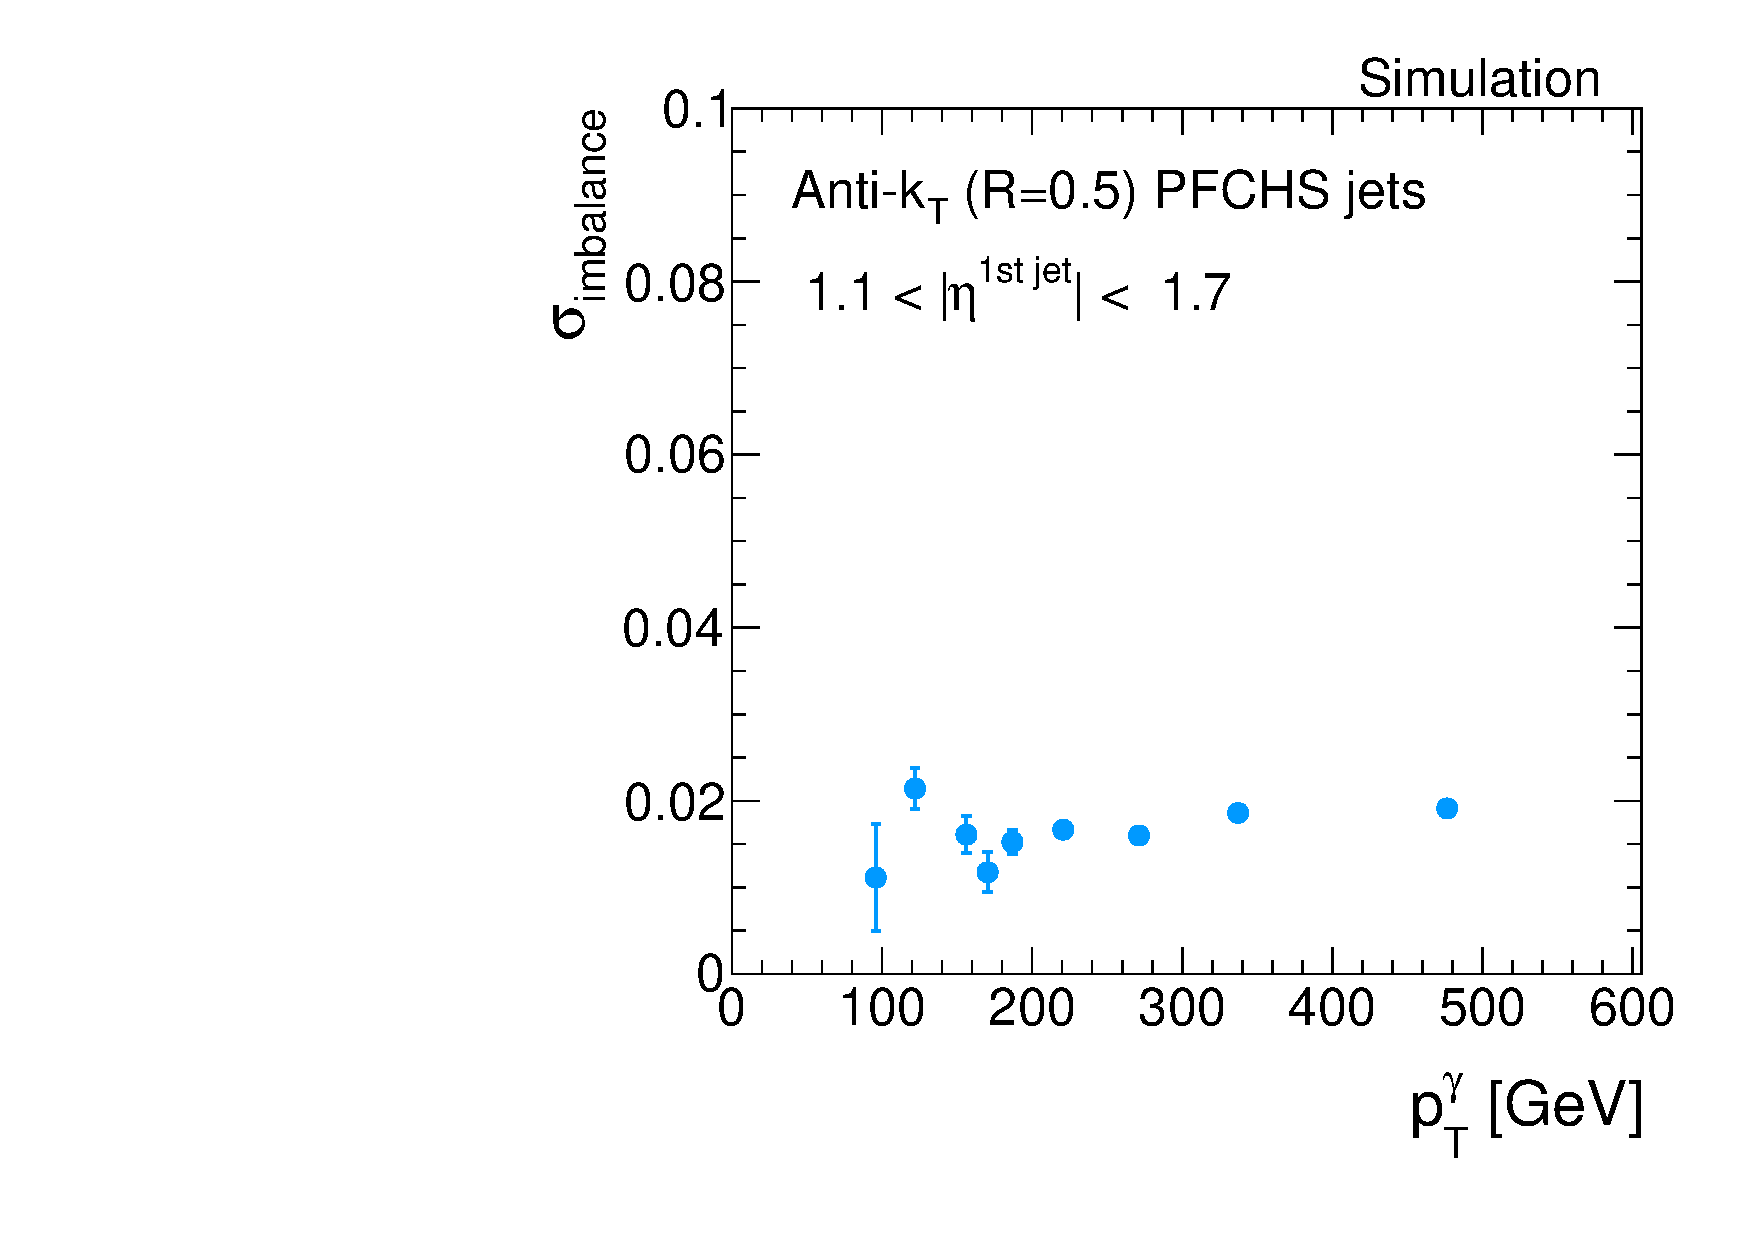
\includegraphics[width=0.49\textwidth]{figures/resolution/methodology/Imbalance_for_3_eta_bin_PFCHS_mc_RMS99.pdf}
  \caption{Imbalance for $|\eta^{\text{1st jet}}| < 0.5$ (left) and $1.1<|\eta^{\text{1st jet}}| < 1.7$ (right) in simulation.}  
  \label{fig:ImbalanceOfPtgamma}
\end{figure}

In Fig.~\ref{fig:ResolutionOfPtgamma}, the fitted intrinsic resolution in simulation is shown in the different photon \pt bins for two different $\eta^{\text{1st jet}}$ regions.
The resolution improves for increasing photon \pt. 
\begin{figure}[tbp]
  \centering
    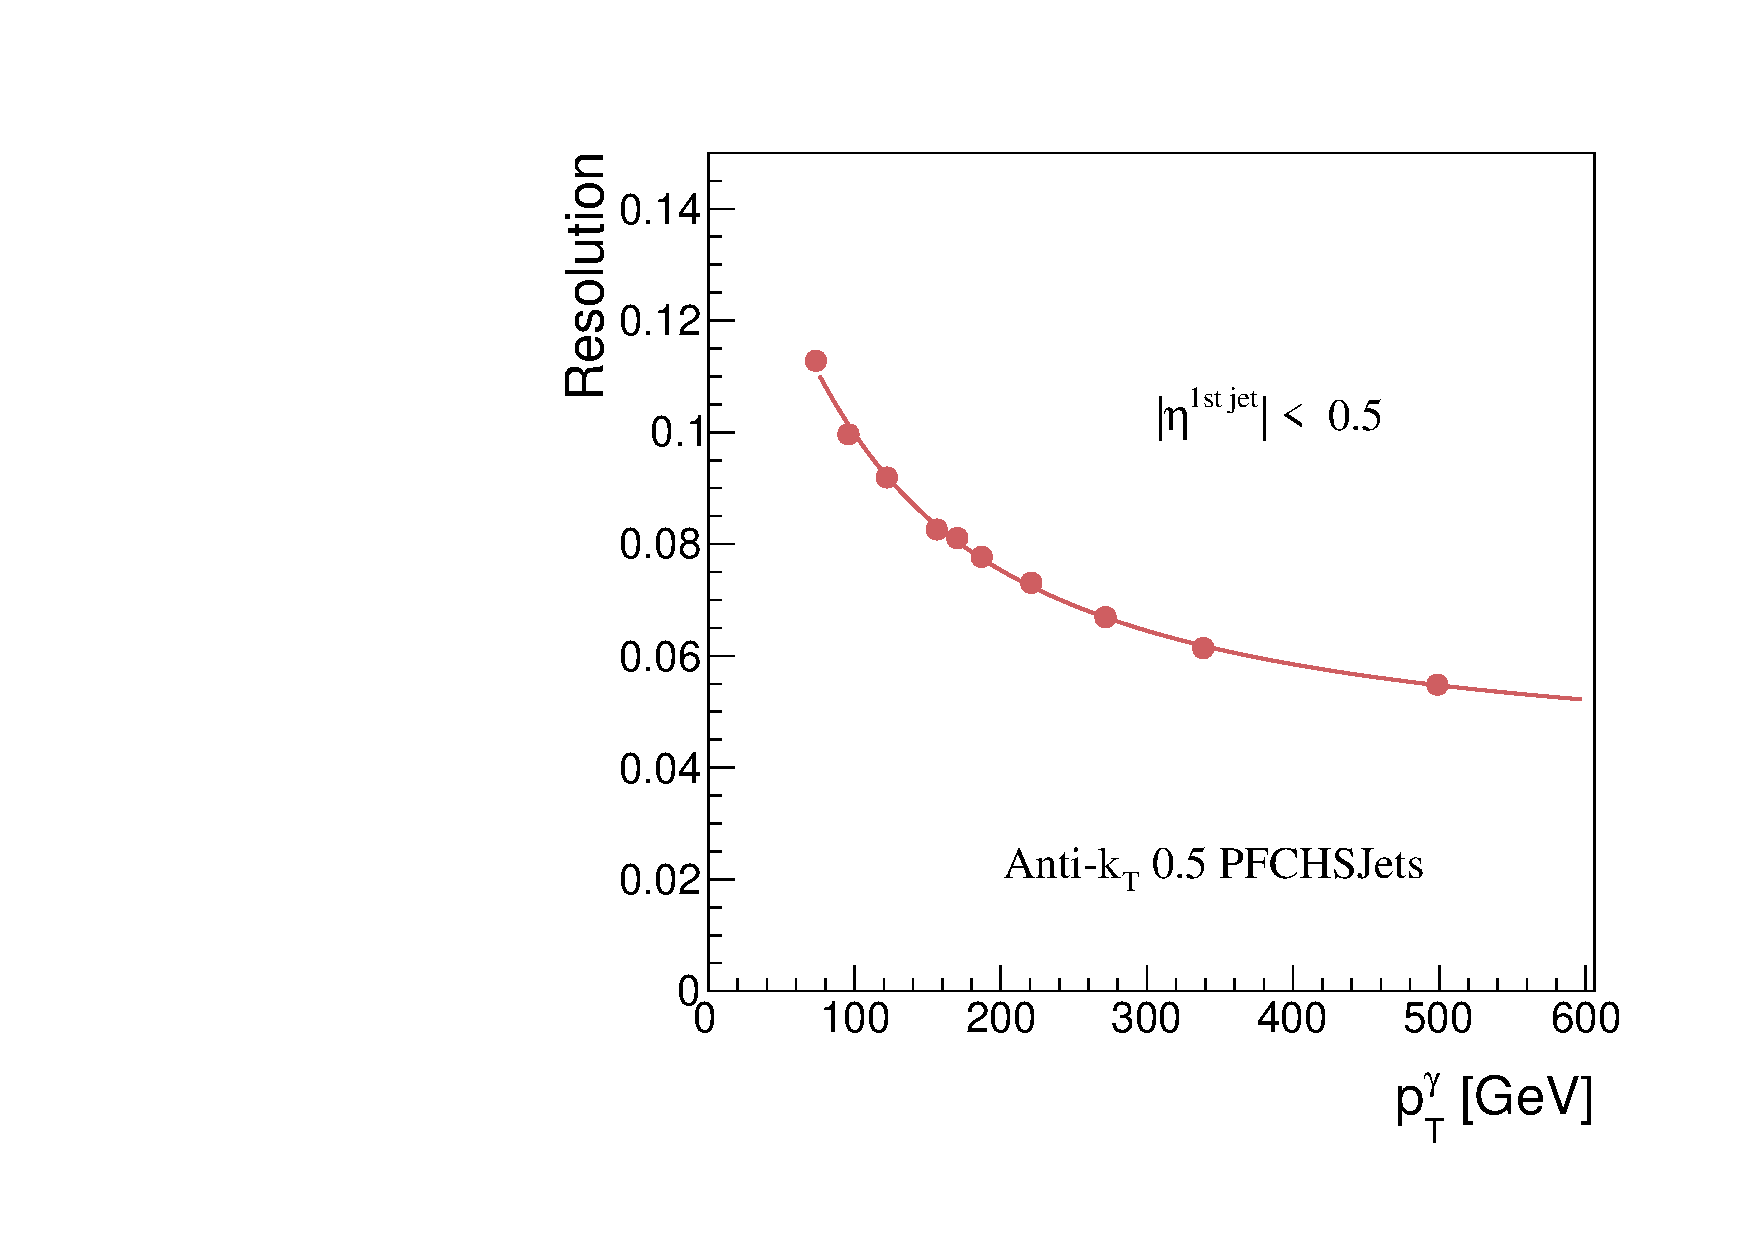
\includegraphics[width=0.49\textwidth]{figures/resolution/methodology/Resolution_for_1_eta_bin_PFCHS_mc_RMS99.pdf}
    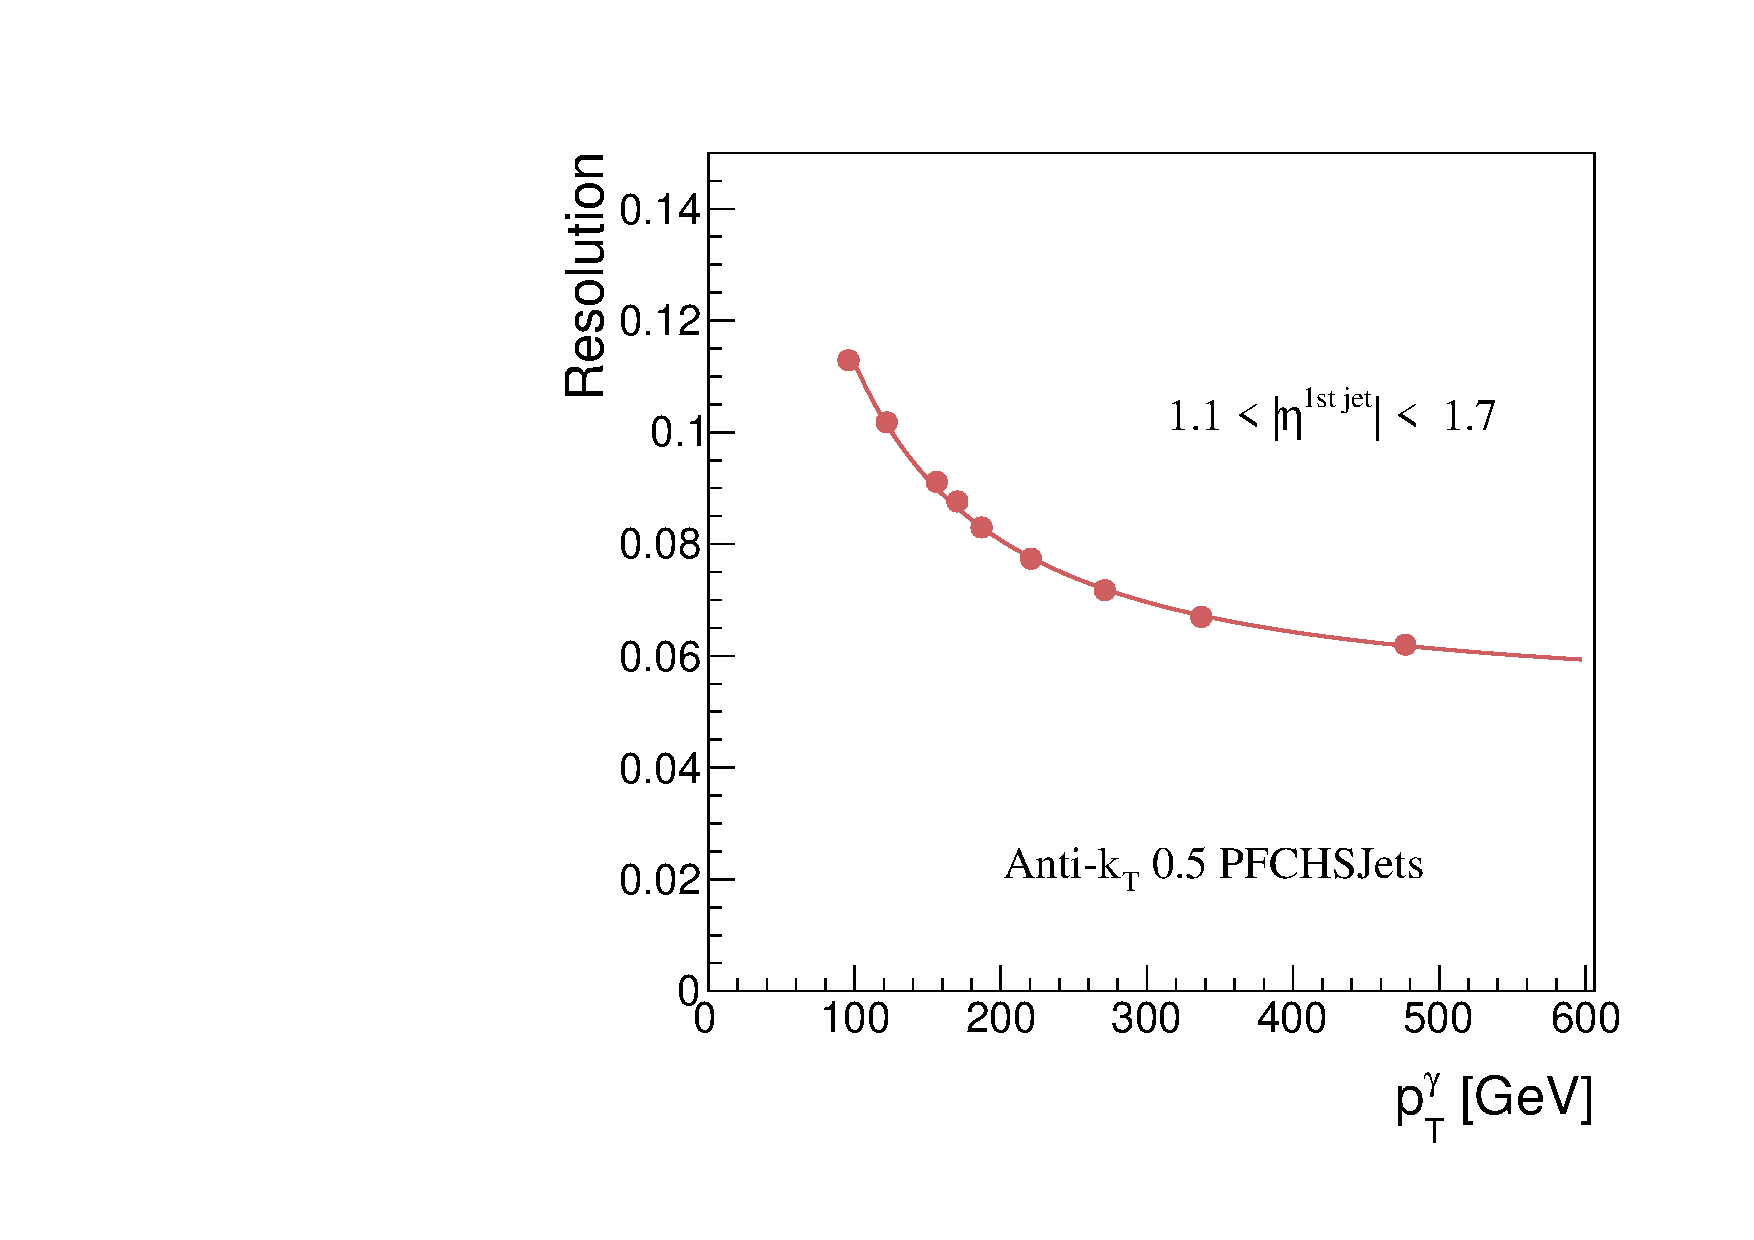
\includegraphics[width=0.49\textwidth]{figures/resolution/methodology/Resolution_for_3_eta_bin_PFCHS_mc_RMS99.pdf}
  \caption{Intrinsic resolution for $|\eta^{\text{1st jet}}| < 0.5$ (left) and $1.1<|\eta^{\text{1st jet}}| < 1.7$ (right) in simulation.}  
  \label{fig:ResolutionOfPtgamma}
\end{figure}
For the $|\eta^{\text{1st jet}}|<0.5$ region, the resolution is approximately 10\% for $\pt^{\gamma} \approx 100\gev$ and decreases to values around 6\% for  
$\pt^{\gamma} \approx 500\gev$.
The increasing statistical uncertainties for low photon \pt arise through the requirement of a maximal $\alpha$ and a minimal \pt of the second jet. 
This reduces the numbers of events in the low photon \pt bins. 
For events with $\ptgamma \lesssim 50\gev$, it is not possible at all to fulfill both requirements at the same time.

The extrapolated intrinsic resolutions for the various photon \pt are fitted with the following function
\begin{equation}
\label{eq:PFresolution}
\jer = \sqrt{\text{sgn(N)} \cdot \frac{\text{N}}{\pt}  + \text{S}^2 \cdot \pt^{\text{M}-1} +  \text{C}^2 }
\end{equation}
which was introduced for particle flow jets in \cite{bib:CMS:JERCPaper_2011}. 
It is an extended fit function compared to the usual calorimeter resolution parametrization to account for higher resolution due to tracking information. 

\section{Validation of the method}
The method is validated with simulated events. 
The bias  is shown in Fig.~\ref{fig:MCClosure} for the barrel region. 
\begin{figure}[t]
  \centering
    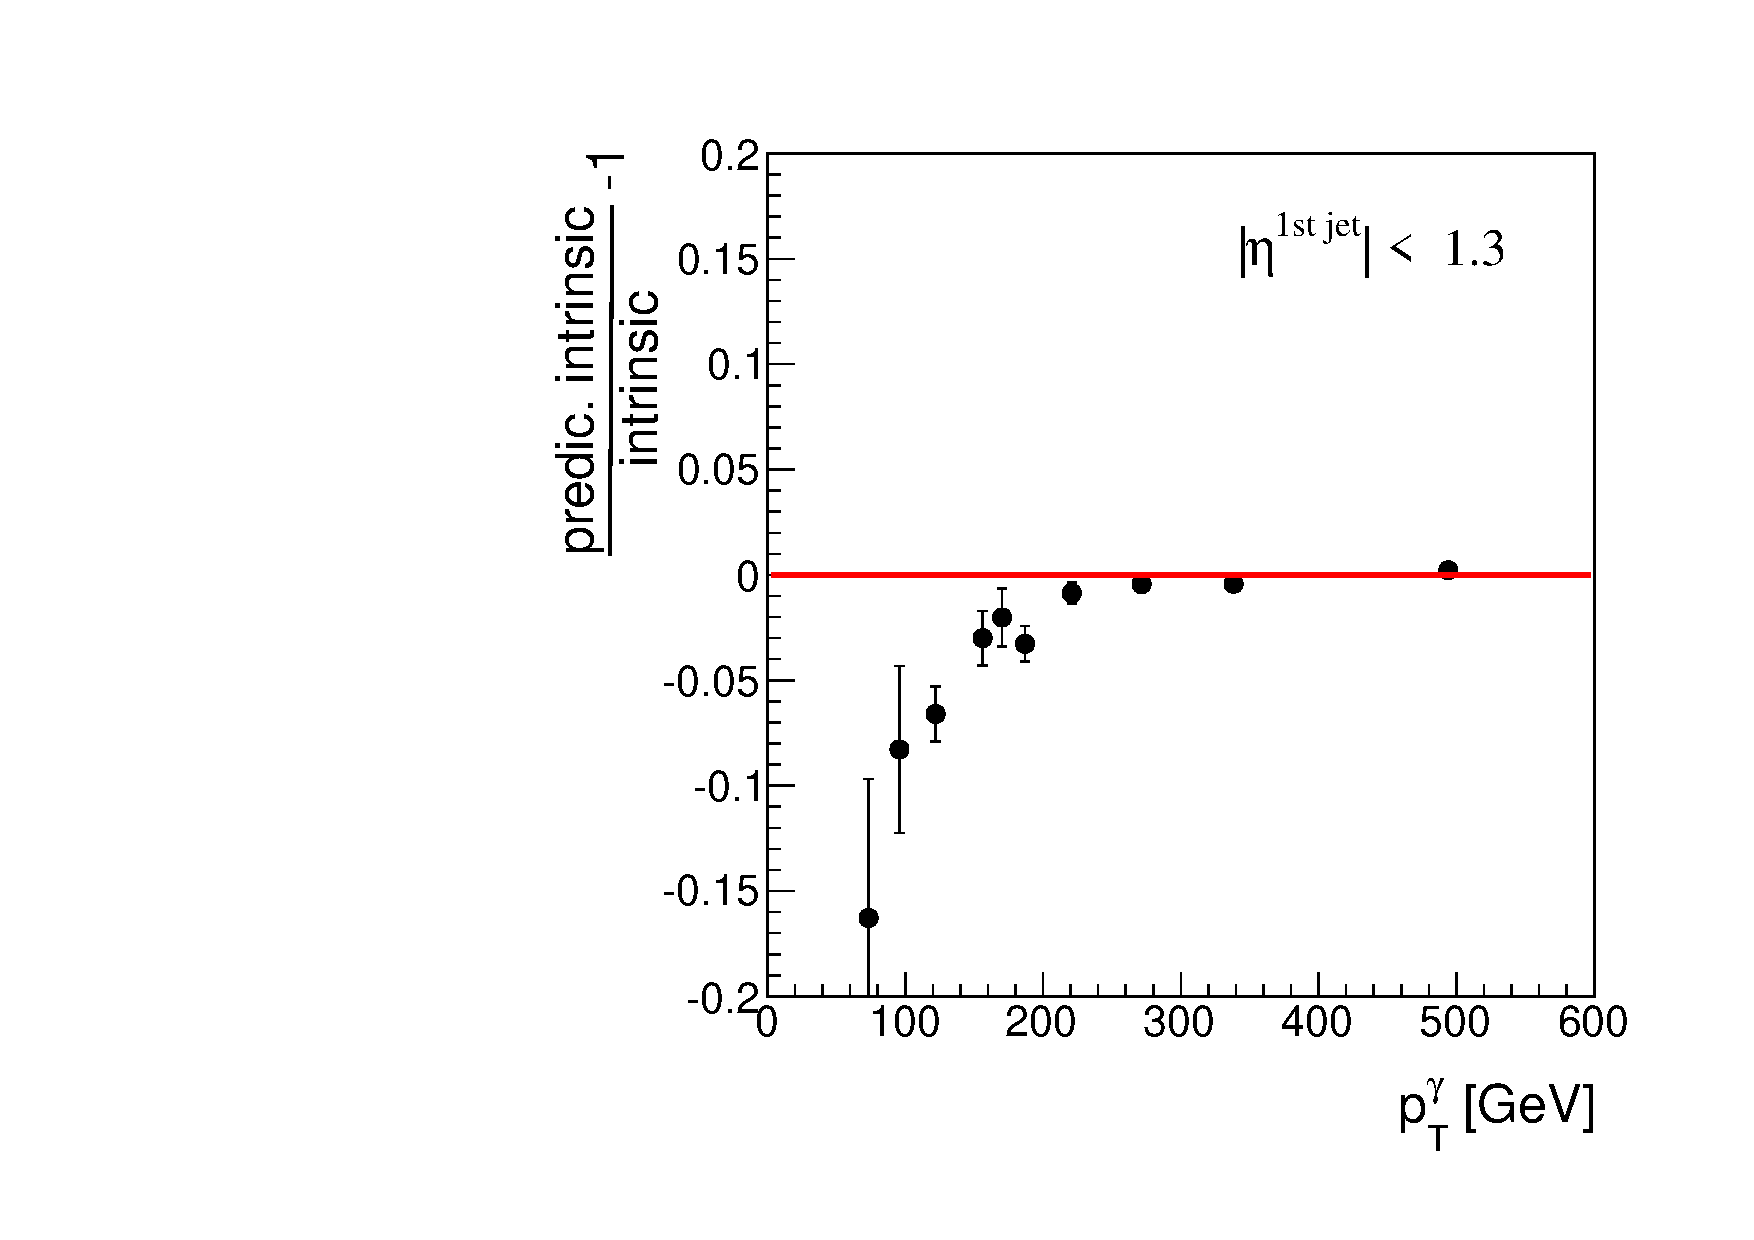
\includegraphics[width=0.49\textwidth]{figures/resolution/methodology/MCClosure_for_1_eta_bin_RMS99_barrel_0p2range.pdf}
  \caption{Consistency check of the method: Comparison between the predicted intrinsic resolution evaluated with Eq.~\eqref{eq:total} and the intrinsic resolution from Eq.~\eqref{eq:intrinsic} in simulation.}  
  \label{fig:MCClosure}
\end{figure}
It is evaluated as the ratio of the predicted intrinsic resolution by fitting Eq.~\eqref{eq:total} with $q$ fixed to the value obtained by Eq.~\eqref{eq:imbalance} over the intrinsic resolution directly obtained from the intrinsic response distribution \ptrecojet/\ptgenjet.
The result is in good agreement with the expectation to better than 5\% above 100\gev and better than 1\% above 200\gev.
Only for small \pt, larger deviations are observed, which are systematically lower than zero (up to 15\%).

%The residual bias of the method for small $\pt^{\gamma}$ is originating from the $\alpha$ definition 
%and the decreasing dependence of the resolution on $\pt^{\gamma}$ shown in Figs. \ref{fig:ResolutionOfPtgamma} (a) and (b):\\
%In every $\alpha$ and photon \pt bin, there is a range of various jet \pt.
%Especially for small photon \pt, this leads to differences in the intrinsic resolutions within one $\pt^\gamma$ bin because of the strong $\pt^{\gamma}$ dependence of the resolution.
%Because of the $\alpha$ definition (\mbox{Eq.~\eqref{eq:alphaDef}}) jets with high \pt (and thus better resolution)
%accumulate in the low $\alpha$ bins, whereas jets with low \pt fall in the high $\alpha$ bins. 
%This behavior can be seen in the intrinsic resolution 
%in \mbox{Fig. \ref{fig:AlphaDependenceOfResolutions} \ref{fig:small}}, where a small increase of the resolution to high $\alpha$ can be seen. 
%By fitting a horizontal line to the intrinsic resolution, this effect is averaged out. 
%But the measured resolution with an additional free parameter 
%can adopt this increase and result, therefore, in a y-intercept which is too small. 
%For high photon \pt bins, this effect is less pronounced, as the slope of JER($\pt^{\gamma}$) flattens out.

The residual bias of the method for small \ptgamma is stemming from two effects: 
First, the binning in \ptgamma and the momentum balance between the photon and the first two jets lead to a dependency of the first jet \pt on the second jet \pt and therefore alpha: 
For a fixed \ptgamma, 
%the greater the second jet pt, the smaller the first jet \pt for events where the second jet is in the leading jet hemisphere 
the \pt of the first jet gets smaller for larger $\pt^{\text{2nd jet}}$ for events where the second jet is in the leading jet hemisphere (see Fig.~\ref{fig:sketch}), leading to a dependency of $\pt^{\text{1st jet}} \propto -\pt^{\text{2nd jet}}$.
This effect is directly opposite for events with a second jet in the photon hemisphere. 
In these events, the first jet \pt gets larger for larger $\pt^{\text{2nd jet}}$ and thus $\pt^{\text{1st jet}} \propto \pt^{\text{2nd jet}}$ for fixed \ptgamma. 
As the resolution of the jet improves with higher jet \pt (see Fig.~\ref{fig:ResolutionOfPtgamma}), 
a dependency of the leading jet \pt on the second jet \pt directly leads to a dependency of the intrinsic resolution on the second jet \pt. 
In principle, as the effect is opposite for events in the different hemispheres, it should cancel out, when taking the weighted mean of the two hemisphere resolutions. 
But as the topology of a second jet in the leading jet hemisphere is much more frequent, a residual upwards trend in the intrinsic resolution vs. $\alpha$ is conserved. 

The second source of the residual bias arises from the alpha definition $\alpha = \frac{\pt^{\text{2nd jet}}}{\pt^{\gamma}}$. 
Because of the inclusion of $\pt^{\gamma}$ in $\alpha$ with $\alpha \propto \frac{1}{\pt^{\gamma}}$, 
the high photon \pt events accumulate in the low alpha regions. 
As the selected events are almost balanced, a high $\pt^{\gamma}$ is associated with a high jet \pt, thus also the high jet \pt events accumulate in the low alpha bins, 
leading to  an upward trend in the intrinsic resolution. This behavior can be seen in the intrinsic resolution 
in Fig.~\ref{fig:AlphaDependenceOfResolutions}, where a small increase of the resolution to high $\alpha$ can be seen. 
By fitting a horizontal line to the intrinsic resolution, this effect is averaged out. 
But the measured resolution with an additional free parameter 
can adopt this increase and result, therefore, in a y-intercept which is too small. 
For high photon \pt bins, this effect is less pronounced, as the slope of JER($\pt^{\gamma}$) (see Fig.~\ref{fig:AlphaDependenceOfResolutions}) flattens out.

However, this is not of concern here, because the results of the measurement will be presented as resolution scaling factors, defined as the resolution measured in data divided by
the resolution measured in Monte Carlo simulation (MC) $\jerintr^{\text{data}}$/$\jerintr^{\text{MC}}$. 
Hence, a possible bias in the separate resolution measurements for data and simulation cancels out. 

As the data to simulation ratio was empirically found to be independent of \ptgamma, it can be fitted with a constant.
Thus resulting in only one scaling factor for every $\eta^{\text{1st jet}}$ region.


To prove the hypothesis of the cancellation of the bias, the data set with simulated events was additionally smeared with some input values for various $\eta^{\text{1st jet}}$ bins. 
After measuring the resolution of the smeared and non-smeared data set, the relative difference between the two data sets ($\jerintr^{\text{smeared MC}}/\jerintr^{\text{non-smeared MC}}$) is fitted with a constant over the photon \pt range. 
The resulting numbers (one for each $\eta^{\text{1st jet}}$ bin) are then compared to the input factors. 

In Fig.~\ref{fig:MCClosureRatio}, a comparison of the input and output values is shown. 
The resolution is hereby defined in three different ways: The standard deviations of the 99\% and 95\% truncated response distribution and as the width of a Gaussian\footnote{The Gaussian width is defined as the standard deviation of the 2$\sigma$ interval (core region) around the mean, where the determination of $\mu$ and $\sigma$ were approximated with an iterative procedure.}.
\begin{figure}[tbp]
  \centering
    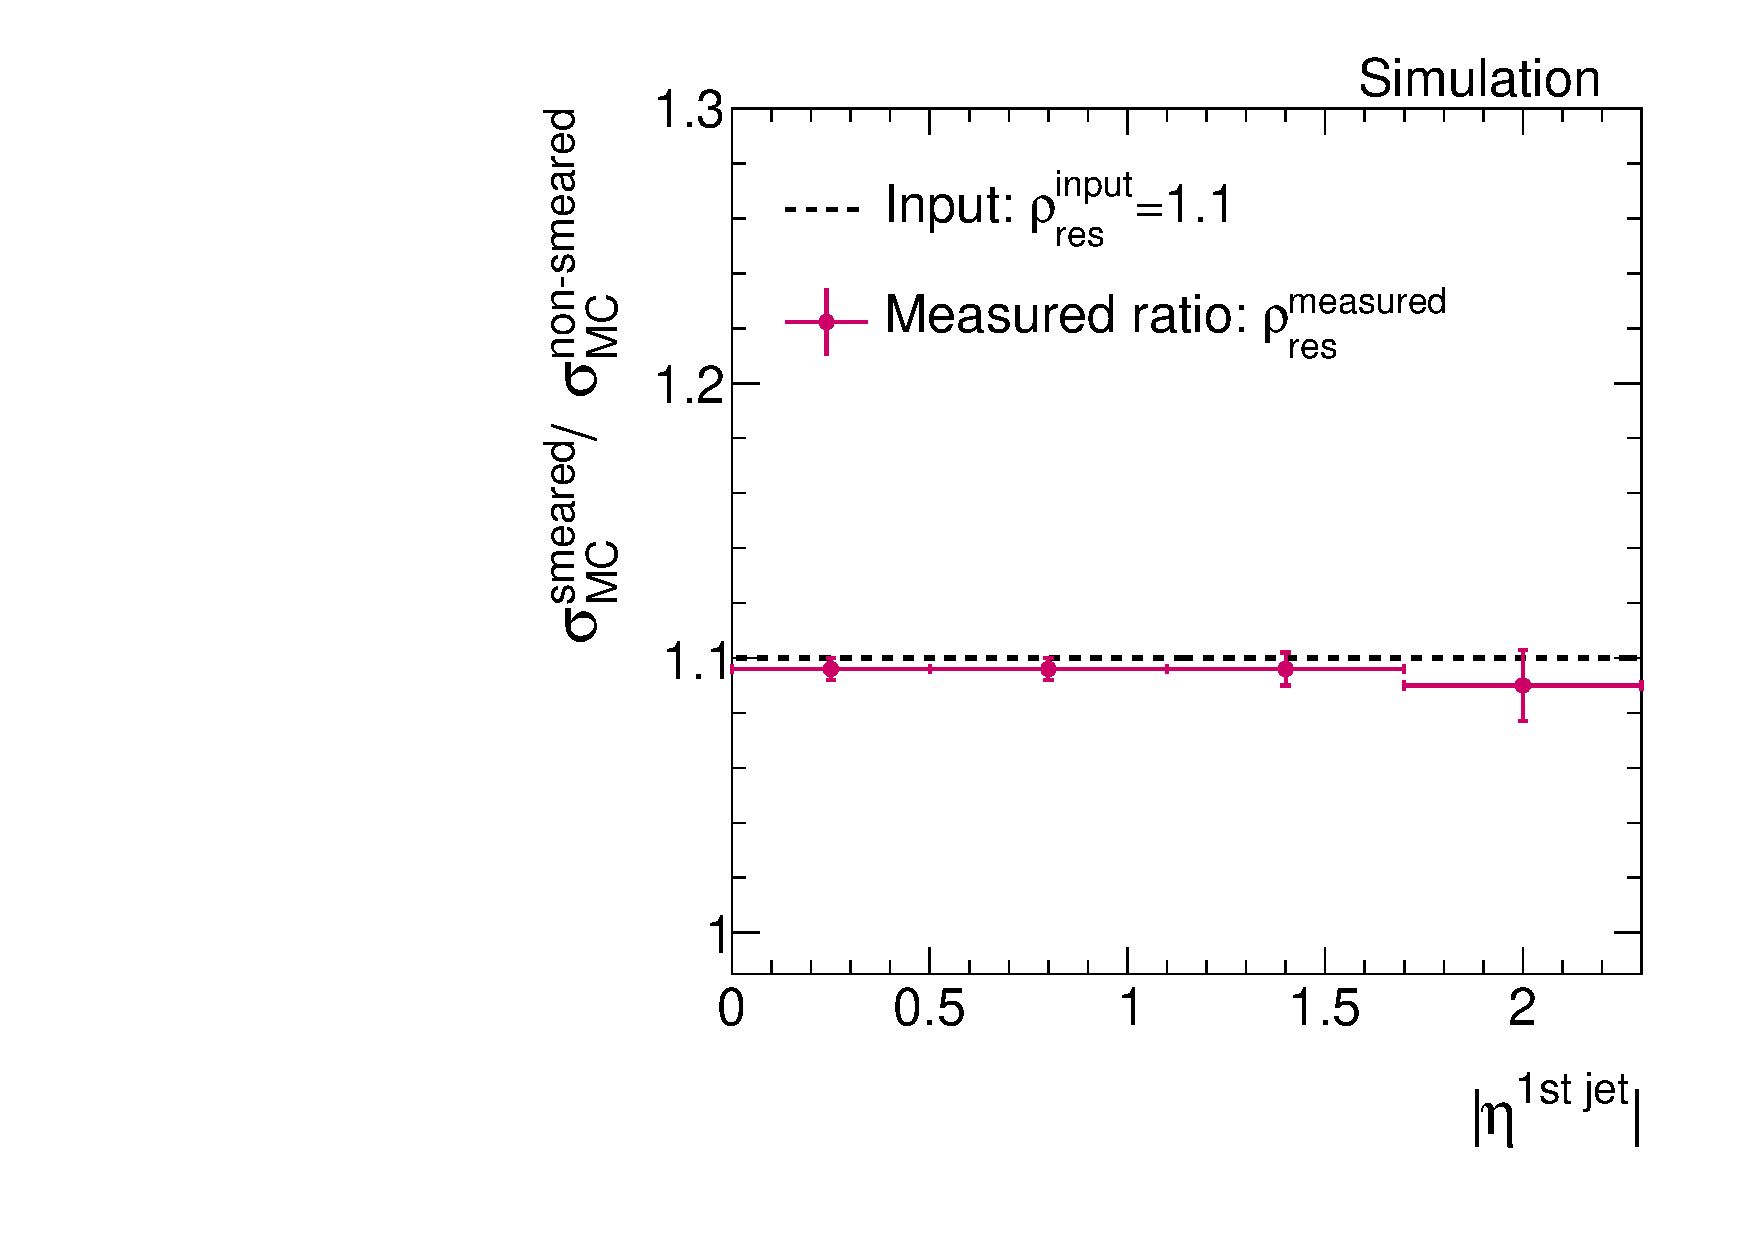
\includegraphics[width=0.49\textwidth]{figures/resolution/methodology/MCClosureRatio.pdf}
     \caption{Comparison of the resolution ratios $\jerintr^{\text{smeared MC}}/\jerintr^{\text{non-smeared MC}}$ measured in simulated events with the input smearing factors 1.05, 1.07, 1.09 and 1.11 (black dots) 
              for the various $\eta^{\text{1st jet}}$ bins, respectively. 
              Shown are the results for a Gaussian fit of the response distribution (blue triangles), a standard deviation of the 99\% (red squares) and the 95\% truncated response (green dots).}
  \label{fig:MCClosureRatio}
\end{figure}

In all cases, the measurement reproduces the input factors.
However, in this analysis the 99\% truncated response will be used to be consistent with the defintion from \cite{bib:CMS-AN-2010-076}.

In the following section, the systematic uncertainties will be discussed. 
Afterward, results for 8\tev data will be presented.


%%%%%%%%%%%%%%%%%%%%%%%%%%%%%%%%%%%%%%%%%%%%%%%%%%%%%%%%%%%%%%%%%%%%%%%%%%%%%%%%%%%%%%%%%%%%%%%%%%%%%%%%%%%%%%%%%%%%%%%%%%%%%%%%%%%%%%%%%%%%%%%%%%%%%%%%%%%%%%%%%%%%%%%%%%%%%%%%%%%%%%%%%%%%%%%%%%%%%%%%%%%%%%%%%%%%%%%%%%%%%%%%%%%%%%%%%%%

%%%%%%%%%%%%%%%%%%%%%%%%%%%%%%%%%%%%%%%%%%%%%%%%%%%%%%%%%%%%%%%%%%%%%%%%%%%%%%%%%%%%%%%%%%%%%%%%%%%%%%%%%%%%%%%%%%%%%%%%%%%%%%%%%%%%%%%%%%%%%%%%%%%%%%%%%%%%%%%%%%%%%%%%%%%%%%%%%%%%%%%%%%%%%%%%%%%%%%%%%%%%%%%%%%%%%%%%%%%%%%%%%%%%%%%%%%%
%%%%%%%%%%%%%%%%%%%%%%%%%%%%%%%%%%%%%%%%%%%%%%%%%%%%%%%%%%%%%%%%%%%%%%%%%%%%%%%%%%%%%%%%%%%%%%%%%%%%%%%%%%%%%%%%%%%%%%%%%%%%%%%%%%%%%%%%%%%%%%%%%%%%%%%%%%%%%%%%%%%%%%%%%%%%%%%%%%%%%%%%%%%%%%%%%%%%%%%%%%%%%%%%%%%%%%%%%%%%%%%%%%%%%%%%%%%
\FloatBarrier
\chapter{Systematic uncertainties}

Many systematic uncertainties of the jet energy resolution measurement cancel out when focusing on the data to simulation ratio $\frac{\text{JER}^{\text{data}}}{\text{JER}^{\text{MC}}}$.
In the following subsections, only uncertainties relevant for this ratio will be discussed.

For the final uncertainty, the single uncertainties are added in quadrature, 
resulting in a relative uncertainty of $2.3\%$ to $6.3\%$ for the lowest and highest $\eta$ bin, respectively. 

An overview of all systematic uncertainties can be found in \mbox{table \ref{tab:Uncertainties}}.


\begin{table}[t]
\caption{All relative systematic uncertainties on the data to simulation ratio $\frac{\text{JER}^{\text{data}}}{\text{JER}^{\text{MC}}}$ listed by sources for the different $|\eta|$ bins.}
\renewcommand{\arraystretch}{1.2}
\begin{center}
\begin{tabular}{ l| c | c | c | c |}
\multicolumn{1}{c}{} & \multicolumn{4}{c}{$|\eta^{\text{Jet}}|$}\\\hline
& \textbf{0.0 - 0.5}& \textbf{0.5 - 1.1}& \textbf{1.1 - 1.7}& \textbf{1.7 - 2.3}\\\hline
\multirow{2}{*}{\textbf{Multijet contamination}}& $+2.0 \% $ & $+2.0 \% $ & $+2.3 \% $ & $+2.5 \% $ \\
& $-2.0 \% $ & $-2.0 \% $ & $-2.3 \% $ & $-2.5 \% $ \\\hline
\multirow{2}{*}{\textbf{Flavor uncertainty}}& $+0.9 \% $ & $+0.9 \% $ & $+0.8 \% $ & $+0.6 \% $ \\
& $-0.9 \% $ & $-0.9 \% $ & $-0.8 \% $ & $-0.6 \% $ \\\hline
\multirow{2}{*}{\textbf{JEC uncertainty}}& $+0.6 \% $ & $+0.6 \% $ & $+0.6 \% $ & $+0.7 \% $ \\
& $-0.5 \% $ & $-0.6 \% $ & $-0.6 \% $ & $-0.6 \% $ \\\hline
\multirow{2}{*}{\textbf{Out-of-Cone showering simulation}}& $+0.5 \% $ & $+2.8 \% $ & $+3.6 \% $ & $+5.7 \% $ \\
& $-0.5 \% $ & $-2.8 \% $ & $-3.6 \% $ & $-5.7 \% $ \\\hline
\multirow{2}{*}{\textbf{PU uncertainty}}& $+0.1 \% $ & $+0.1 \% $ & $+0.1 \% $ & $+0.2 \% $ \\
& $-0.1 \% $ & $-0.1 \% $ & $-0.2 \% $ & $-0.2 \% $ \\\hline\hline
\multirow{2}{*}{\textbf{Total}}& $+2.3 \% $ & $+3.6 \% $ & $+4.4 \% $ & $+6.3 \% $ \\
& $-2.3 \% $ & $-3.6 \% $ & $-4.4 \% $ & $-6.3 \% $ \\\hline
\end{tabular}
\end{center}
\label{tab:Uncertainties}
\end{table}

\section*{QCD-multijet contamination uncertainty}
Although the photon selection is very strict (see Section \ref{sec:eventselection}), 
due to the huge multijet cross section, a countable fraction of dijet events can survive the selection with a jet misidentified as photon.
This happens, when \eg a jet hadronizes to a $\pi^0$ that decays to two photons which is sometimes not distinguishable from the isolated photon of a $\GAMJET$ event for the detector.

In principle, those dijet events have the same topology as $\GAMJET$ events. The two leading jets are also balanced apart from initial and final state radiation. 
Therefore, the method is generally expected to hold. 
A worsening of the resolution because of background contamination is only expected due to the mismeasurement of the \pt of the jet misidentified as photon,
because only the energy of the $\pi^0$ is counted and not the full energy.
Another aspect is the different flavor composition of a QCD dijet sample. 
Due to the different production mechanism, QCD dijets are predominantly initiated by gluons 
while the leading jet in $\GAMJET$ events often stems from a light quark, cf. Fig.\ref{fig:FeynmanDiagrams}.
The number of particles after hadronization is typically larger for gluon jets, hence the single particles are less energetic and out-of-cone showering is more pronounced.
Since in this analysis the residual imbalance $q^{\prime}$ is taken from the simulation where only a $\GAMJET$ sample was analyzed, 
it is not expected to accurately describe the residual imbalance in the data sample where also dijet events occur.

To investigate the impact of multijet contamination, the following QCD dijet sample, enriched in jets with a large electromagnetic fraction, 
was added to the $\GAMJET$ sample and weighted according to the cross section:\\
\texttt{/QCD\_Pt\_*\_EMEnriched\_TuneZ2star\_8TeV\_pythia6/}\\
\texttt{Summer12\_DR53X-PU\_S10\_START53\_V7A-v1/AODSIM}.

The dijet sample has very large event weights leading to high statistical uncertainties in the measured jet energy resolution. 
Therefore, for the determination of the dijet contamination uncertainty, some selection criteria ($\alpha$<0.4 and $\Delta\Phi$>2.7) had to be relaxed, 
and a rougher binning in $\alpha$, $\pt^{\gamma}$ and $\eta^{\text{1st jet}}$ was applied in order to have enough events in every response histogram. 

The residual imbalance $q^{\prime}$ of the resolution measurement including the QCD dijet sample was fixed to the residual imbalance determined from the $\GAMJET$ only analysis to account for the possible error 
in the evaluation of the $\frac{\text{JER}^{\text{data}}}{\text{JER}^{\text{MC}}}$ ratio where data is only compared to a $\GAMJET$ sample.

In \mbox{Fig. \ref{fig:QCDuncertainty}}, the resolution measured when using both the $\GAMJET$ and the dijet sample is compared to the resolution measured only in the dijet sample.
\begin{figure}[b]
  \centering

      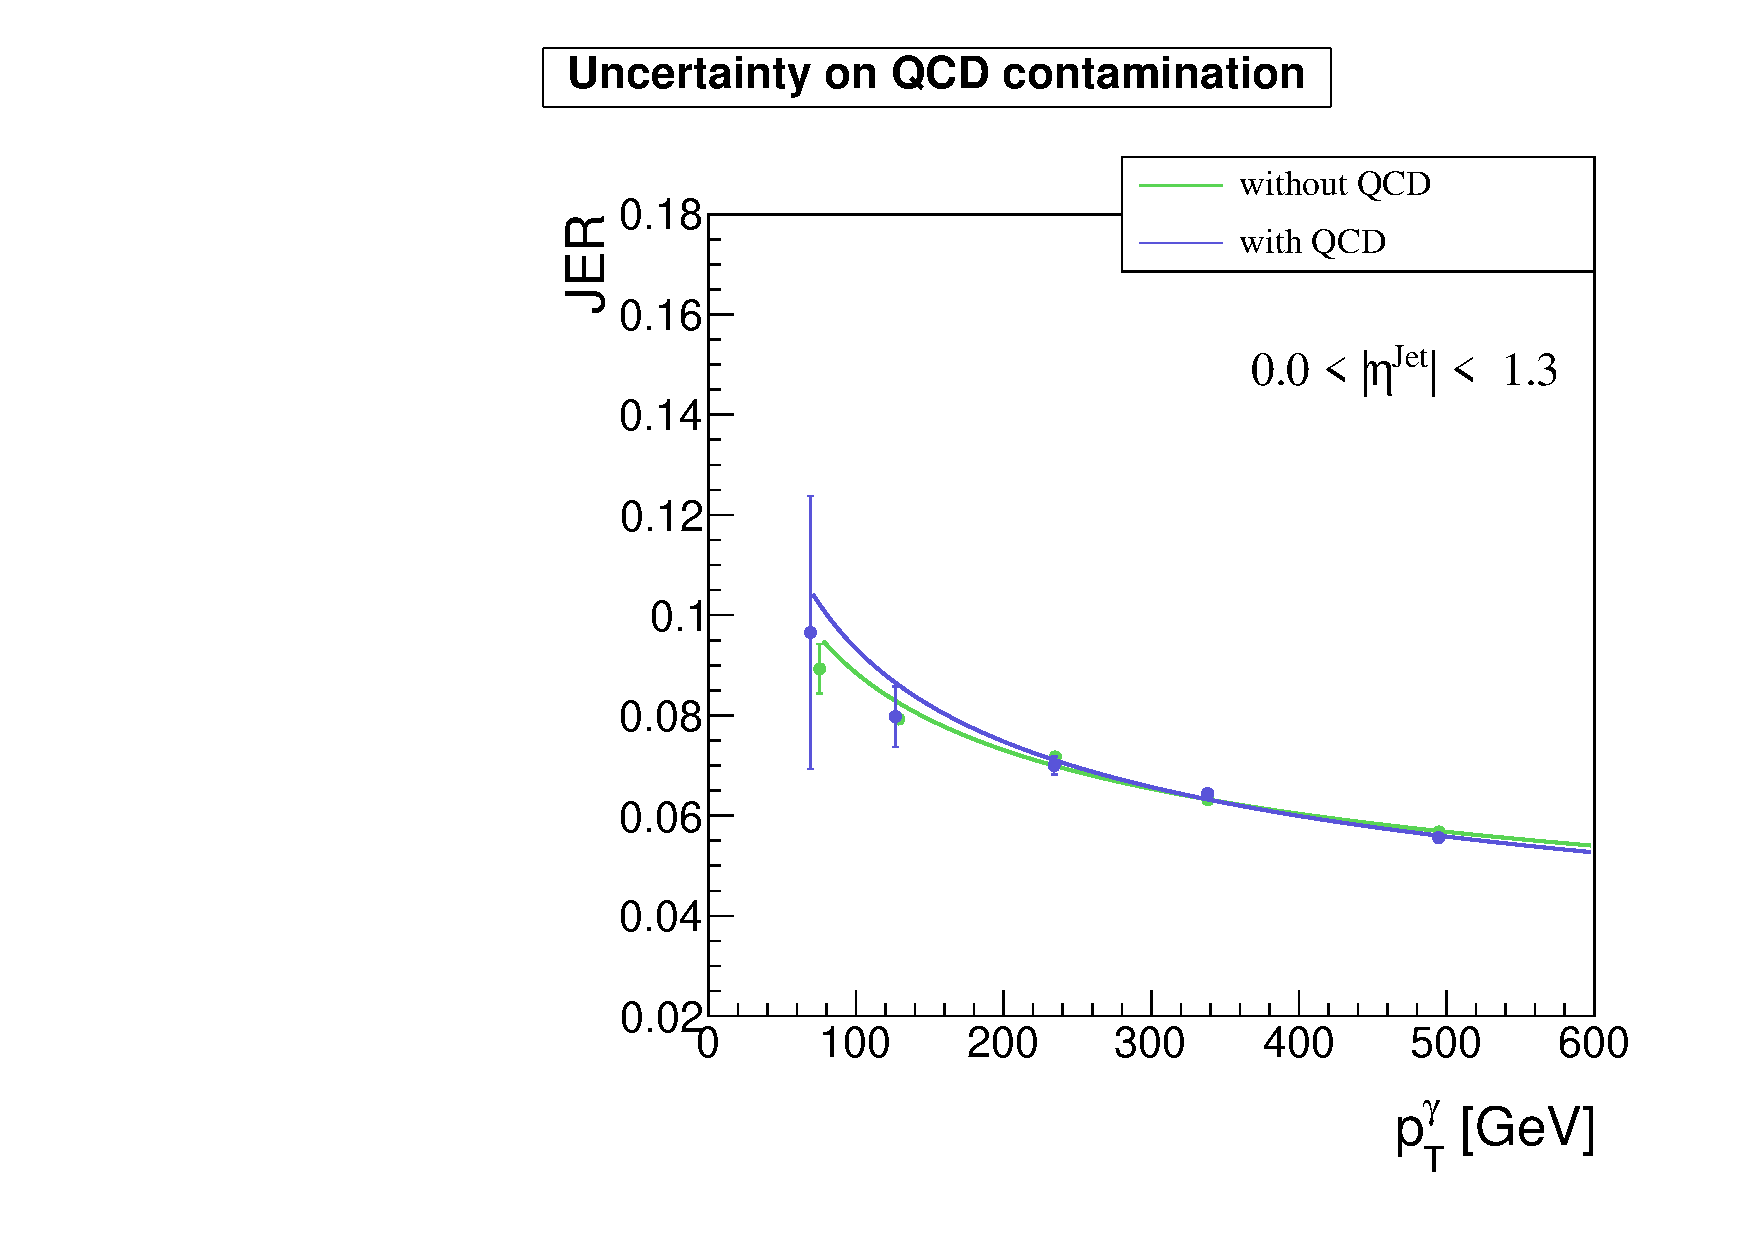
\includegraphics[width=0.50\textwidth]{figures/resolution/systematicUncertainties/Resolution_for_1_eta_bin_QCDUncertainty_RMS99.pdf}
 
  \caption{The jet energy resolution measured in simulation for $|\eta^{\text{1st jet}}| < 1.3$ with (blue) and without (green) a dijet sample added to the $\GAMJET$ sample.}  
  \label{fig:QCDuncertainty}
\end{figure}
It is obvious that the errors with the dijet sample are much larger because of the high event weights in this sample. 
Nevertheless, including a dijet sample worsens the resolution for small $\pt^{\gamma}$ and improves it slightly for high $\pt^{\gamma}$.

To estimate the impact on the data to simulation ratio, 
the photon \pt dependent  relative difference 

\begin{equation}
\label{eq:dijetUnc1}
\delta^{\text{dijet}} \left( \pt^{\gamma} \right) \left(= \frac{\text{f}_{\text{with QCD}}}{\text{f}_{\text{without QCD}}} - 1 \right)
\end{equation}
 
between the fitted curves in \mbox{Fig. \ref{fig:QCDuncertainty}}
was determined  , and the data measurement was scaled by it for every $\pt^{\gamma}$ bin 

\begin{equation}
\label{eq:dijetUnc}
\frac{\text{JER}^{\text{data}}}{\text{JER}^{\text{MC}}}^{\text{Up/Down}} \left( \pt^{\gamma}   \right) = \frac{\text{JER}^{\text{data}} 
\cdot (1 \pm \delta^{\text{dijet}}\left( \pt^{\gamma} \right))}{\text{JER}^{\text{MC}}}. 
\end{equation}

The uncertainty on the final data to simulation ratio was then evaluated by redoing the horizontal fit for the upward and downward varied data to simulation ratio 
in every $\eta^{\text{1st jet}}$ bin.

%\begin{equation}
%\label{eq:dijetUncFINAL}
%\frac{\text{JER}^{\text{data}}_{\text{Up}}}{\text{JER}^{\text{MC}}} - \frac{\text{JER}^{\text{data}}_{\text{Down}}}{\text{JER}^{\text{MC}}}.
%\end{equation}

\section*{Flavor uncertainty}
A possible difference among the resolution of different jet flavors (caused by \eg more pronounced out-of-cone showering of gluon jets) 
should in principle not play a role for the data to simulation scaling factors 
$\frac{\text{JER}^{\text{data}}}{\text{JER}^{\text{MC}}}$ as long as the flavor composition
of the data and simulation samples is the same. 

To account for a possible discrepancy of the flavor composition between data and simulation, the gluon and quark flavor fractions of the simulated sample were varied by 10\%.

The usual composition in a $\GAMJET$ sample is around 60\% light quarks and 20\% to 35\% gluons (see \mbox{Fig. \ref{fig:FlavorFraction}}). 
The missing fraction is mainly made up out of charm quarks. 
\begin{figure}[b]
  \centering

      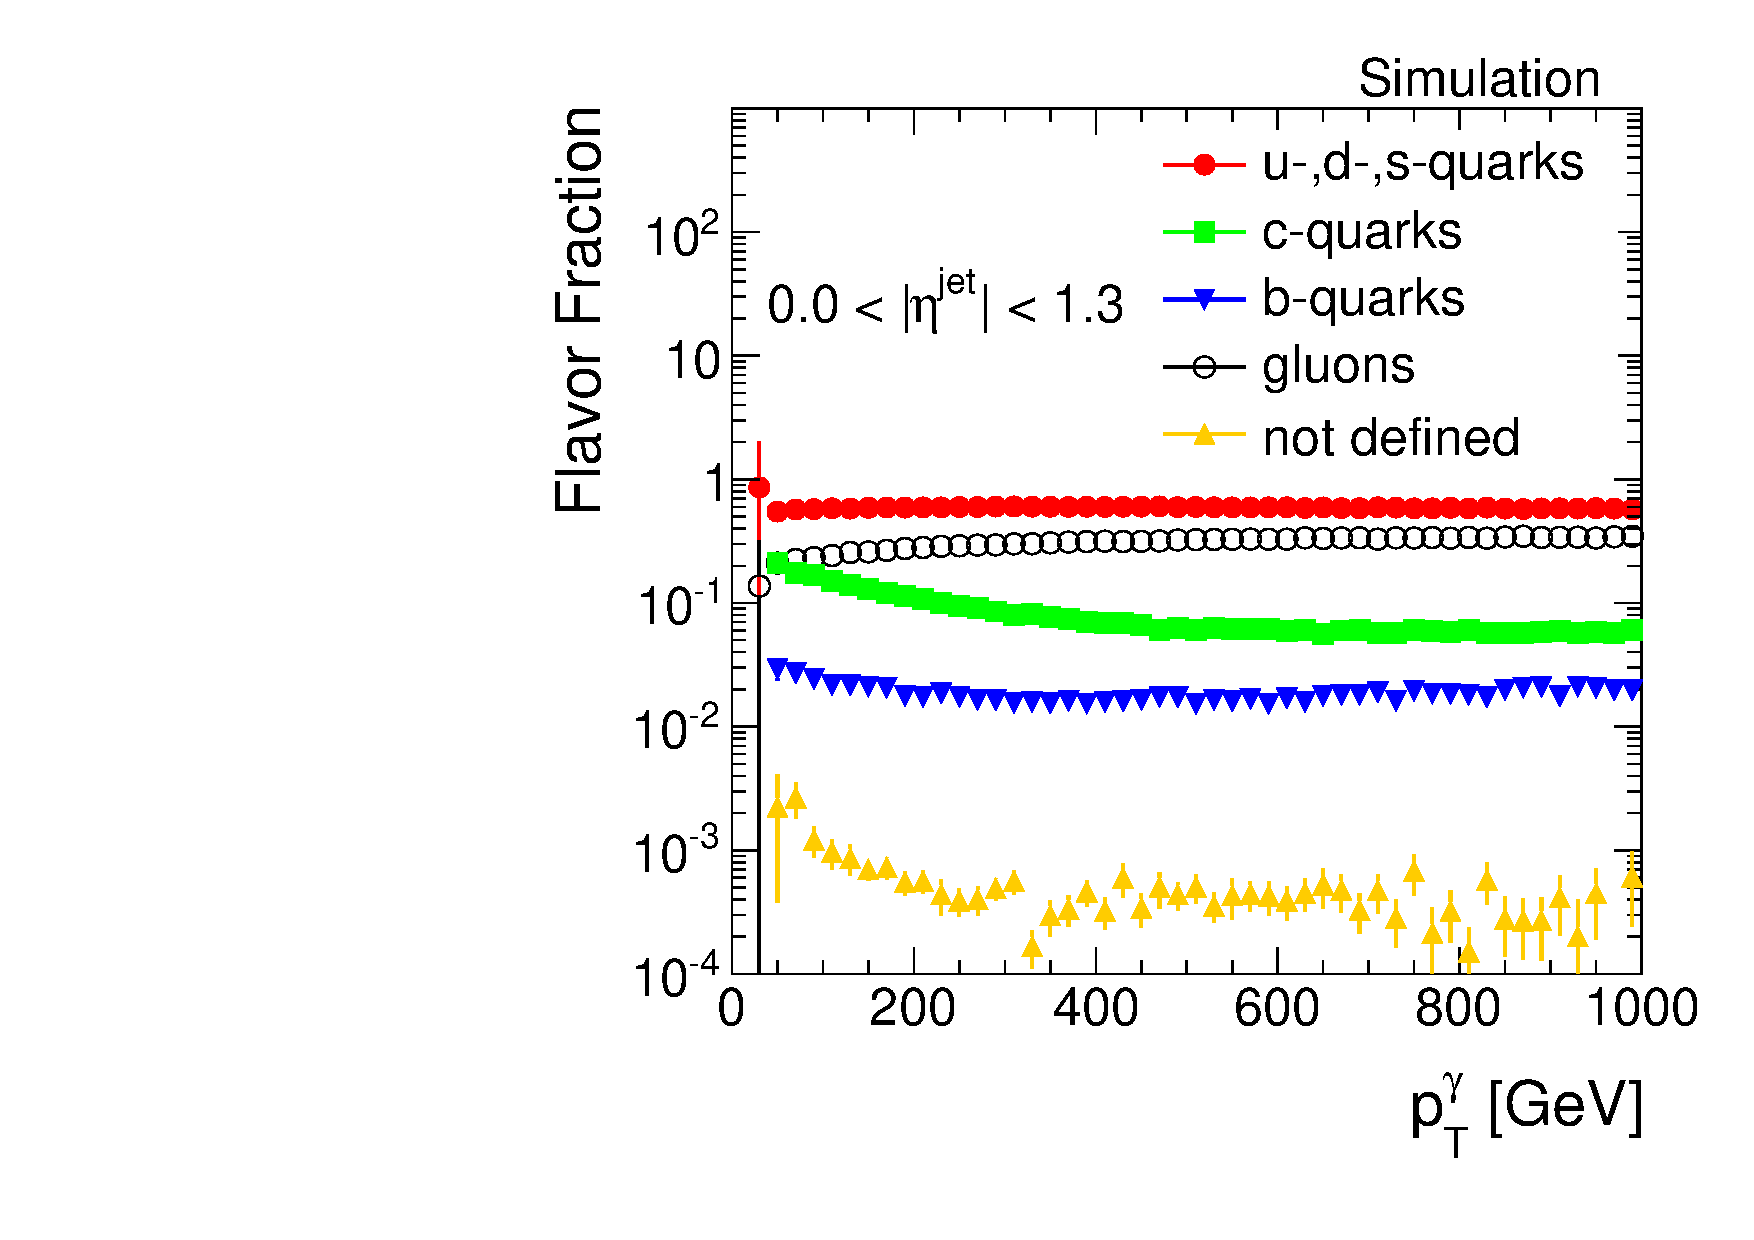
\includegraphics[width=0.50\textwidth]{figures/resolution/systematicUncertainties/flavorFraction_barrel_algo.pdf}
 
  \caption{The flavor composition of the $\GAMJET$ sample in the barrel region of the detector. 
           The algorithmic flavor definition was used (see appendix \ref{app:systematics} for more details).}  
  \label{fig:FlavorFraction}
\end{figure}

To estimate the effect of the flavor uncertainty, the intrinsic resolution in simulation was separately evaluated for quarks (JER$_\text{quarks}$) and gluons (JER$_\text{gluons}$). 
The separation between the different flavors was done using the algorithmic flavor definition (see appendix \ref{app:systematics} for more details about this definition).
\mbox{Figure \ref{fig:ResolutionDifferences}} shows the differences in resolution for all flavors separately for one exemplary $\eta$-bin.
\begin{figure}[tp]
  \centering

      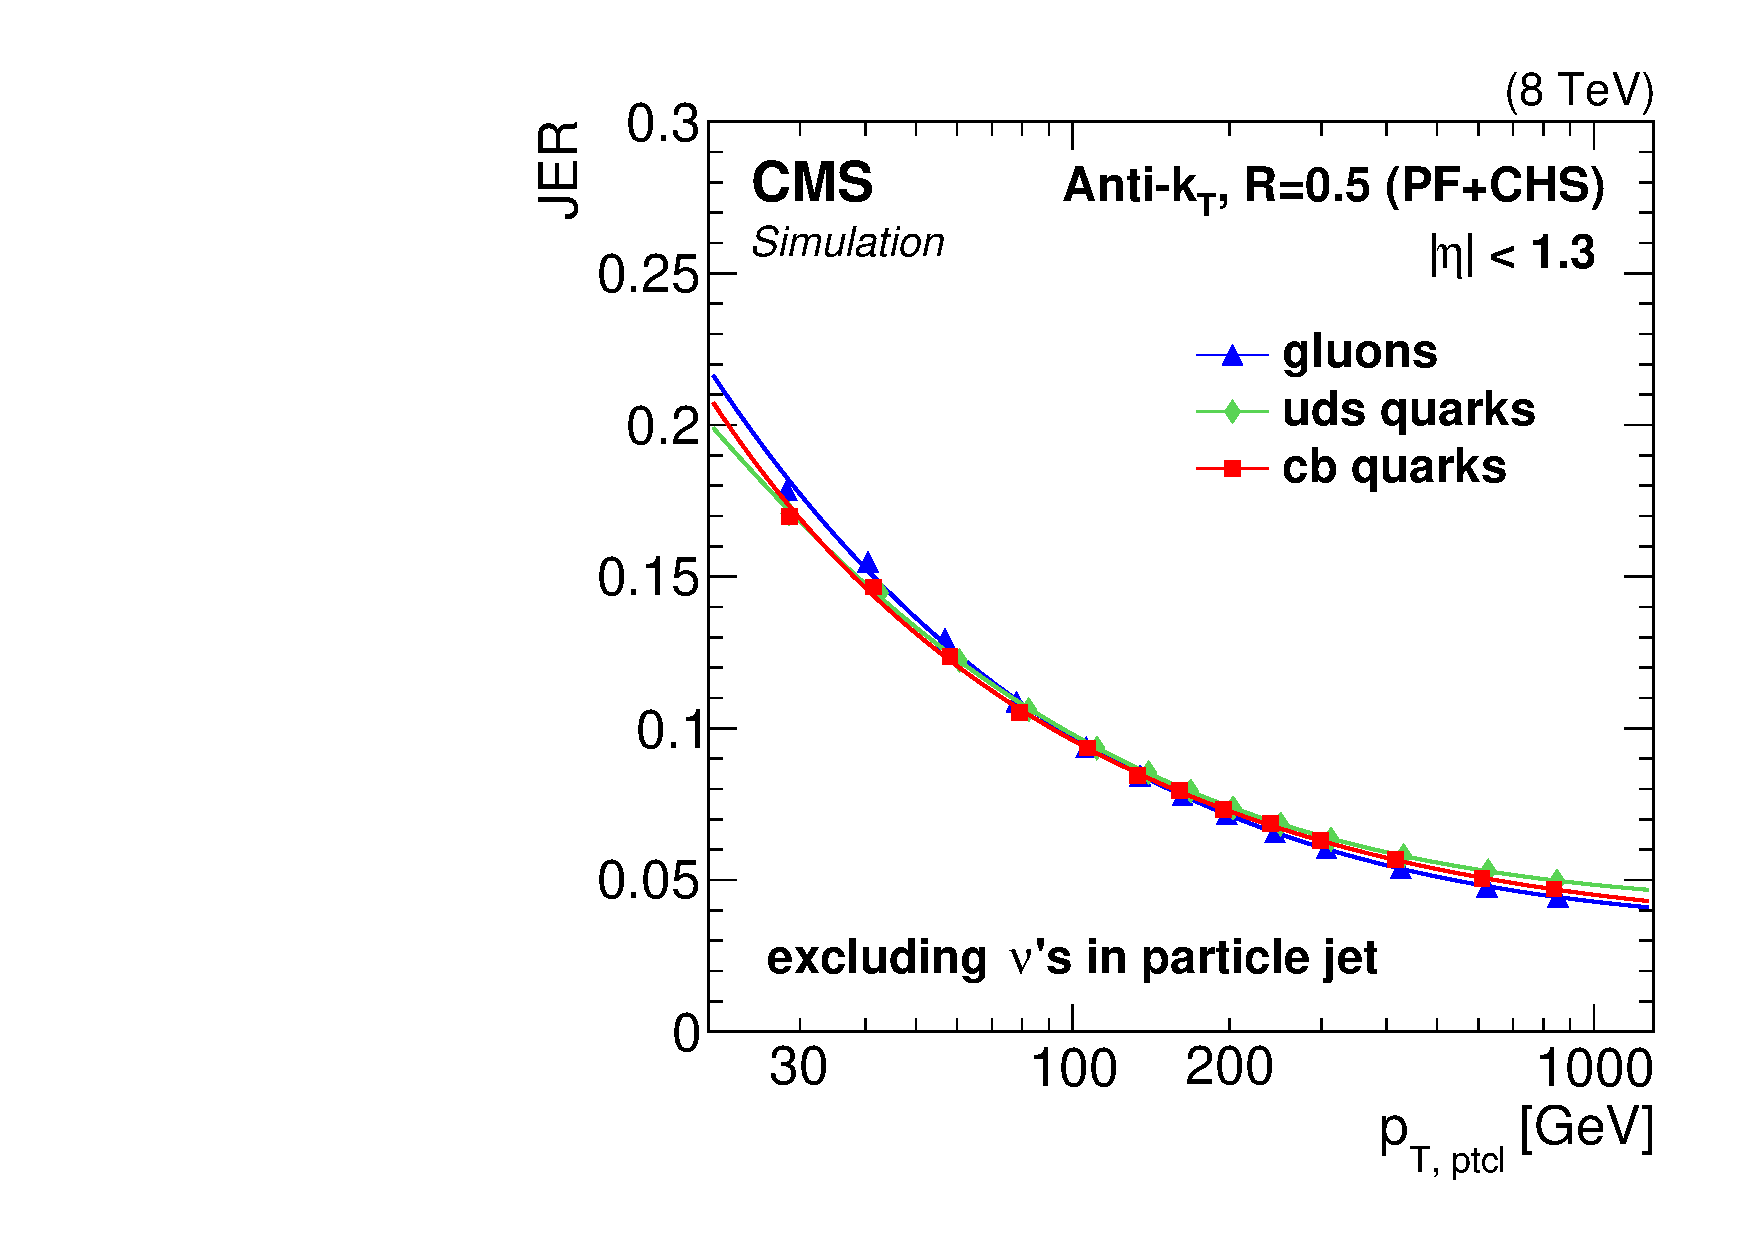
\includegraphics[width=0.50\textwidth]{figures/resolution/systematicUncertainties/Resolution_for_1_eta_bin_FlavorUncertainty_RMS99.pdf}
 
  \caption{The intrinsic resolution for $|\eta^{\text{1st jet}}| < 0.5$ for the different jet flavors.}  
  \label{fig:ResolutionDifferences}
\end{figure}
The resolution for gluon and light quark jets is comparable for small $\pt^{\gamma}$ and gets larger for high $\pt^{\gamma}$.
The energy of possible neutrinos is counted into the generator jet \pt. 
The intrinsic resolution of charm and bottom quarks is therefore shifted to larger values compared to the light quark resolution.

%The weighted mean of the quark and the gluon resolution was then taken to estimate the resolution for a different flavor composition, with weights of 
%$\frac{\text{\#quarks/\#gluons}}{\text{\#quarks+\#gluons}} \pm 0.1$. 

The weighted mean of the quark and the gluon resolution was then taken to estimate the resolution for a different flavor composition, 
with the weights (binned in $\eta^{\text{1st jet}}$ and $\pt^{\gamma}$) 
corresponding to the fraction of events with leading gluon jets or leading quark jets and the desired variation of the flavor fraction of 10\% 

\begin{equation}
\label{FlavorWeights}
 \text{weight}^{\text{Up/Down}}_{\text{gluons/quarks}} \left(\eta^{\text{1st jet}},\pt^{\gamma} \right) = \frac{\int\text{events(1st jet = gluon/quark jet)}}{\int\text{ all events}} \pm 0.1.
\end{equation}

The estimated upper and lower resolution was taken as

\begin{equation}
\label{FlavorError}
 \text{JER}^{\text{Up/Down}}_{\text{Flavor}} \left(\eta^{\text{1st jet}},\pt^{\gamma} \right) = \text{weight}^{\text{Down/Up}}_{\text{gluons}}\cdot\text{JER}_\text{gluons} +  \text{weight}^{\text{Up/Down}}_{\text{quarks}}\cdot\text{JER}_\text{quarks},  
\end{equation}
 
with both weights adding up to one.
The relative difference to the intrinsic resolution evaluated on the full sample is shown in \mbox{Fig. \ref{fig:FlavorUncertainty}} for the first $\eta^{\text{1st jet}}$ bin 
(see Appendix \ref{subsecApp:flavor} for all plots).
\begin{figure}[b]
  \centering

      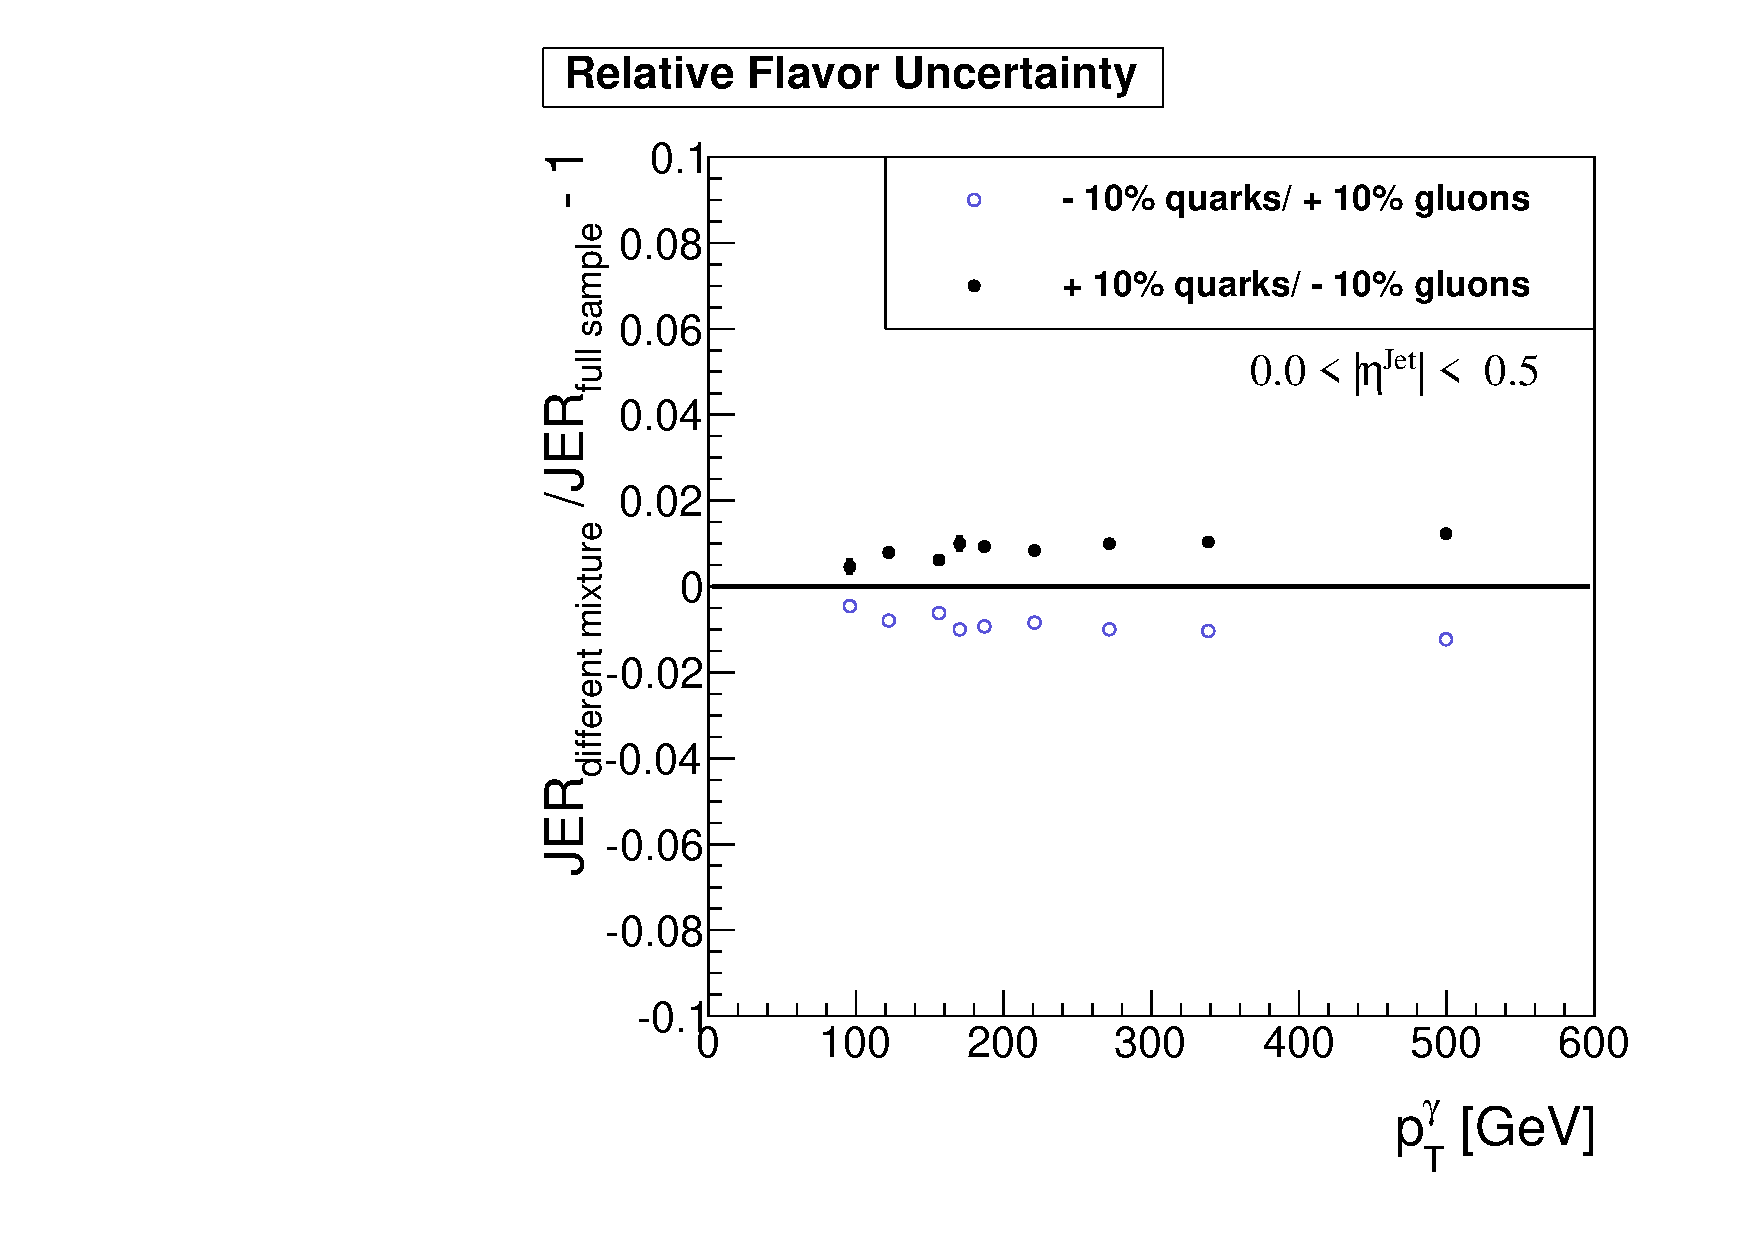
\includegraphics[width=0.50\textwidth]{figures/resolution/systematicUncertainties/Relative_Resolution_for_1_eta_bin_FlavorUncertainty_RMS99_mixture.pdf}
 
  \caption{The relative differences $\left( \delta^{\text{Flavor}}_{\text{Up/Down}}  \left(\eta^{\text{1st jet}},\pt^{\gamma} \right)\right)$ 
           between the weighted intrinsic resolution and the real intrinsic resolution for $|\eta^{\text{1st jet}}| < 0.5$.}  
  \label{fig:FlavorUncertainty}
\end{figure}  
%The error bars in \mbox{Fig. \ref{fig:FlavorUncertainty}} are calculated taken the correlation between the full sample and the gluon and the quark subsamples into account with 
%the correlation coefficient
%\begin{equation}
%\label{FlavorCorrelation}
%\rho = \frac{\int\text{events(1st jet = gluon/quark jet)}}{\int\text{ all events}}. 
%\end{equation}
These relative differences were used to scale the simulation resolution up and down in every $\pt^{\gamma}$ bin

\begin{equation}
\label{FlavorUpDown}
\text{JER}^{\text{MC}}_{\text{Up/Down}} \left(\pt^{\gamma} \right) = \text{JER}^{\text{MC}} \left(\pt^{\gamma} \right) \cdot \left(1 + \delta^{\text{Flavor}}_{\text{Up/Down}}  \left(\eta^{\text{1st jet}},\pt^{\gamma} \right) \right).
\end{equation}

Then the constant fit to the data to simulation ratio $\frac{\text{JER}^{\text{data}}}{\text{JER}^{\text{MC}}}$ was reevaluated and 
the final relative systematic uncertainty is thus 

\begin{equation}
\label{FlavorUncFINAL}
\delta \left( \frac{\text{JER}^{\text{data}}}{\text{JER}^{\text{MC}}} \right)^{\text{Flavor}} = \frac{\text{const. fit}^{\text{varied mixture in MC}}}{\text{const. fit}^{\text{original mixture in MC}}} - 1.
\end{equation}

%%%%%%%%%%%%%%%%%%%%%%%%%%%%%%%%%%%%%%%%%%%%%%%%%%%%%%%%%%%%%%%%%%%%%%%%%%%%%%%%%%%%%%%%%%%%%%%%%%%%%%%%%%%%%%%%%%%%%%%%%%%%%%%%%%%%%%%%%%%%%%%%%%%%%%%%%%%%%%%%%%%%%%%%%%%%%%%%%%%%%%%%%%%%%%%%%%%%%%%%%%%%%%%%%%%%%%%%%%%%%%%%%%%%%%%%%%%
\section*{Out-of-Cone showering uncertainty}
Another source of uncertainty is the use of MC-truth information by taking the residual imbalance $q^{\prime}$ from simulation as input to the fitted data resolution 
\mbox{(Eq.~\eqref{eq:total})}.

It is not clear whether out-of-cone showering is really well modeled in simulation. 
Therefore, to account for possible differences between the real and the simulated out-of-cone showering, the ratio $\frac{\text{JER}^{\text{data}}}{\text{JER}^{\text{MC}}}$ 
was evaluated with different jet radii of the jet reconstruction algorithm. 

For the primary analysis, jets reconstructed by the Anti-k$_{\text{t}}$ algorithm with a radius of 0.5 were used (AK5 jets). 
To evaluate the systematic uncertainty, the whole analysis was redone with jets reconstructed with a jet radius of 0.7 (AK7 jets). 
\mbox{Figure \ref{fig:ak5ak7}} shows the evaluated ratio $\frac{\text{JER}^{\text{data}}}{\text{JER}^{\text{MC}}}$  
for the two different jet collections in two  exemplary $\eta$-bins. 
\begin{figure}[b]
 \centering
     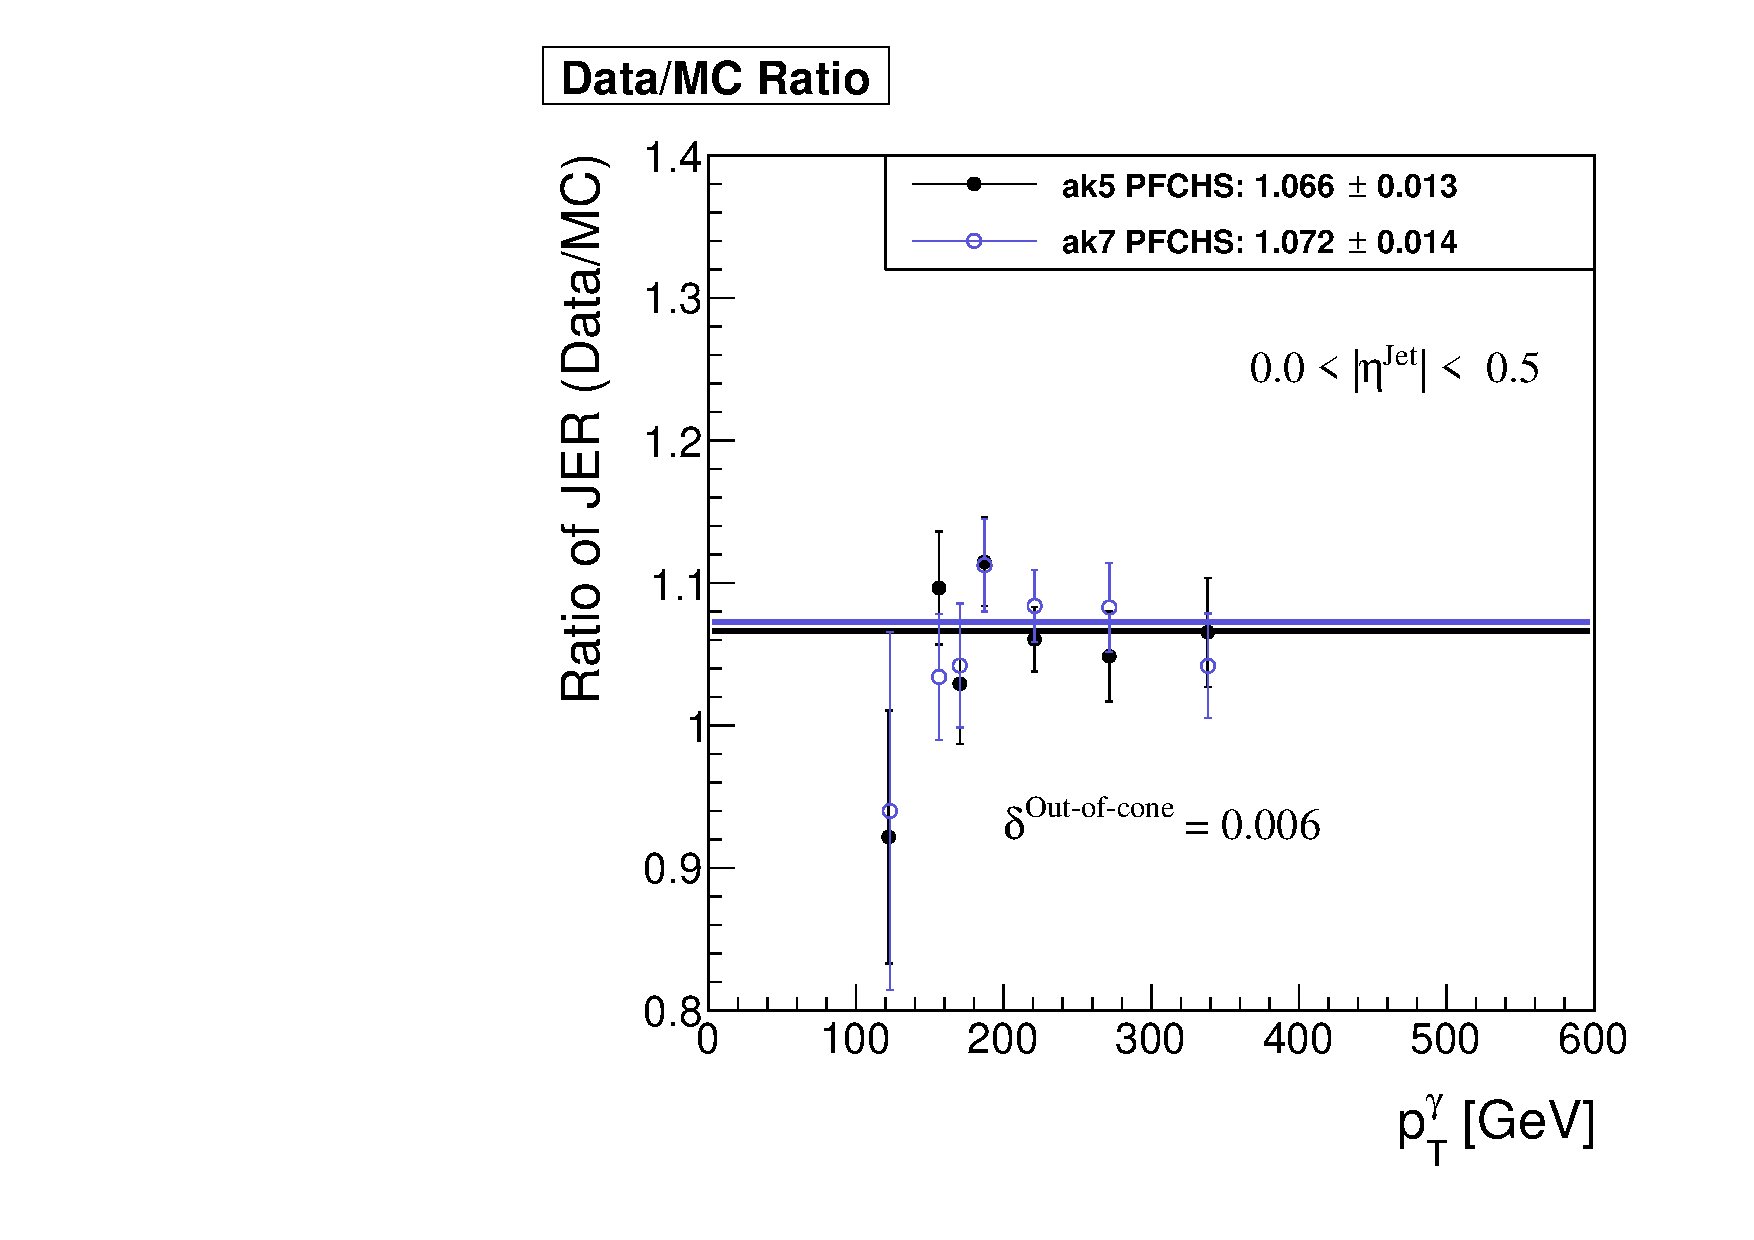
\includegraphics[width=0.49\textwidth]{figures/resolution/systematicUncertainties/Ratio_Resolution_for_1_eta_bin_PFCHS_RMS99_ak5_ak7_comparison.pdf}
    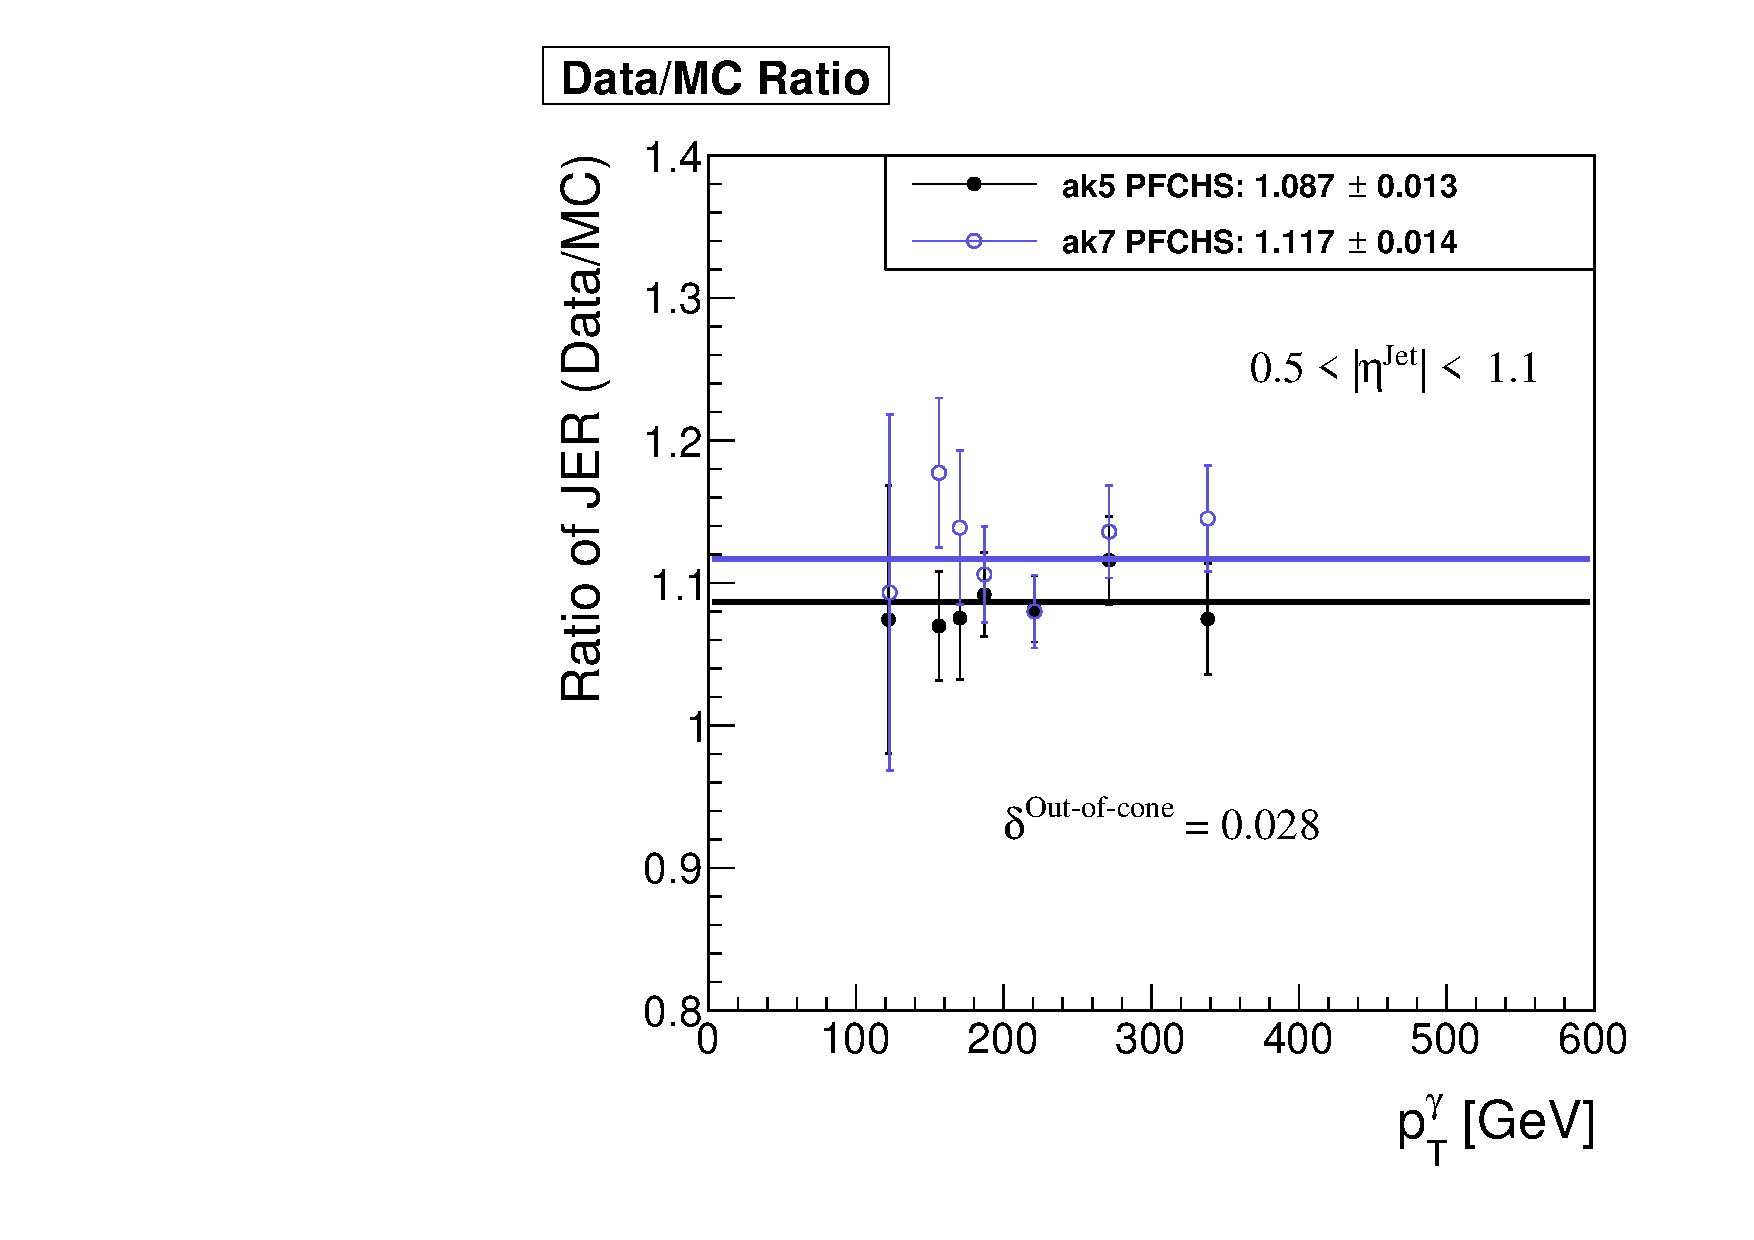
\includegraphics[width=0.49\textwidth]{figures/resolution/systematicUncertainties/Ratio_Resolution_for_2_eta_bin_PFCHS_RMS99_ak5_ak7_comparison.pdf}
  \caption{The data to simulation ratio $\frac{\text{JER}^{\text{data}}}{\text{JER}^{\text{MC}}}$ 
           using Anti-k$_{\text{t}}$ jets with jet radius of 0.5 (black) and jet radius of 0.7 (blue) for two different $\eta^{\text{1st jet}}$ bins: 
           left:  $0.0<|\eta^{\text{1st jet}}|<0.5$, right: $0.5<|\eta^{\text{1st jet}}|<1.1$}
 \label{fig:ak5ak7}
\end{figure}
The statistical uncertainties are mainly coming from the limited statistical precision of the data sample. 
Thus, reducing the significance of the systematic difference between the data to simulation ratio of  AK5 and AK7 jets.
Still, the data to simulation ratio is in all $\eta$ bins larger for the AK7 jets (see Appendix \ref{subsecApp:mc}).

The relative difference $\delta^{\text{Out-of-cone}}$ between the constant fit of $\frac{\text{JER}^{\text{data}}}{\text{JER}^{\text{MC}}}$ using AK5 jets and using 
AK7 jets in every $\eta^{\text{1st jet}}$ bin was taken as upward and downward systematic uncertainty of the resolution ratio

\begin{equation}
\label{MCUncFINAL}
\pm \delta \left( \frac{\text{JER}^{\text{data}}}{\text{JER}^{\text{MC}}} \right) = \pm \delta^{\text{Out-of-cone}} = \frac{\text{const. fit}_{\text{AK7}}}{\text{const. fit}_{\text{AK5}}} - 1.
%\pm \delta \left( \frac{\text{JER}^{\text{data}}}{\text{JER}^{\text{MC}}} \right) = \pm \frac{\text{JER}^{\text{data}}}{\text{JER}^{\text{MC}}} \cdot \left(1 + \delta^{\text{Out-of-cone}}  \right).
\end{equation}

%%%%%%%%%%%%%%%%%%%%%%%%%%%%%%%%%%%%%%%%%%%%%%%%%%%%%%%%%%%%%%%%%%%%%%%%%%%%%%%%%%%%%%%%%%%%%%%%%%%%%%%%%%%%%%%%%%%%%%%%%%%%%%%%%%%%%%%%%%%%%%%%%%%%%%%%%%%%%%%%%%%%%%%%%%%%%%%%%%%%%%%%%%%%%%%%%%%%%%%%%%%%%%%%%%%%%%%%%%%%%%%%%%%%%%%%%%%
\section*{Jet energy correction uncertainty}
Another source of uncertainty arises from the jet energy correction factors.
These serve to correct the measured jet \pt to the particle-level \pt.

The correction factors are mainly determined with the help of simulated data samples but are also applied to measured data. 
Therefore, there is an uncertainty of how well the correction factors in data and simulation agree.

To determine the effect on the resolution ratio, all jets in the simulated data sample were varied up and down by this uncertainty 
($p^{\text{jet}}_{\text{T up/down}} = \pt^{\text{jet}} \cdot (1 \pm \Delta_{\text{JEC}})$).
The whole analysis was then redone in simulation and the relative difference between the intrinsic result of JER$_{\text{intrinsic}}$($\pt^{\gamma}$) 
for the varied sample and the original value of JER$_{\text{intrinsic}}$($\pt^{\gamma}$)
was evaluated.
In \mbox{Fig. \ref{fig:JECUncertainty}} the relative differences are shown for the first $\eta^{\text{1st jet}}$ bin (see Appendix \ref{subsecApp:JEC} for all plots).


\begin{figure}[b]
  \centering
      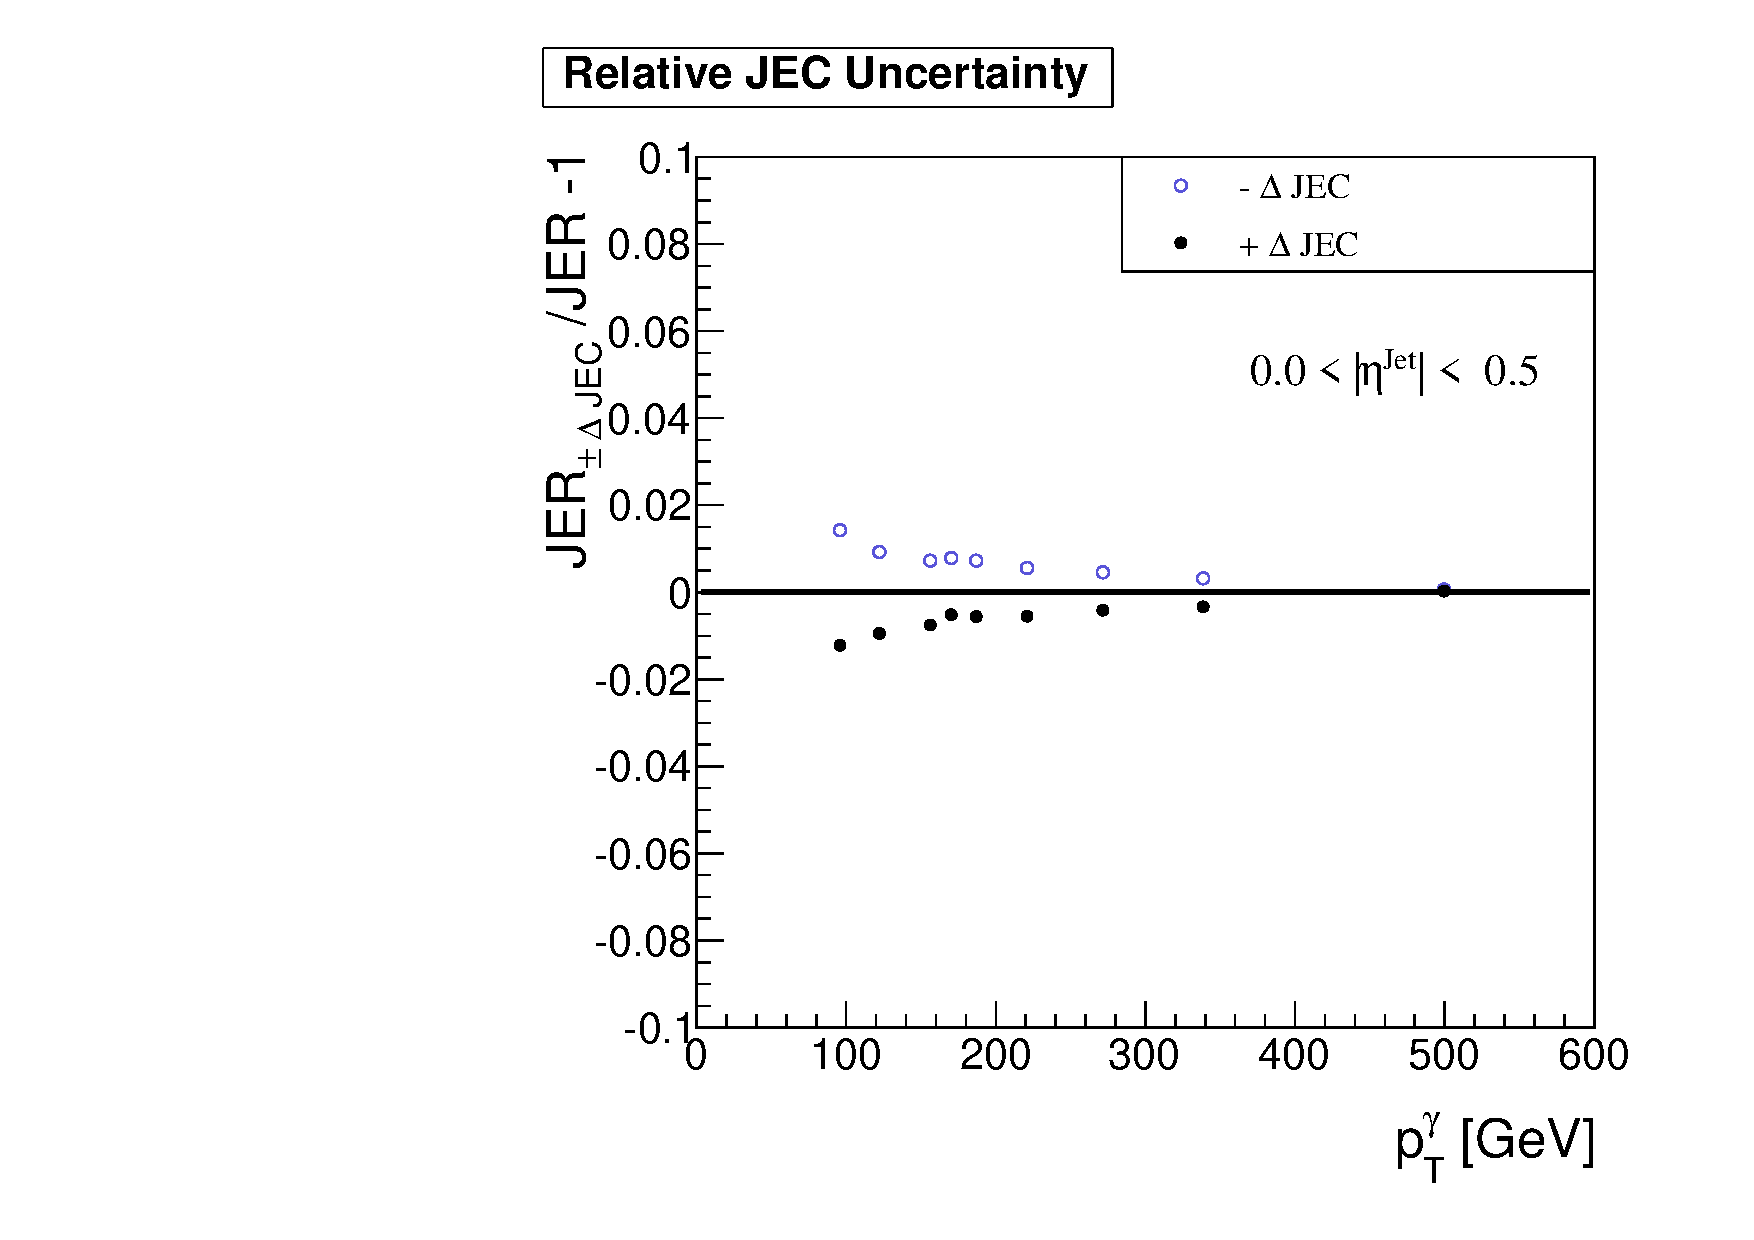
\includegraphics[width=0.50\textwidth]{figures/resolution/systematicUncertainties/Relative_Resolution_for_1_eta_bin_JECUncertainty_RMS99.pdf}
   \caption{The relative difference between the intrinsic resolution of the simulation with all jet \pt varied up and down by the jet energy correction factors 
           and the nominal intrinsic resolution result for \mbox{$|\eta^{\text{1st jet}}| < 0.5$.}}  
  \label{fig:JECUncertainty}
\end{figure}

The evaluation of the systematic uncertainty of the data to simulation ratio was done equivalent to the flavor uncertainty estimation. 
The resulting relative differences were used to vary the simulation results up and down and the constant fit to the data to simulation ratio
$\frac{\text{JER}^{\text{data}}}{\text{JER}^{\text{MC}}}$ was redone. The final systematic uncertainty on the ratio is 

\begin{equation}
\label{JECUncFINAL}
\delta \left( \frac{\text{JER}^{\text{data}}}{\text{JER}^{\text{MC}}} \right)^{\text{JEC}} = \frac{\text{const. fit}^{1 \pm \Delta_{\text{JEC}}}}{\text{const. fit}^{\text{original}}} - 1.
\end{equation}

%%%%%%%%%%%%%%%%%%%%%%%%%%%%%%%%%%%%%%%%%%%%%%%%%%%%%%%%%%%%%%%%%%%%%%%%%%%%%%%%%%%%%%%%%%%%%%%%%%%%%%%%%%%%%%%%%%%%%%%%%%%%%%%%%%%%%%%%%%%%%%%%%%%%%%%%%%%%%%%%%%%%%%%%%%%%%%%%%%%%%%%%%%%%%%%%%%%%%%%%%%%%%%%%%%%%%%%%%%%%%%%%%%%%%%%%%%%
\section*{Pileup uncertainty}
Finally, an uncertainty due to the adjustment of the simulated events to the pileup distribution in data was evaluated.

To account for this uncertainty, the effect of a 5.0\% up- and downward variation of the minimum bias cross section (69.4 mb) 
on the resolution was evaluated, following the official recipe \mbox{in \cite{website:PileupSystematicErrors}}.
The resulting intrinsic resolution in simulation was then compared to the central resolution using the original pileup weights.
\mbox{Fig. \ref{fig:PUuncertainty}} shows the relative difference for one exemplary $\eta$ bin. 
The full set of plots can be found in \mbox{Appendix \ref{subsecApp:PU}}. 
Again, the simulation result was scaled by these relative uncertainties and the constant fit was reevaluated.
The relative systematic uncertainty on the ratio results in

\begin{equation}
\label{PUUncFINAL}
\delta \left( \frac{\text{JER}^{\text{data}}}{\text{JER}^{\text{MC}}} \right)^{\text{PU}} = \frac{\text{const. fit}^{\text{varied MBXS}}}{\text{const. fit}^{\text{original}}} - 1.
\end{equation}

\begin{figure}[h]
 \centering    
     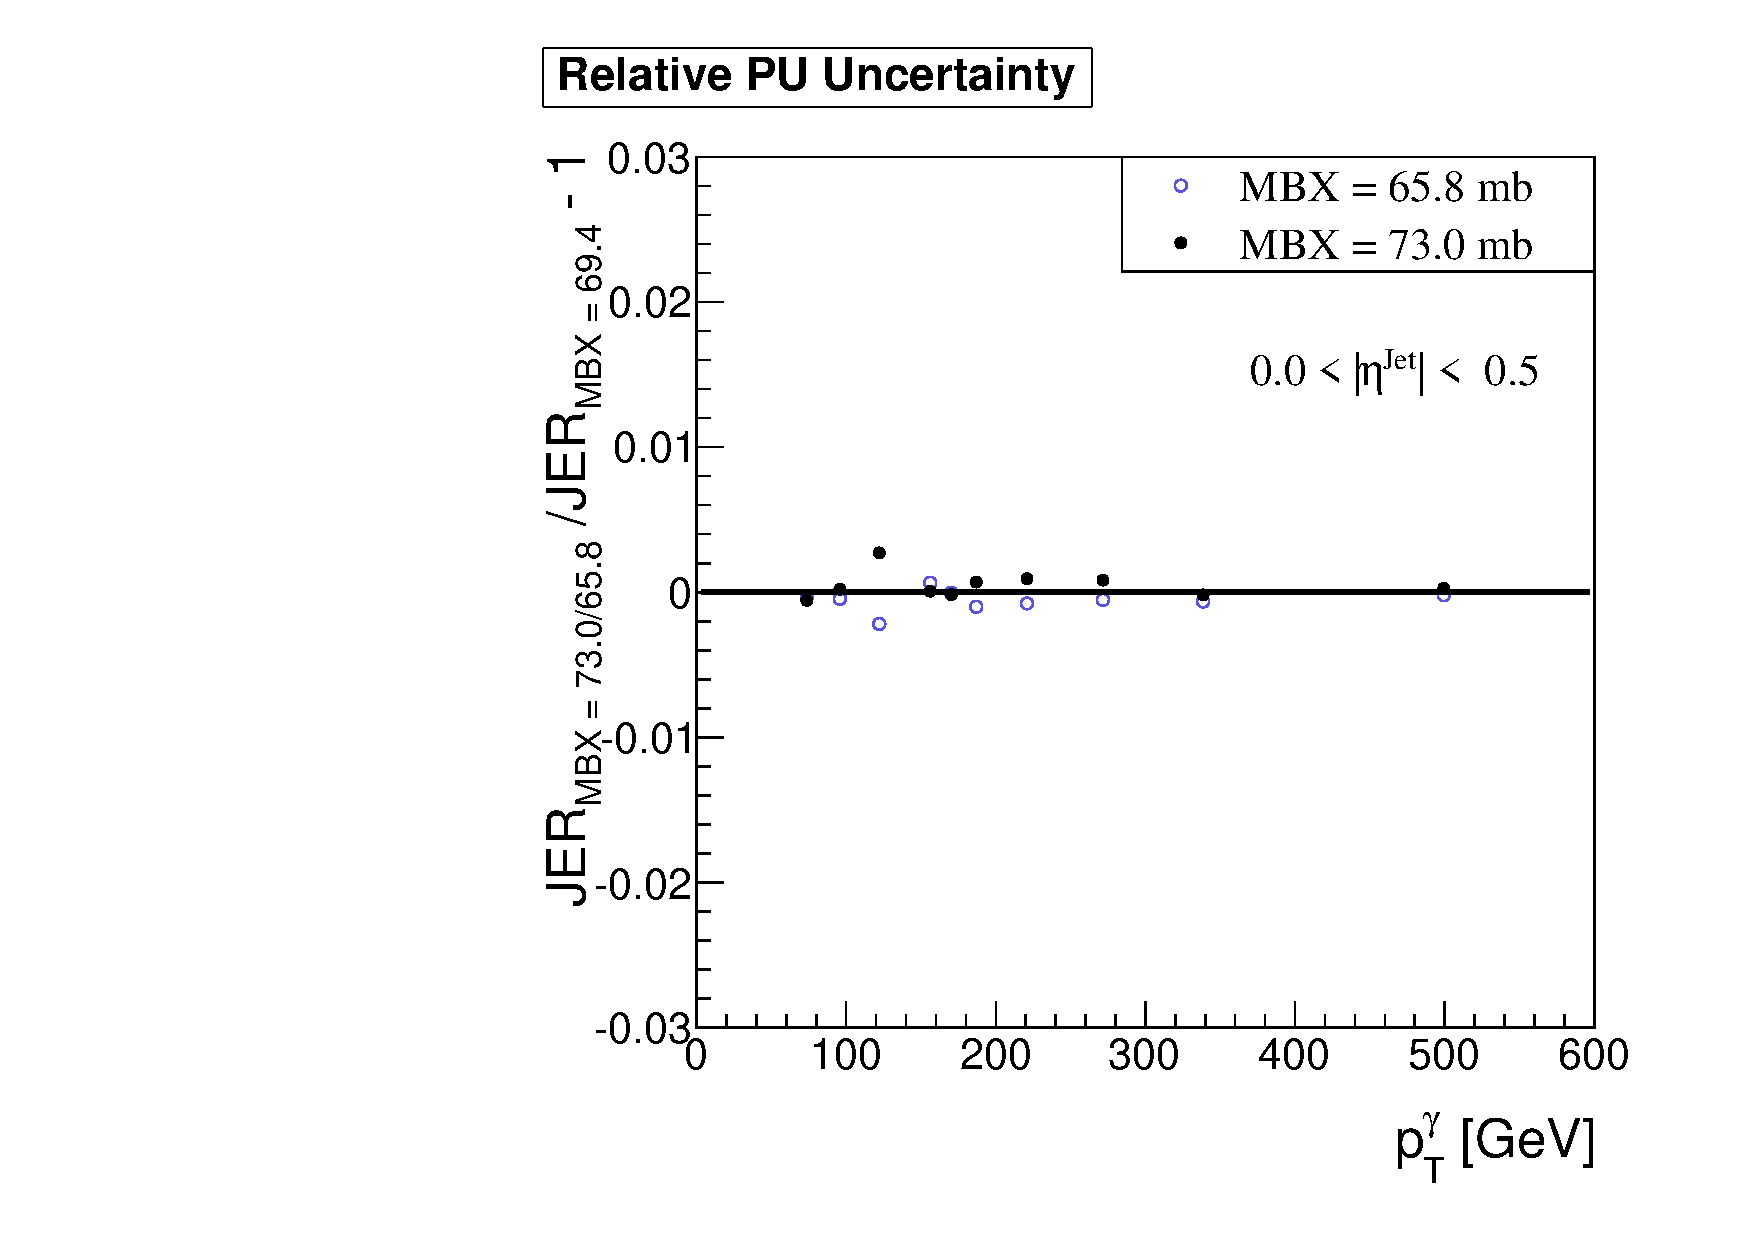
\includegraphics[width=0.50\textwidth]{figures/resolution/systematicUncertainties/Relative_Resolution_for_1_eta_bin_PUUncertainty_RMS99.pdf}
    
  \caption{Relative difference of the intrinsic resolution for different minimum bias cross sections in one exemplary $\eta^{\text{1st jet}}$ bin: 
           $0.0<\eta^{\text{1st jet}}<0.5$.}
 \label{fig:PUuncertainty}
\end{figure}


%%%%%%%%%%%%%%%%%%%%%%%%%%%%%%%%%%%%%%%%%%%%%%%%%%%%%%%%%%%%%%%%%%%%%%%%%%%%%%%%%%%%%%%%%%%%%%%%%%%%%%%%%%%%%%%%%%%%%%%%%%%%%%%%%%%%%%%%%%%%%%%%%%%%%%%%%%%%%%%%%%%%%%%%%%%%%%%%%%%%%%%%%%%%%%%%%%%%%%%%%%%%%%%%%%%%%%%%%%%%%%%%%%%%%%%%%%%

%%%%%%%%%%%%%%%%%%%%%%%%%%%%%%%%%%%%%%%%%%%%%%%%%%%%%%%%%%%%%%%%%%%%%%%%%%%%%%%%%%%%%%%%%%%%%%%%%%%%%%%%%%%%%%%%%%%%%%%%%%%%%%%%%%%%%%%%%%%%%%%%%%%%%%%%%%%%%%%%%%%%%%%%%%%%%%%%%%%%%%%%%%%%%%%%%%%%%%%%%%%%%%%%%%%%%%%%%%%%%%%%%%%%%%%%%%%
%%%%%%%%%%%%%%%%%%%%%%%%%%%%%%%%%%%%%%%%%%%%%%%%%%%%%%%%%%%%%%%%%%%%%%%%%%%%%%%%%%%%%%%%%%%%%%%%%%%%%%%%%%%%%%%%%%%%%%%%%%%%%%%%%%%%%%%%%%%%%%%%%%%%%%%%%%%%%%%%%%%%%%%%%%%%%%%%%%%%%%%%%%%%%%%%%%%%%%%%%%%%%%%%%%%%%%%%%%%%%%%%%%%%%%%%%%%
\FloatBarrier
\chapter{Results}

The data to simulation resolution scaling factors have been determined in $19.7\fbinv$ of pp collision data at $\sqrt{s} = 8 \tev$ 
with the methodology described in \mbox{Chapter~\ref{sec:methodology}}.
All extrapolation plots $\text{JER} \left( \alpha   \right)$ done for every $\pt^{\gamma}$ and $\eta^{\text{1st jet}}$ bin can be found in the appendix \ref{app:results}.

For every $\eta^{\text{jet}}$ bin, a horizontal line has been fitted to the ratio
$\frac{\text{JER}^{\text{data}}}{\text{JER}^{\text{MC}}} \left( \pt^{\gamma} \right)$.
In \mbox{Fig. \ref{fig:RatioEtaBinned}}, the results for all four $\eta^{\text{jet}}$-ranges can bee seen. 
The $\chi^2$/NDF-values for the four fits vary between 0.23 and 2.53. 
Thus, a horizontal fit is justified, and one value for every $\eta$-bin will be reported.

\begin{figure}[!b]
 \centering
    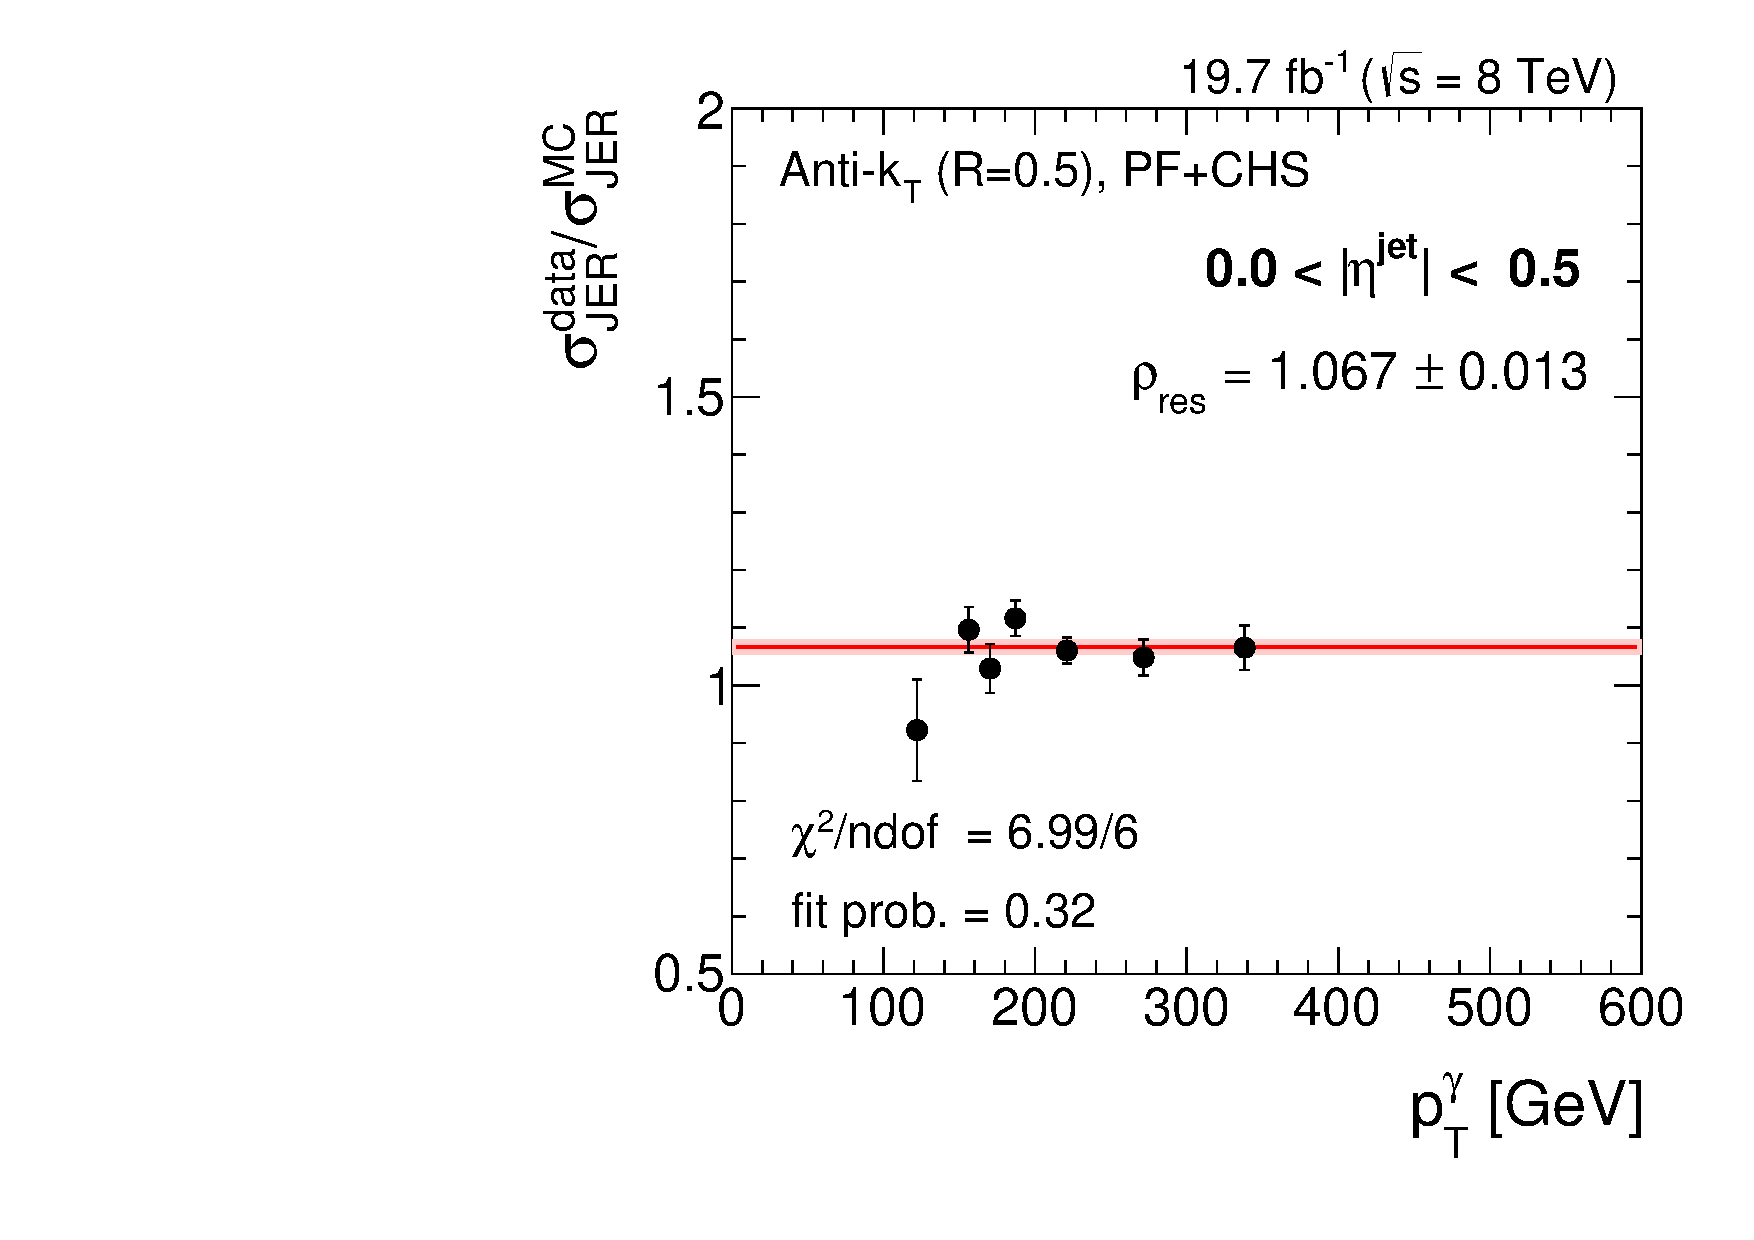
\includegraphics[width=0.49\textwidth]{figures/resolution/results/Ratio_Resolution_for_1_eta_bin_PFCHS_data_comparison_RMS99.pdf}
    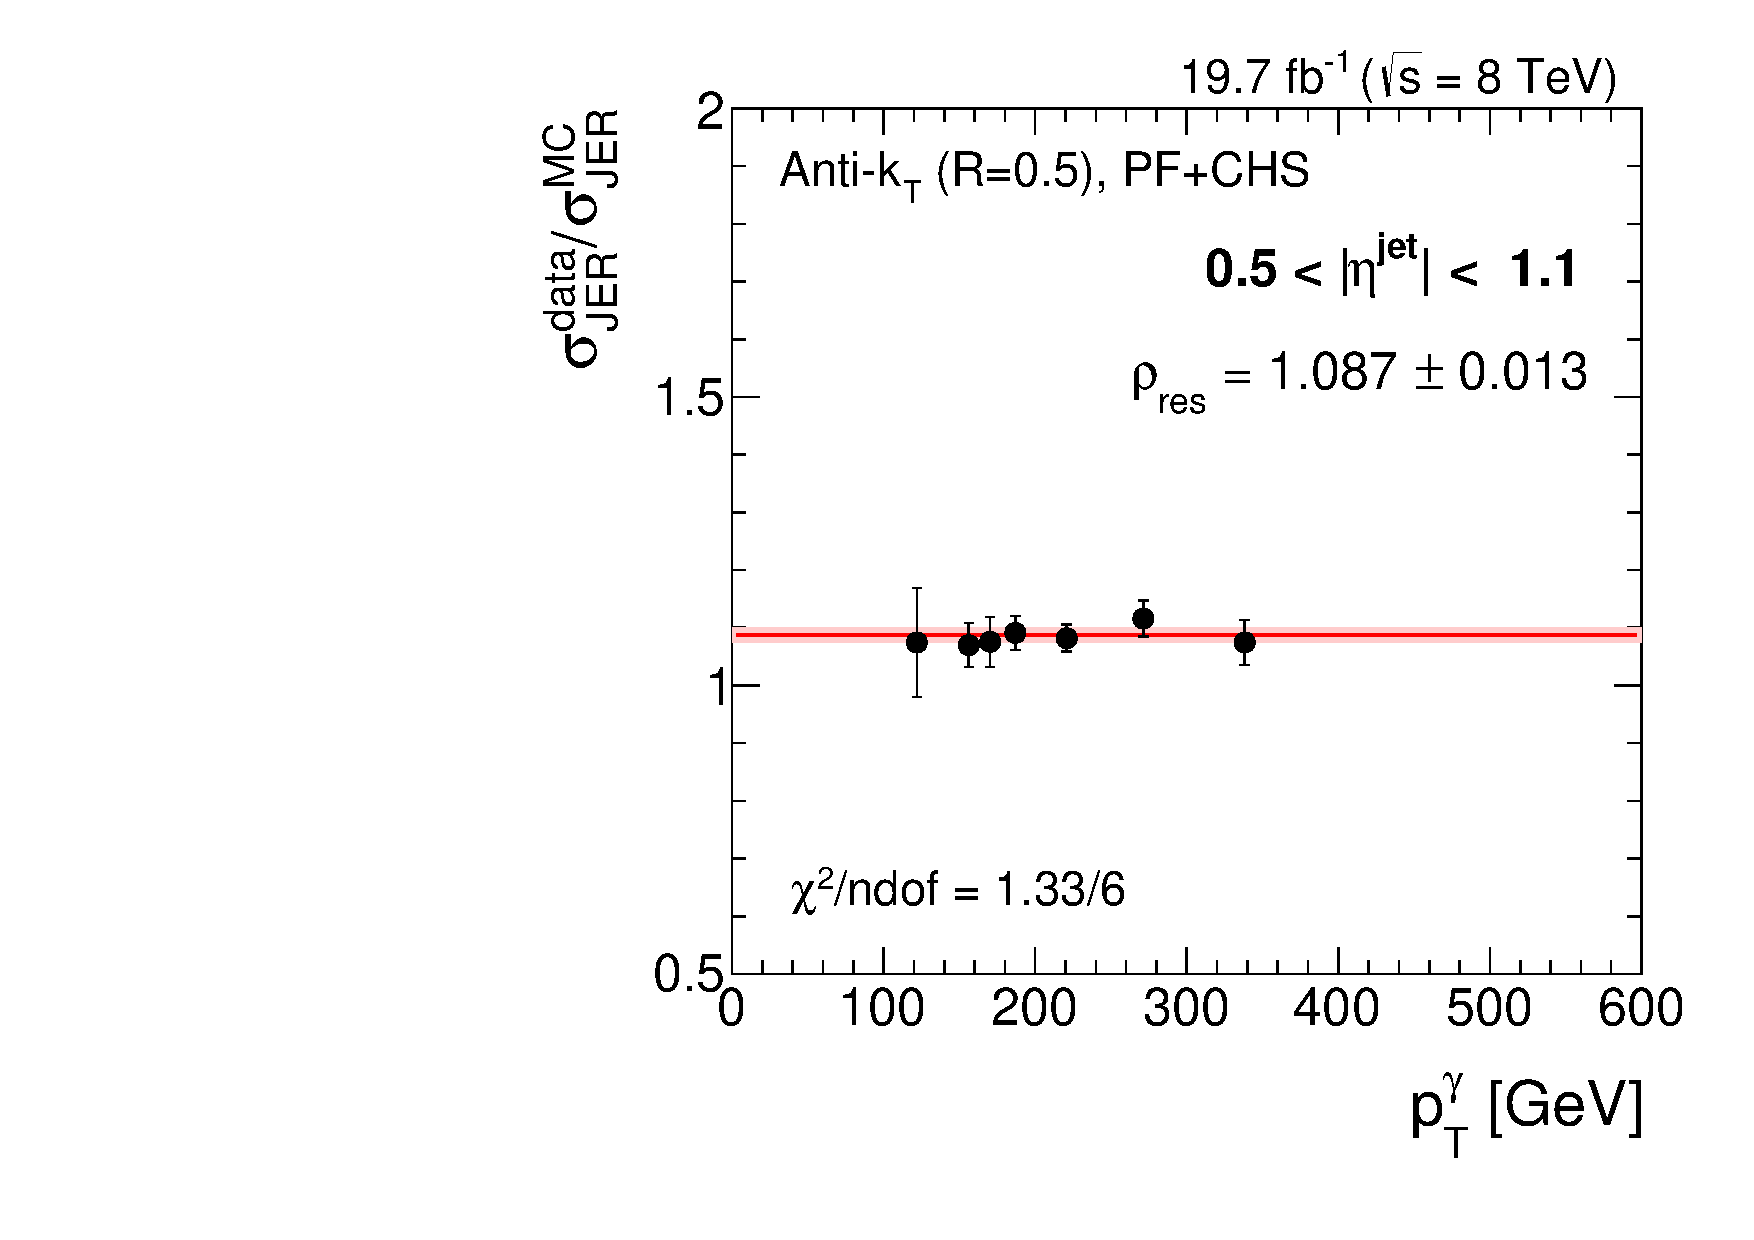
\includegraphics[width=0.49\textwidth]{figures/resolution/results/Ratio_Resolution_for_2_eta_bin_PFCHS_data_comparison_RMS99.pdf}

    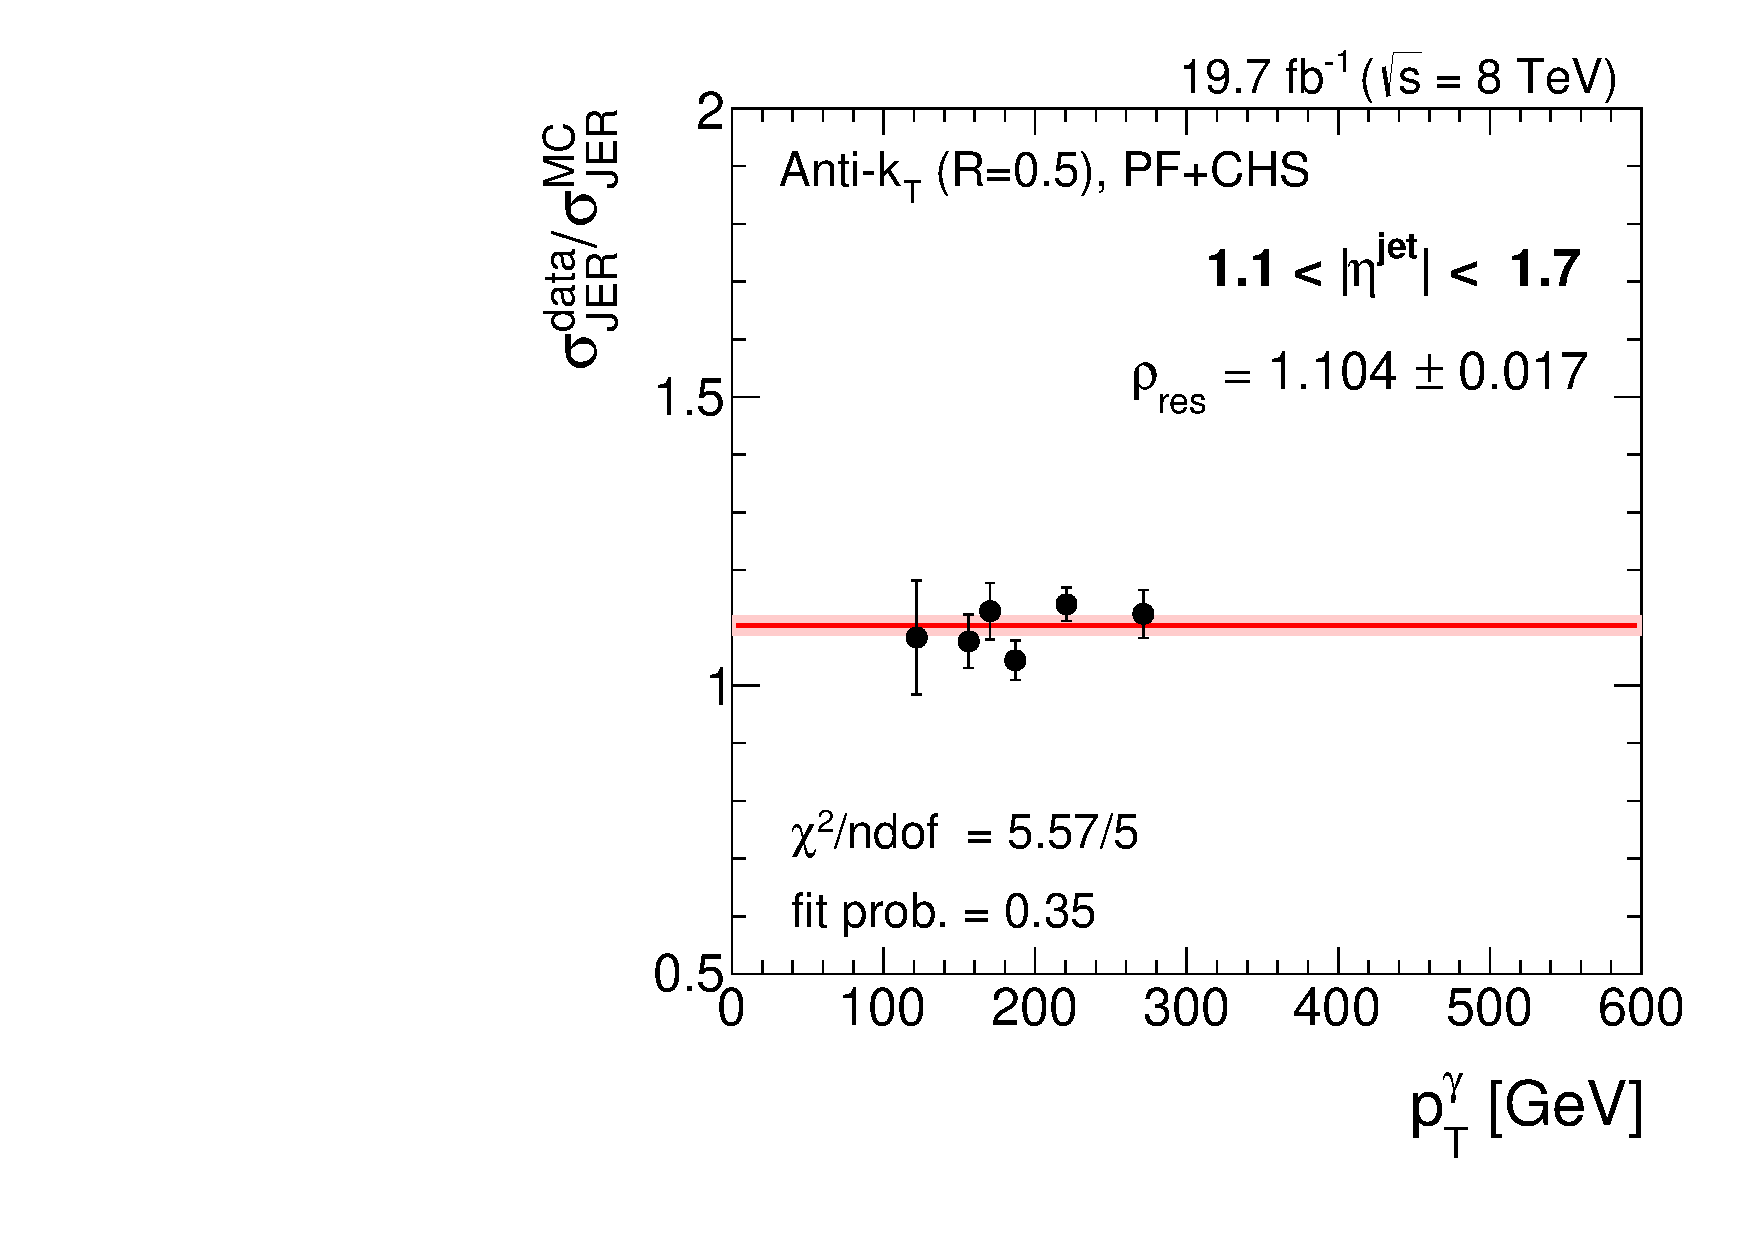
\includegraphics[width=0.49\textwidth]{figures/resolution/results/Ratio_Resolution_for_3_eta_bin_PFCHS_data_comparison_RMS99.pdf}
    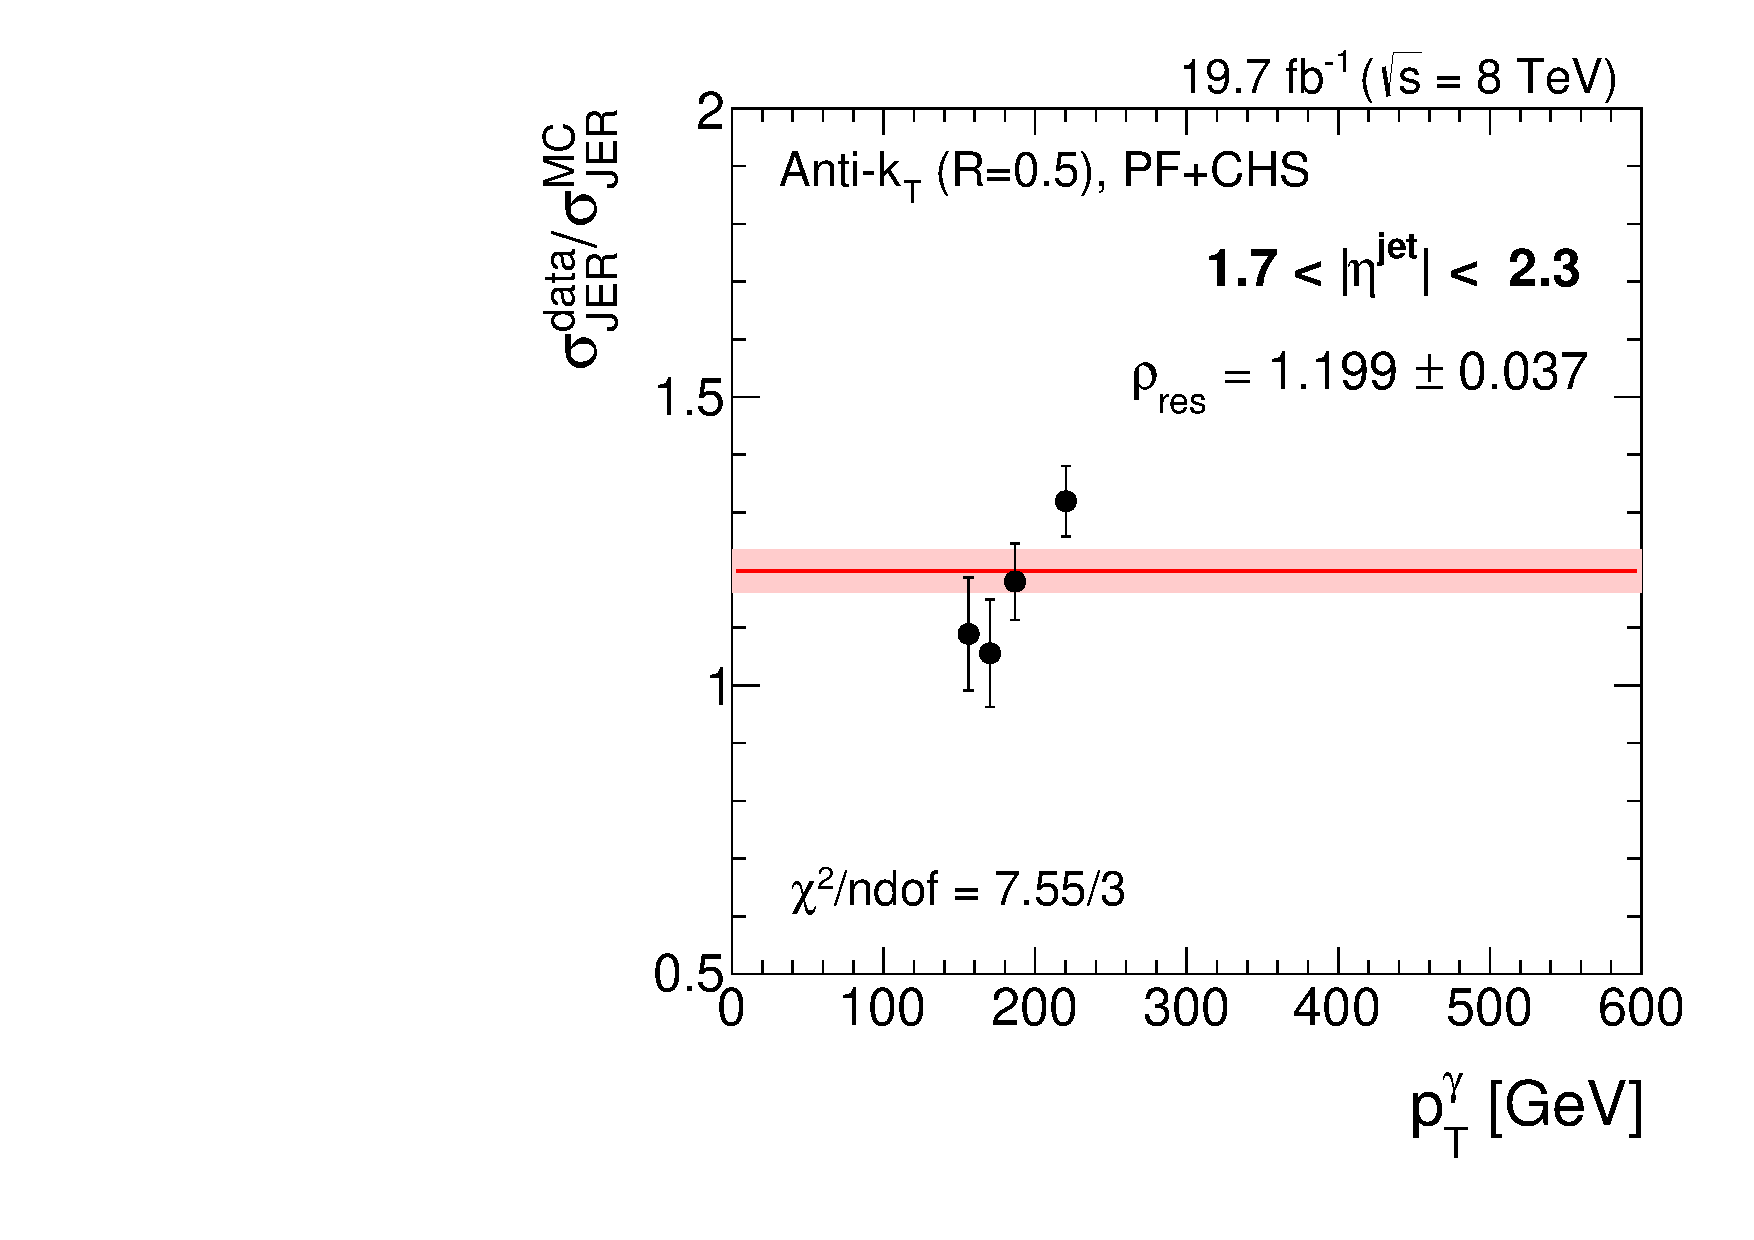
\includegraphics[width=0.49\textwidth]{figures/resolution/results/Ratio_Resolution_for_4_eta_bin_PFCHS_data_comparison_RMS99.pdf}
  \caption{Data to simulation resolution ratios, fitted with a horizontal line for four different $\eta^{\text{jet}}$-ranges: 
           \mbox{\subref{fig:Ratio1stEtaBin} $|\eta^{\text{1st jet}}| < 0.5$},
           \mbox{\subref{fig:Ratio2ndEtaBin} $0.5\le|\eta^{\text{1st jet}}| < 1.1$},
           \mbox{\subref{fig:Ratio3rdEtaBin} $1.1\le|\eta^{\text{1st jet}}| < 1.7$},
           \mbox{\subref{fig:Ratio4thEtaBin} $1.7\le|\eta^{\text{1st jet}}| < 2.3$}.}
  \label{fig:RatioEtaBinned}
\end{figure}

All fit results are greater then one which means that the resolution in data is in all bins worse compared to the resolution in simulation.
The values of the fits range from 1.067 (for the first $\eta$-bin) to 1.199 (for the last $\eta$-bin). 

The systematic uncertainties were evaluated as described in the previous chapter. 
The single uncertainties were taken as upper and lower boundary of the 68\% uncertainty band and were added in quadrature to get the total systematic uncertainty.
\mbox{Table \ref{tab:FinalResults}} summarizes the ratio results determined with data collected during the year 2012 with their statistical and systematic uncertainties.

\begin{table}[t]
\caption{Data to simulation resolution scaling factors with statistical and systematic uncertainties.}\renewcommand{\arraystretch}{2.0}
\large{
\begin{center}
\begin{tabular}{ | c | c   c c| }
$|\eta^{\text{Jet}}|$ & Ratio &  stat.      & sys.  \\\hline
$0.0 - 0.5$ &1.067 & $\pm 0.013$ & $^{+0.025}_{-0.024}$ \\
$0.5 - 1.1$ &1.087 & $\pm 0.013$ & $^{+0.039}_{-0.039}$ \\
$1.1 - 1.7$ &1.104 & $\pm 0.017$ & $^{+0.049}_{-0.049}$ \\
$1.7 - 2.3$ &1.199 & $\pm 0.037$ & $^{+0.075}_{-0.075}$ \\
\hline
\end{tabular}
\end{center}
}
\label{tab:FinalResults}
\end{table}

Though the $\GAMJET$ analysis is known to be capable to produce highly precise results, the systematic uncertainties are still dominating. 
The statistical limitation of this analysis is due to the collected data at the CMS detector. 
The number of simulated events is roughly eight times larger.
 
A comparison of the data to simulation resolution scaling factors between this analysis and the results of 2011 which were determined from a dijet data sample
\cite{Schroder:2012} can be found in \mbox{Fig. \ref{fig:RatioFinal}}.
The black dots show the $\frac{\text{JER}^{\text{data}}}{\text{JER}^{\text{MC}}}$ scale factors of the 2011 analysis with the gray band 
representing the statistical and systematic uncertainties added in quadrature while the magenta dots and the magenta band
are the 2012 central values with their total uncertainties.

\begin{figure}[b]
 \centering
    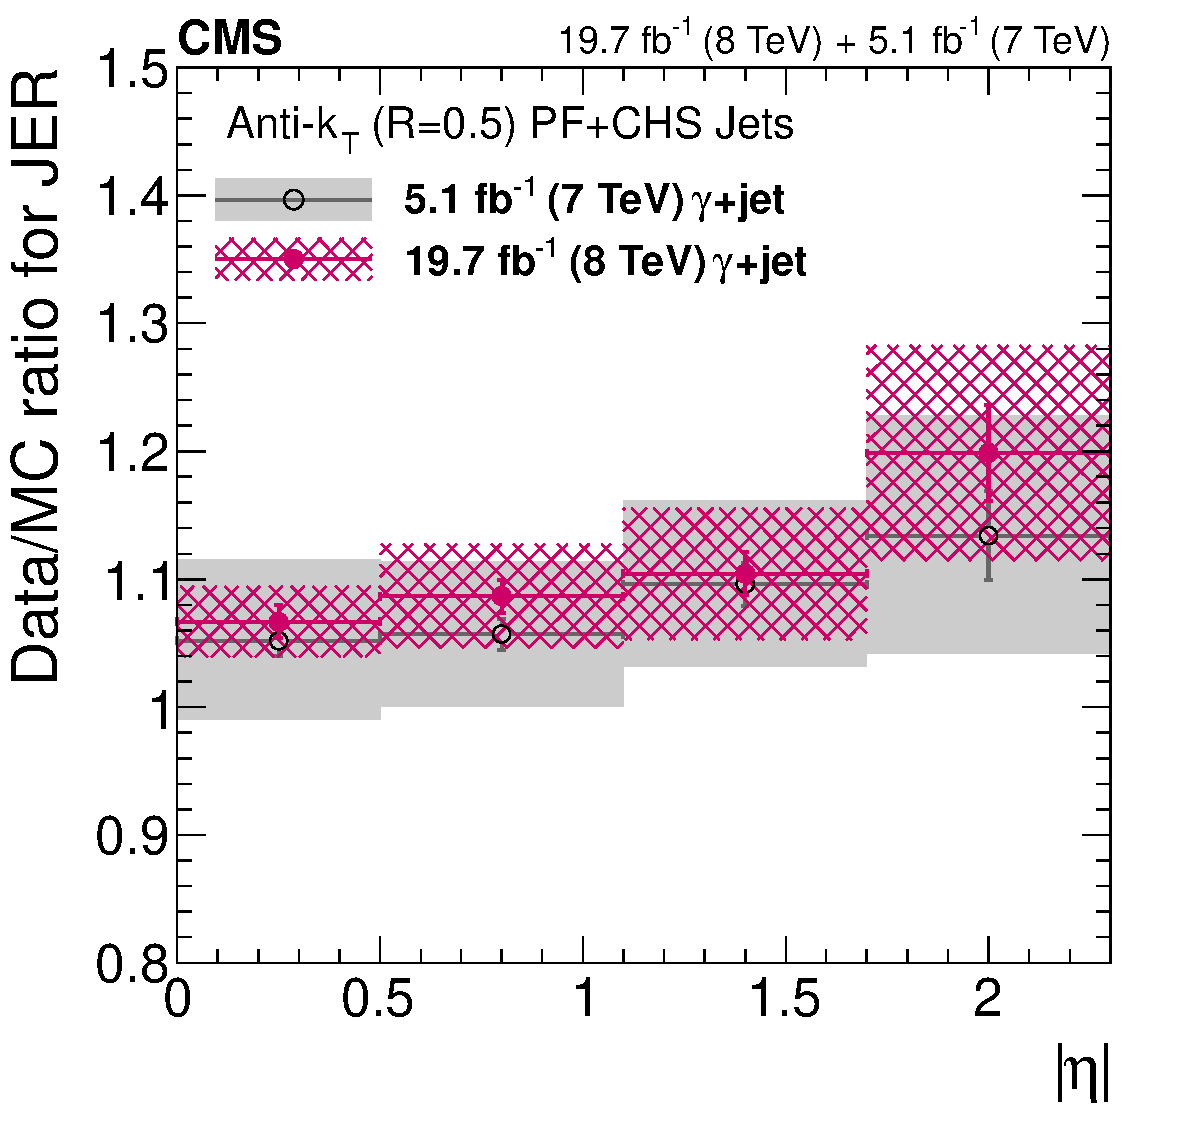
\includegraphics[width=0.6\textwidth]{figures/resolution/results/resultsComparisonFINAL.pdf}
  \caption{The measured data to simulation resolution ratio $\frac{\text{JER}^{\text{data}}}{\text{JER}^{\text{MC}}}$ for 2012 (magenta dots) and 2011 (black dots)
           with statistical and systematic uncertainties added in quadrature (magenta area). The dark gray line indicates the systematic uncertainty only.}
  \label{fig:RatioFinal}
\end{figure}

It can be seen, that throughout the whole $\eta^{\text{jet}}$-range the data to simulation scale factors became systematically larger. 


Comparing the precision of both measurements, the $\GAMJET$ analysis is for all $\eta$-bins more precise than the analysis done with dijet events.
This is due to the smaller systematic uncertainties of the $\GAMJET$ analysis which compensates for the better statistical precision of the dijet sample due to the large 
cross section.



%%%%%%%%%%%%%%%%%%%%%%%%%%%%%%%%%%%%%%%%%%%%%%%%%%%%%%%%%%%%%%%%%%%%%%%%%%%%%%%%%%%%%%%%%%%%%%%%%%%%%%%%%%%%%%%%%%%%%%%%%%%%%%%%%%%%%%%%%%%%%%%%%%%%%%%%%%%%%%%%%%%%%%%%%%%%%%%%%%%%%%%%%%%%%%%%%%%%%%%%%%%%%%%%%%%%%%%%%%%%%%%%%%%%%%%%%%%

%%%%%%%%%%%%%%%%%%%%%%%%%%%%%%%%%%%%%%%%%%%%%%%%%%%%%%%%%%%%%%%%%%%%%%%%%%%%%%%%%%%%%%%%%%%%%%%%%%%%%%%%%%%%%%%%%%%%%%%%%%%%%%%%%%%%%%%%%%%%%%%%%%%%%%%%%%%%%%%%%%%%%%%%%%%%%%%%%%%%%%%%%%%%%%%%%%%%%%%%%%%%%%%%%%%%%%%%%%%%%%%%%%%%%%%%%%%
%%%%%%%%%%%%%%%%%%%%%%%%%%%%%%%%%%%%%%%%%%%%%%%%%%%%%%%%%%%%%%%%%%%%%%%%%%%%%%%%%%%%%%%%%%%%%%%%%%%%%%%%%%%%%%%%%%%%%%%%%%%%%%%%%%%%%%%%%%%%%%%%%%%%%%%%%%%%%%%%%%%%%%%%%%%%%%%%%%%%%%%%%%%%%%%%%%%%%%%%%%%%%%%%%%%%%%%%%%%%%%%%%%%%%%%%%%%
\FloatBarrier
\chapter{Discussion and conclusion}
A first measurement of the resolution ratio $\frac{\text{JER}^{\text{data}}}{\text{JER}^{\text{MC}}}$ 
using $\GAMJET$ events with $19.7\fbinv$ pp collision data at $\sqrt{s}=8 \tev$ collected in 2012 at the CMS detector has been presented. 
For this purpose, the methodology introduced in \cite{CMS-AN-2010-076}
was further developed to take account of the double peak structure when applying an exclusive binning in the variable $\alpha$ 
that measures the additional jet activity in the event.

The resolution in data was found to be systematically larger than in the simulation throughout the investigated $\eta^{\text{jet}}$ plane. 
A possible $\pt^{\gamma}$ dependence of the resolution scale factors was not visible. 
Thus, the ratio has been parametrized with a constant per $\eta^{\text{jet}}$ bin.

The relative difference of the data resolution ranges from $\sim$ 7\% to $\sim$ 20\% for  $0.0<|\eta^{\text{jet}}|<0.5$ and  $1.7<|\eta^{\text{jet}}|<2.3$, respectively, 
with total statistical and systematic uncertainties between 3\% and 8\%.



\begin{itemize}
\item Repeat results
\item cross-check analysis
\item Outlook
\end{itemize}

